The event selection aims at rejecting events that do not match the decay signatures targeted by this analysis. We require that at least two leptons passing the tight selection are present in the event. Moreover, events where a pair of loose leptons with an invariant mass smaller than 12\GeV is found are rejected, as they are not modeled by the simulation.

For all events passing the selection, we require at least two jets with transverse momentum greater than 25\GeV be reconstructed in the $|\eta|<2.4$ region.
We also require that both jets satisfy the loose working point of the CSV $\cPqb$-tag algorithm, or that at least one of them satisfies the medium working point,
as a top quark pair decaying into $\cPqb$-jets is present in all signal events.

\subsection{Two lepton same-sign category}

In events where no additional tight lepton with a transverse momentum greater than 10\GeV is present, we require that the two tight leptons have the same charge and transverse momenta greater than 25\GeV and 15\GeV respectively. These events constitute the two lepton same-sign (\textit{2lss}) category of the analysis. % If the sub-leading lepton is an electron, and only for this category, its transverse momentum requirement is tightened to 15\GeV.

In addition to the requirements described above, we discard 2lss events that contain less than four jets with transverse momentum greater than 25\GeV and $|\eta|<2.4$ in the final state.

The event is also rejected if the two selected leptons do not pass the requirements aimed at rejecting leptons from conversions and those on the quality of the charge measurement described in Section~\ref{sec:objects}.
The background from electrons from $\Z$ decays, where the charge of one electron is mismeasured, is further reduced by vetoing events where the di-electron invariant mass differs by less than 10\GeV from the $\Z$ mass. For the same reason, we also require that the $E_\mathrm{T}^\mathrm{miss}LD$ variable is larger than 0.2 in di-electron events. 

\subsection{Three and four lepton categories}
The three lepton (\textit{3l}) category consists of events that contain exactly three tight leptons with a transverse momenta greater than 25, 15 and 15 \GeV respectively. 
%No requirement is applied on the possible presence of an even larger number of leptons; i.e., this category implicitly includes events with four or more leptons.
In order to reject backgrounds from processes with $\Z$ bosons in the final state, we require that no pair of same-flavor opposite-sign loose leptons has an invariant mass closer than 10\GeV to the mass of the $\Z$ boson. We then add an $E_\mathrm{T}^\mathrm{miss}LD > 0.2$ requirement.
The $E_\mathrm{T}^\mathrm{miss}LD$ threshold is tighter (0.3)
if the event has a pair of leptons with the same flavor and opposite sign. 
For events with large jet multiplicity ($\geq$ 4 jets), where the contamination
from the $\Z$ background is smaller, no requirement
on $E_\mathrm{T}^\mathrm{miss}LD$ is applied.
The event is also rejected if the three selected leptons do not pass the conversion veto requirements, or if the sum of their charges is not equal to +1 or -1.
We further veto events with two OSSF pairs and their 4 lepton mass lower than 140 GeV, where the leptons pass the loose identification.

The four lepton (\textit{4l}) category is defined exactly as the (\textit{3l}) category, except that it requires the presence of 
at least four tight leptons with a transverse momenta greater than 25, 15, 15, and 10 \GeV respectively.

%The observed event yields in data for each final state and the
%expectations from the different physical processes are summarised in
%table~\ref{tab:yields-sel}.

%\begin{table}[thb]
%\centering
%\begin{tabular}{l@{\qquad}rrr@{\qquad}r}\hline
%\multicolumn{1}{c@{\qquad}}{} &
%\multicolumn{1}{c}{$\Pgm\Pgm$} &
%\multicolumn{1}{c}{$\Pe\Pe$} &
%\multicolumn{1}{c@{\qquad}}{$\Pe\Pgm$} &
%\multicolumn{1}{c@{\qquad}}{$3\ell$} \\ \hline
%
%$\ttbar\,\PW$                 & $ 18.2 \pm 0.9   $&$  6.9 \pm 0.6       $&$ 24.6  \pm 1.1    $&$ 12.3   \pm 0.7   $ \\
%$\ttbar\,\Z\!/\!\gamma^*$     & $  5.8 \pm 0.6   $&$  7.5 \pm 0.6       $&$ 15.3  \pm 1.3    $&$ 22.7   \pm 1.0   $ \\ \hline
%di-boson                      & $  1.4 \pm 0.2   $&$  1.1 \pm 0.2       $&$  2.6 \pm  0.3    $&$ 5.7   \pm  0.4   $ \\
%$\mathrm{tttt}$               & $  0.8 \pm 0.2   $&$  0.4 \pm 0.1       $&$  1.5 \pm  0.2    $&$ 1.2   \pm  0.1   $ \\
%$\mathrm{tqZ}$                & $  0.2 \pm 0.3   $&$  0.4 \pm 0.4       $&$  0.6 \pm  0.6    $&$ 2.7   \pm  0.8   $ \\
%rare backgrounds              & $  1.6 \pm 0.3   $&$  0.5 \pm 0.1       $&$  1.8 \pm  0.1    $&$ 0.3   \pm  0.1   $ \\ \hline \hline      
%non-prompt (MC)               & $ 24.0 \pm 1.3   $&$  11.1 \pm 1.0      $&$  41.5 \pm 2.0    $&$ 28.3  \pm  1.5   $ \\ 
%charge mis-ID (MC)            &                   &$  5.8 \pm 2.3       $&$  6.6  \pm 1.7    $&$                  $ \\  \hline
%non-prompt (data-driven)      & $ 33.4 \pm 1.2   $&$ 23.1 \pm 1.1       $&$  61.9 \pm 1.7    $&$ 51.0   \pm 1.8   $ \\
%charge mis-ID (data-driven)   &                   &$  6.7 \pm 0.1       $&$  10.0 \pm 0.1    $&                     \\ \hline \hline
%all backgrounds (MC)          & $ 52.0 \pm 1.8   $&$  33.8 \pm 2.7      $&$  94.6 \pm 3.2    $&$ 73.2  \pm 2.1    $ \\
%all backgrounds (data-driven) & $ 61.3 \pm 1.7   $&$  46.6 \pm 1.5      $&$  118.2 \pm 2.5   $&$ 95.9   \pm 2.3   $ \\ \hline \hline
%$\ttH$                        & $  8.0 \pm 0.2   $&$  3.4 \pm 0.1       $&$  11.3 \pm 0.2    $&$ 10.8   \pm 0.2   $ \\ \hline \hline
%data                          &    74                    &   45                      &    154         &    105      \\ \hline
%\end{tabular}
%\caption{Expected and observed yields after the selection in all final states. The rare SM backgrounds include triboson, $\PW^\pm\PW^\pm\mathrm{qq}$, and $\PW\PW$ produced in double-parton interactions. Uncertainties are statistical only.}
%\label{tab:yields-sel}
%\end{table}

Figures~\ref{fig:2l_lepPt}-\ref{fig:2l_metLD} and \ref{fig:3l_lepPt}-\ref{fig:3l_ht} show the main event observables (lepton and jet multiplicities and spectra, energy sums) for events passing the $2\ell$ and $3\ell$. Figure \ref{fig:4l_numevt} shows the number of events in the $4\ell$ category.

%%%%%
%%   2l plots
%%%%%

%\begin{figure}[htb]
%	\centering 
%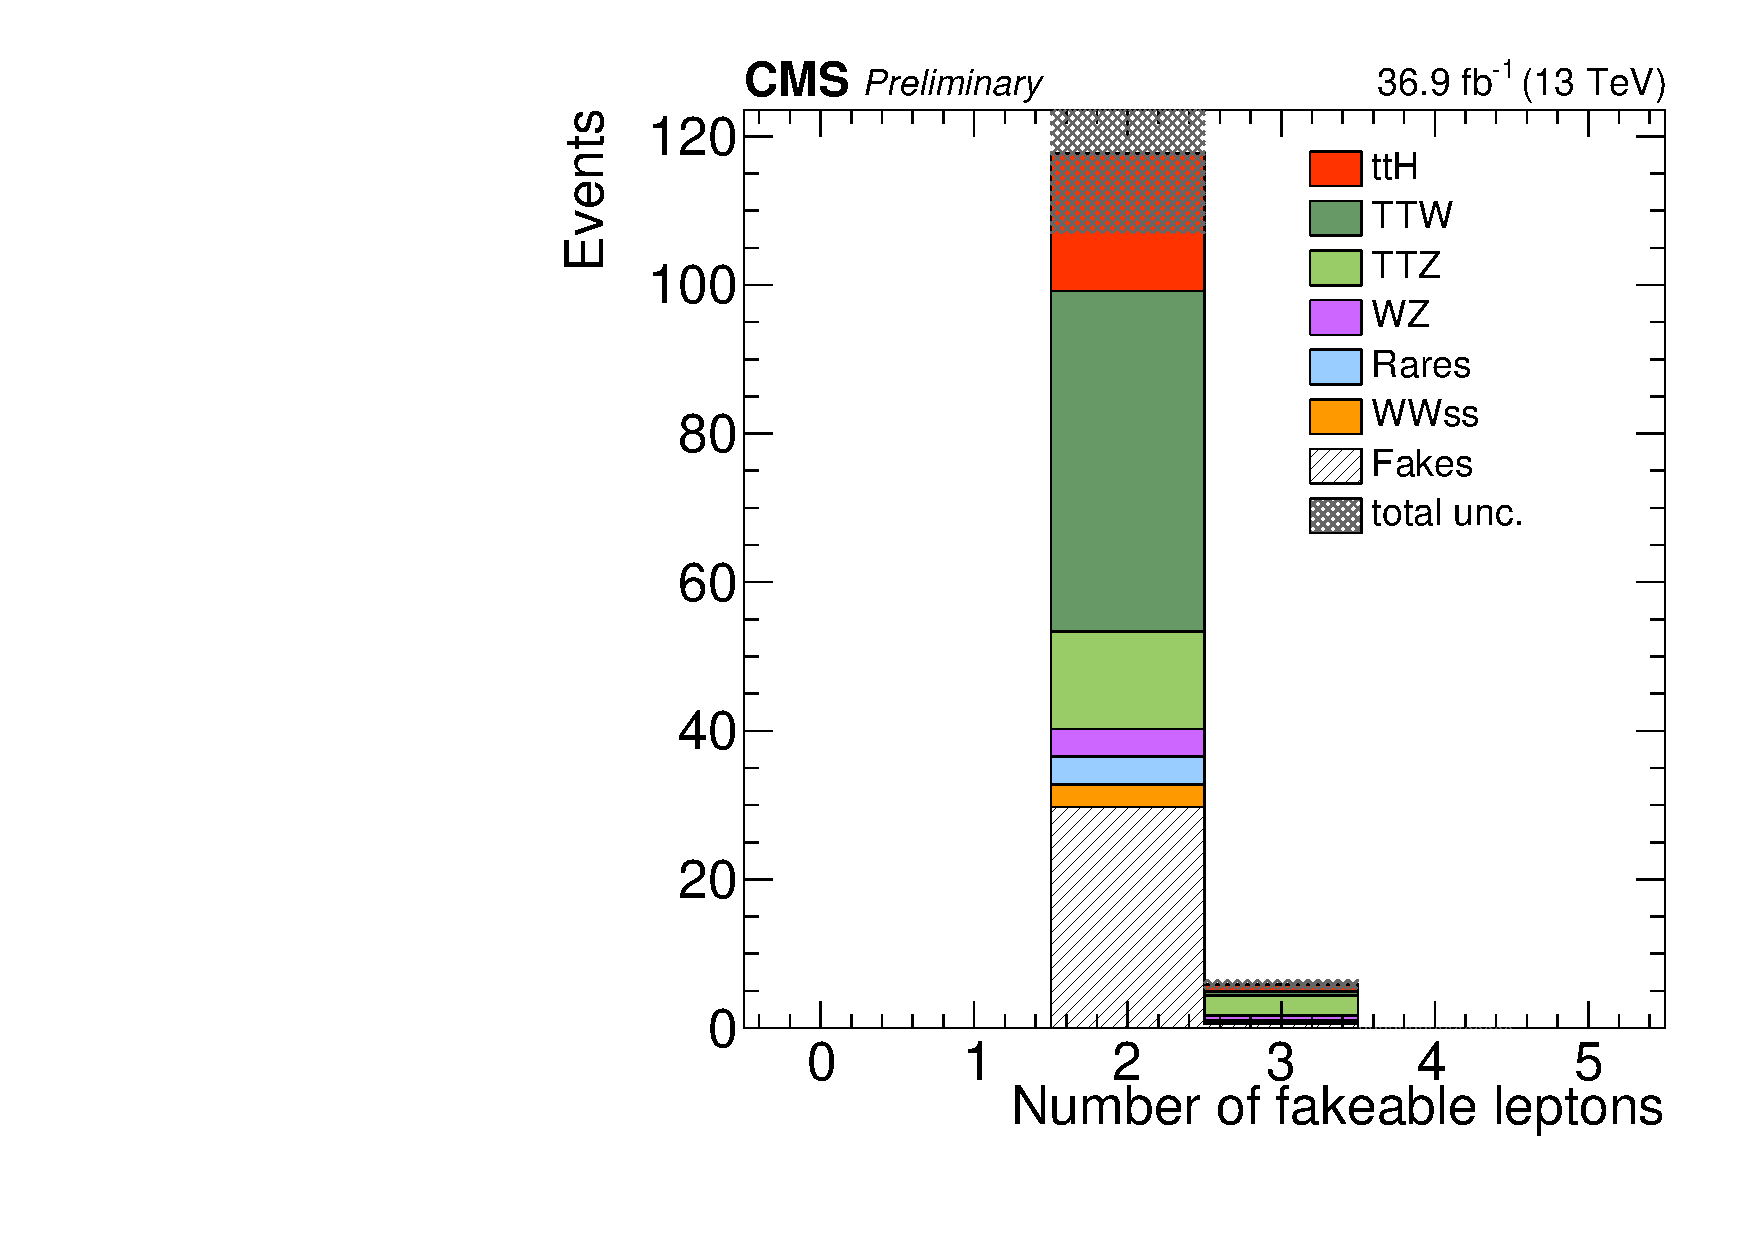
\includegraphics[width=0.32\textwidth]{plots_leptons/lep_evtsel/2lss_SR/mm/nLepFO.pdf}
%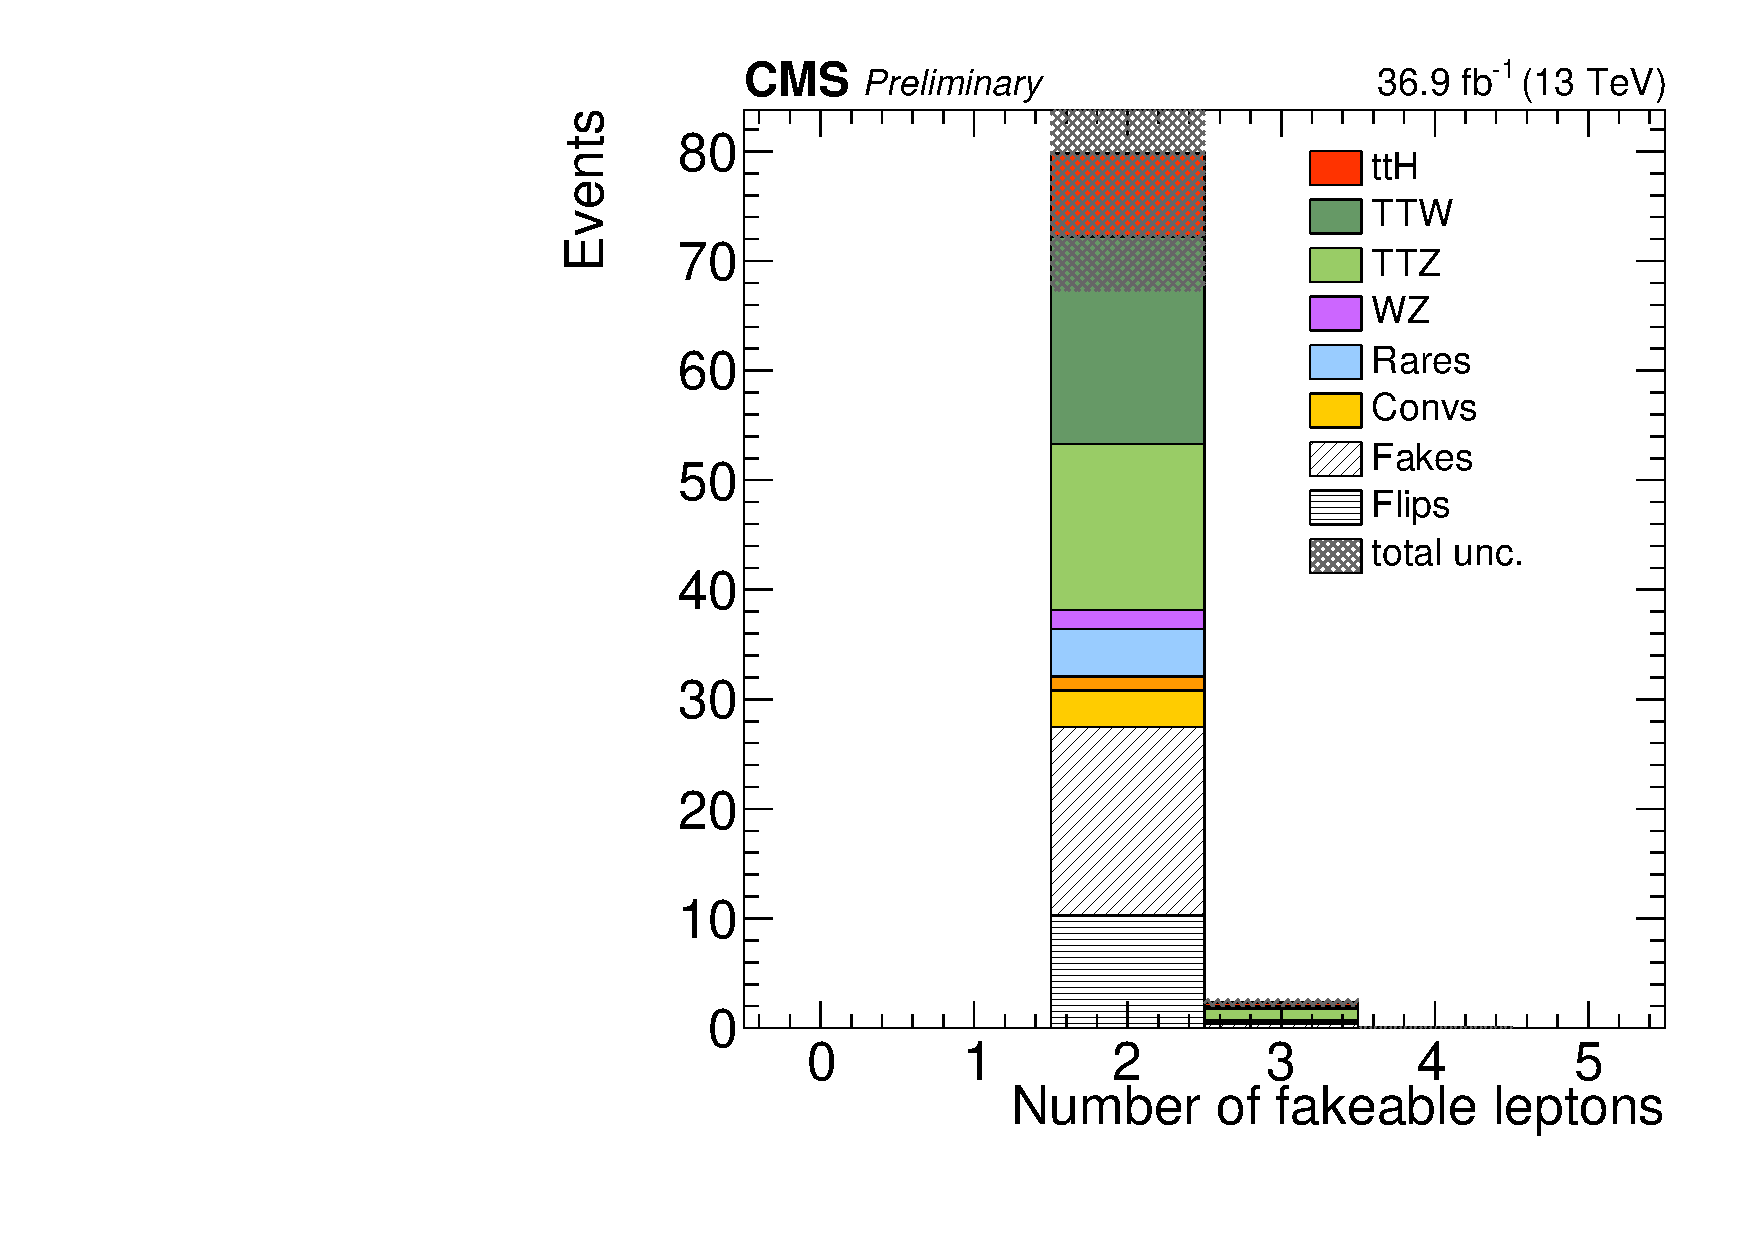
\includegraphics[width=0.32\textwidth]{plots_leptons/lep_evtsel/2lss_SR/ee/nLepFO.pdf}
%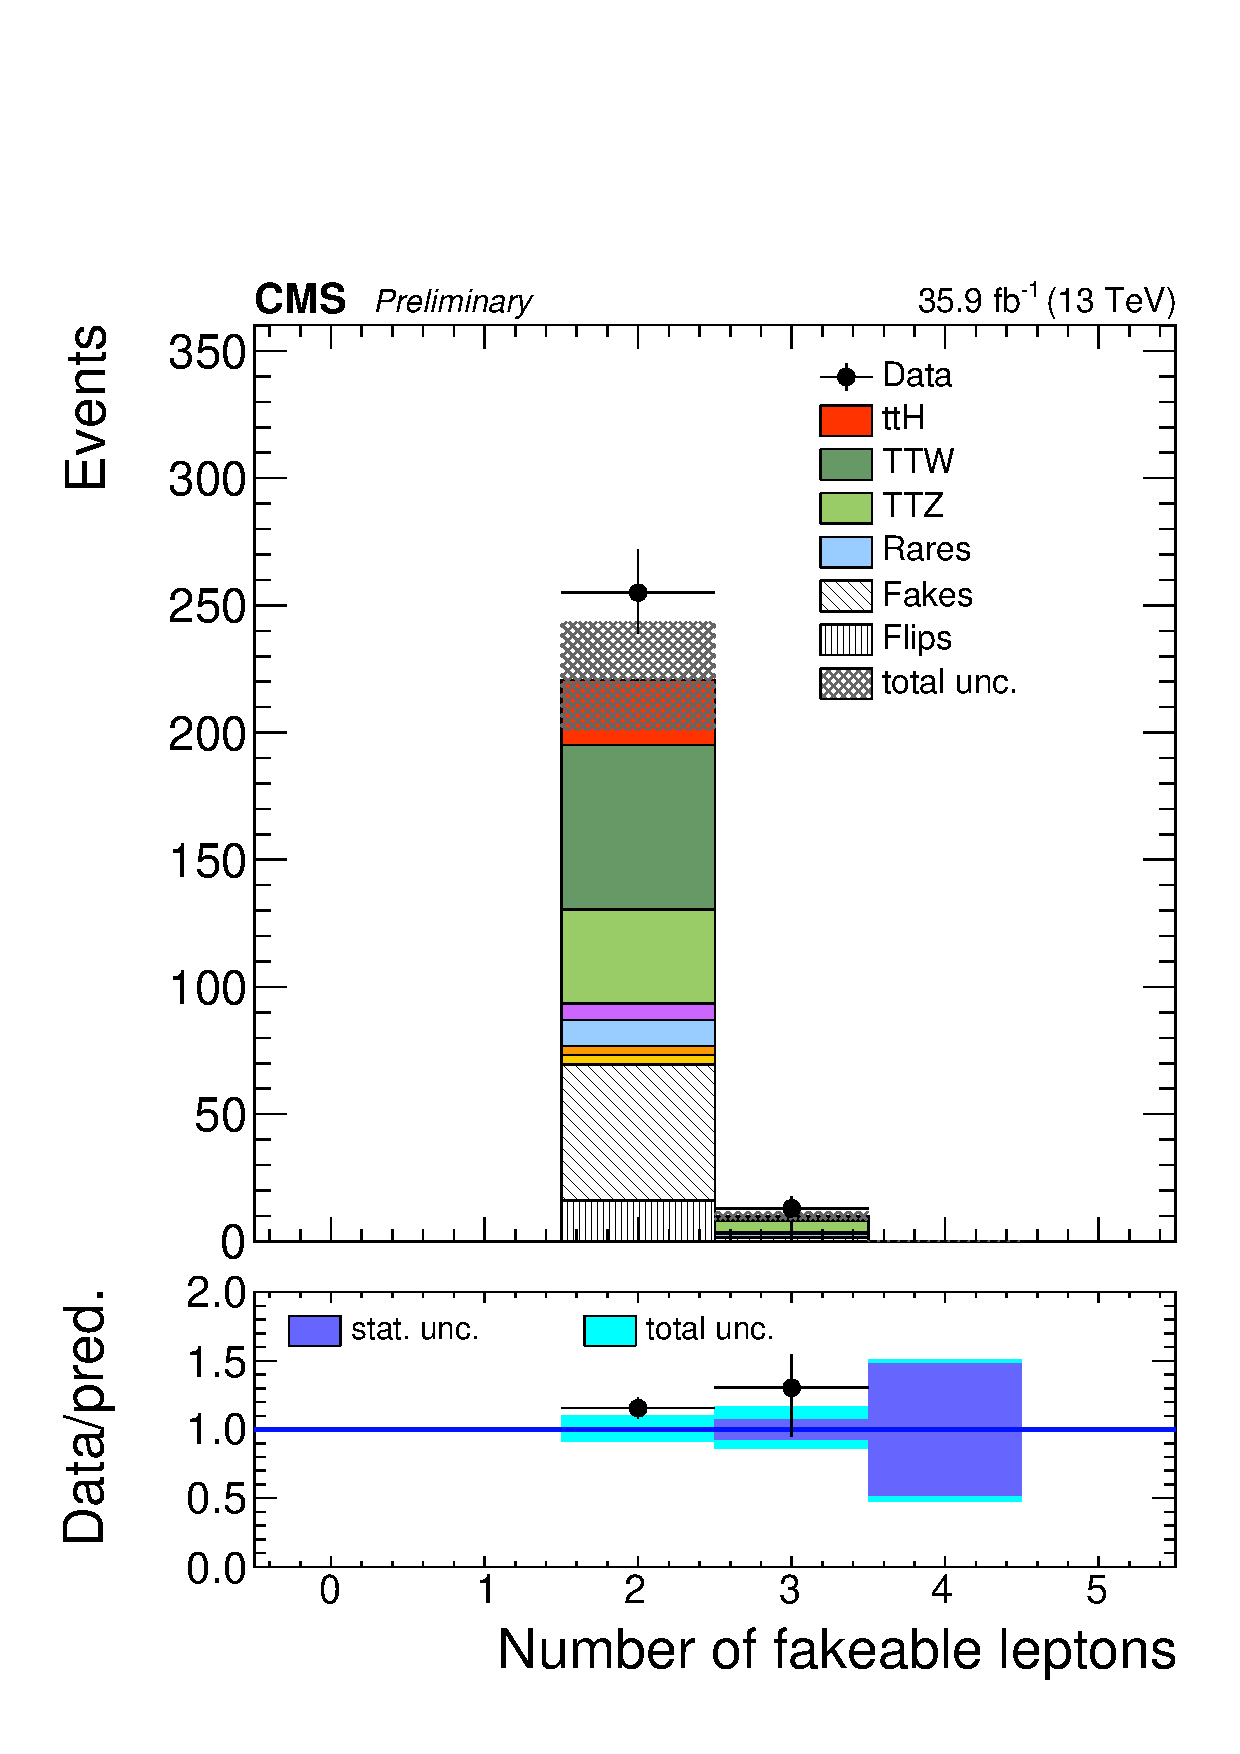
\includegraphics[width=0.32\textwidth]{plots_leptons/lep_evtsel/2lss_SR/em/nLepFO.pdf}
%	\caption{Number of leptons passing the fakeable object requirements in the 2$\ell$ ($\Pgm\Pgm$, $\Pe\Pe$, $\Pe\Pgm$) selections.}
%	\label{fig:2l_nLepFO}
%\end{figure}

%\begin{figure}[htb]
%	\centering 
%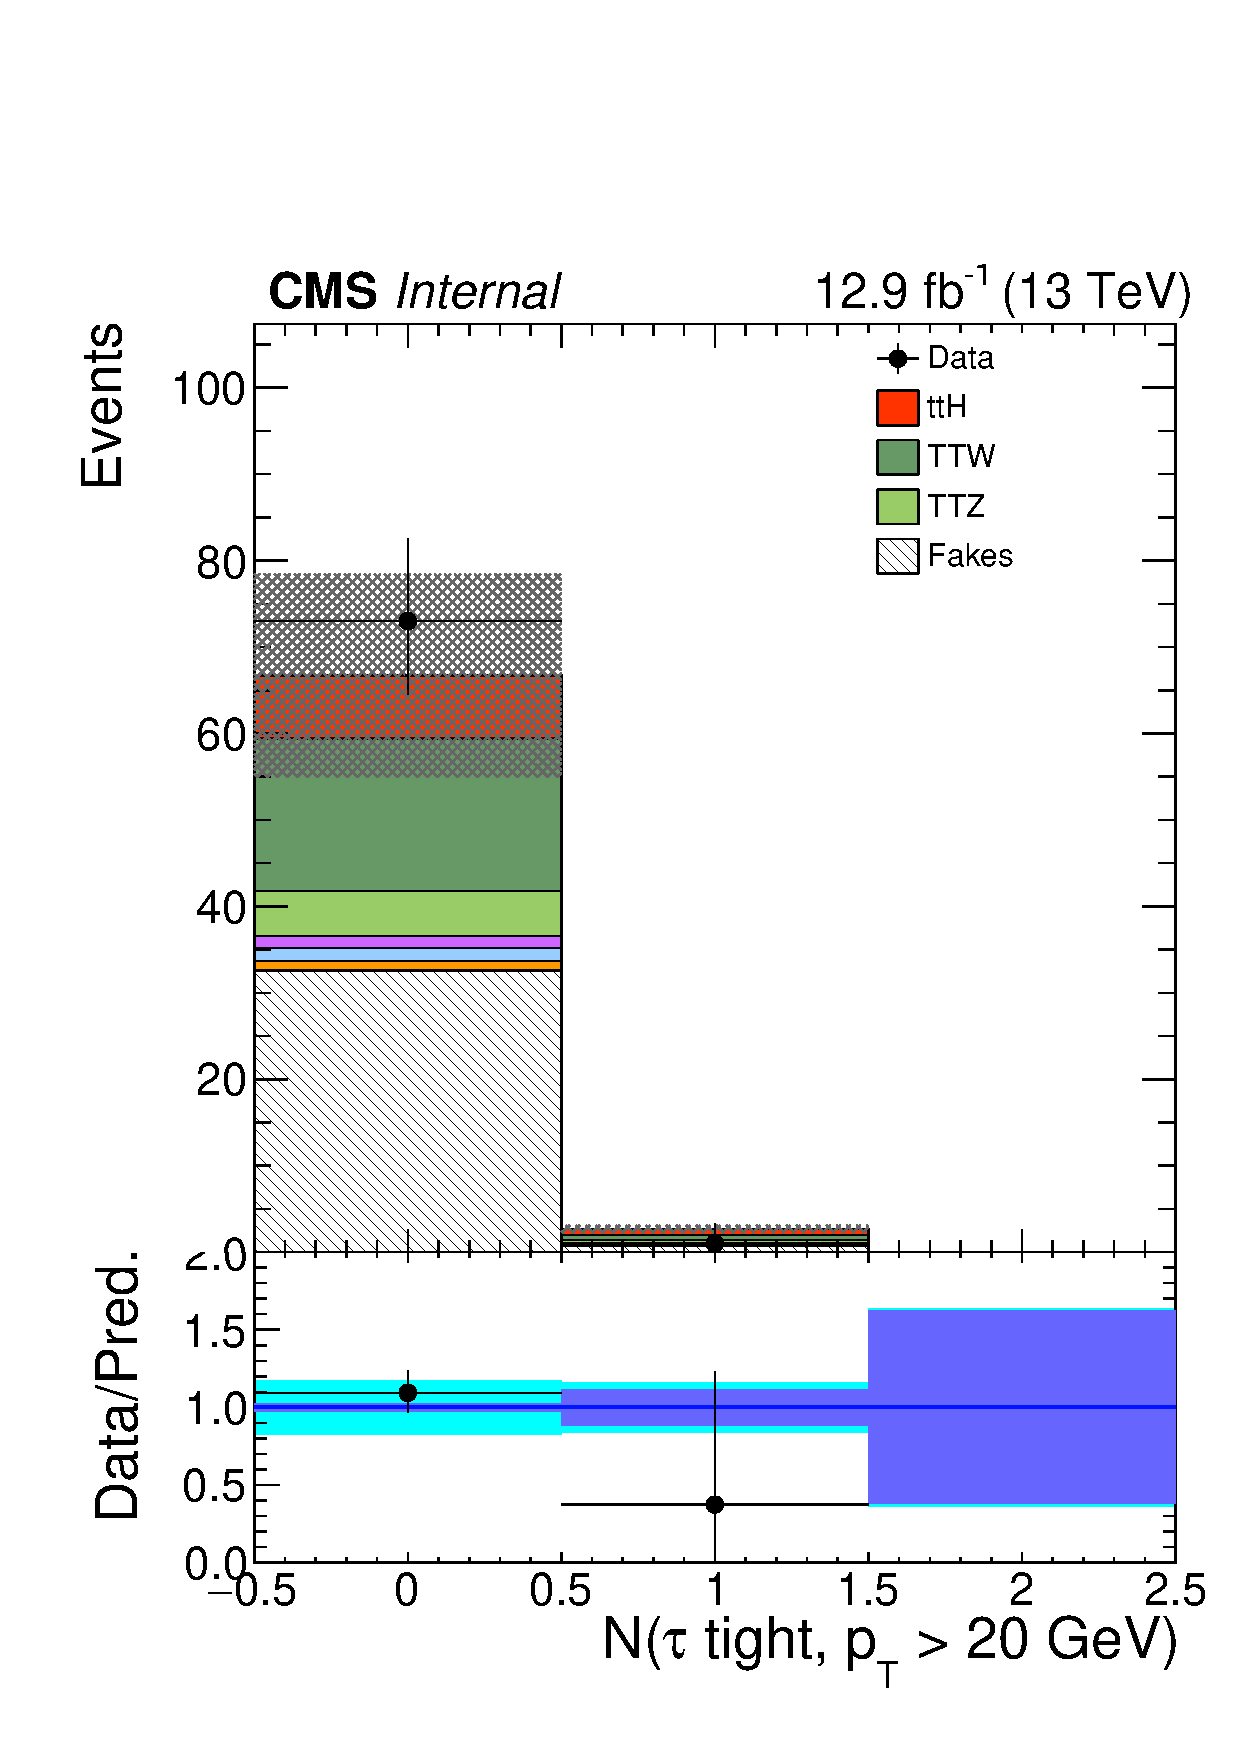
\includegraphics[width=0.32\textwidth]{plots_leptons/lep_evtsel/2lss_SR/mm/nTauTight}
%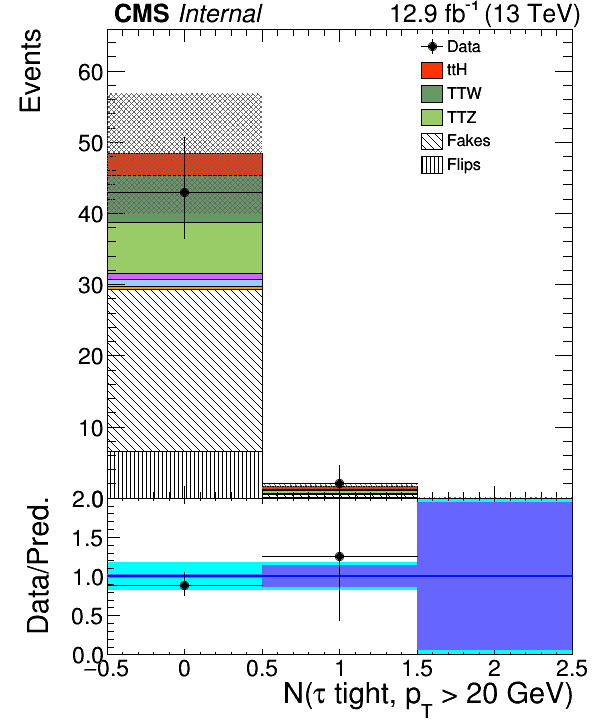
\includegraphics[width=0.32\textwidth]{plots_leptons/lep_evtsel/2lss_SR/ee/nTauTight}
%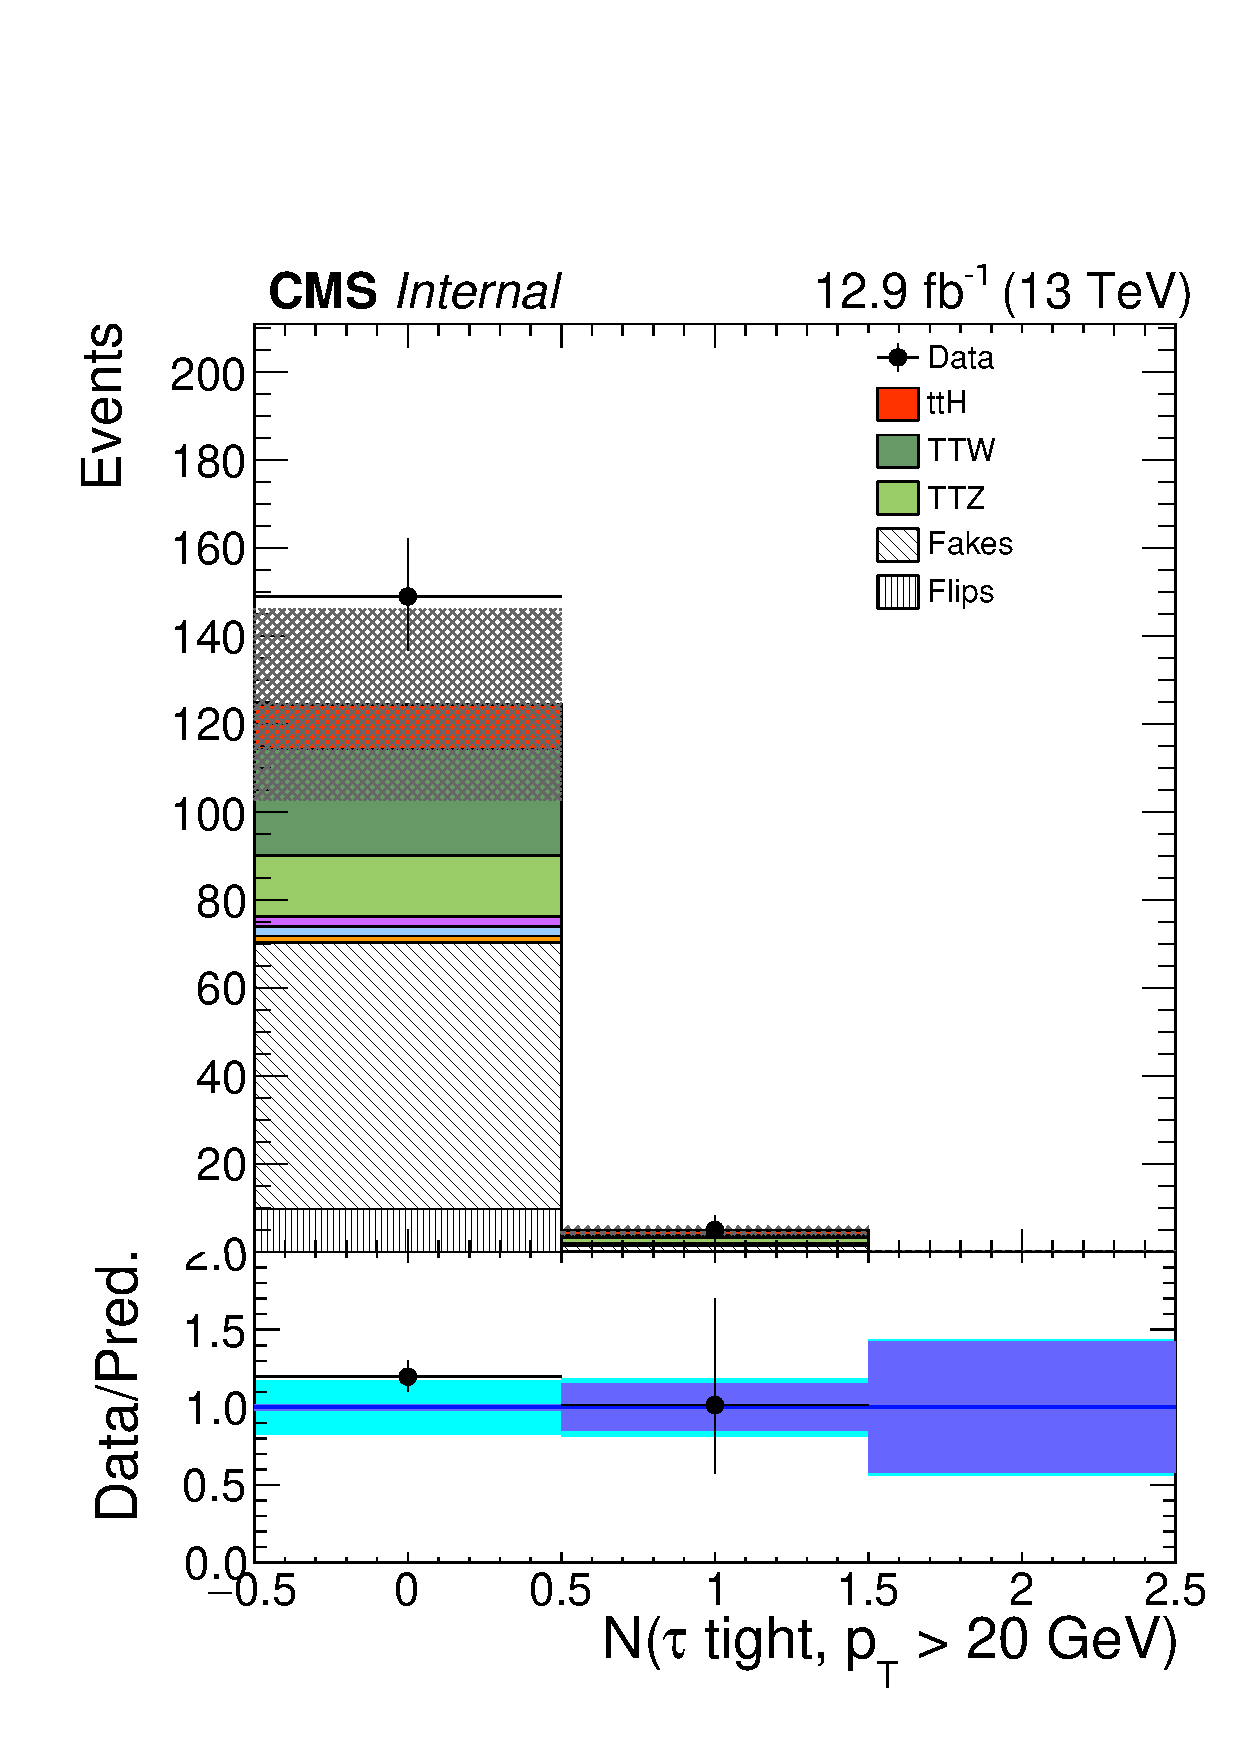
\includegraphics[width=0.32\textwidth]{plots_leptons/lep_evtsel/2lss_SR/em/nTauTight}
%	\caption{Number of reconstructed $\Pgth$ leptons passing the requirements described in Section~\ref{subsec:taus} in the 2$\ell$ ($\Pgm\Pgm$, $\Pe\Pe$, $\Pe\Pgm$) selections.}
%	\label{fig:2l_nTau}
%\end{figure}

\begin{figure}[htb]
	\centering 
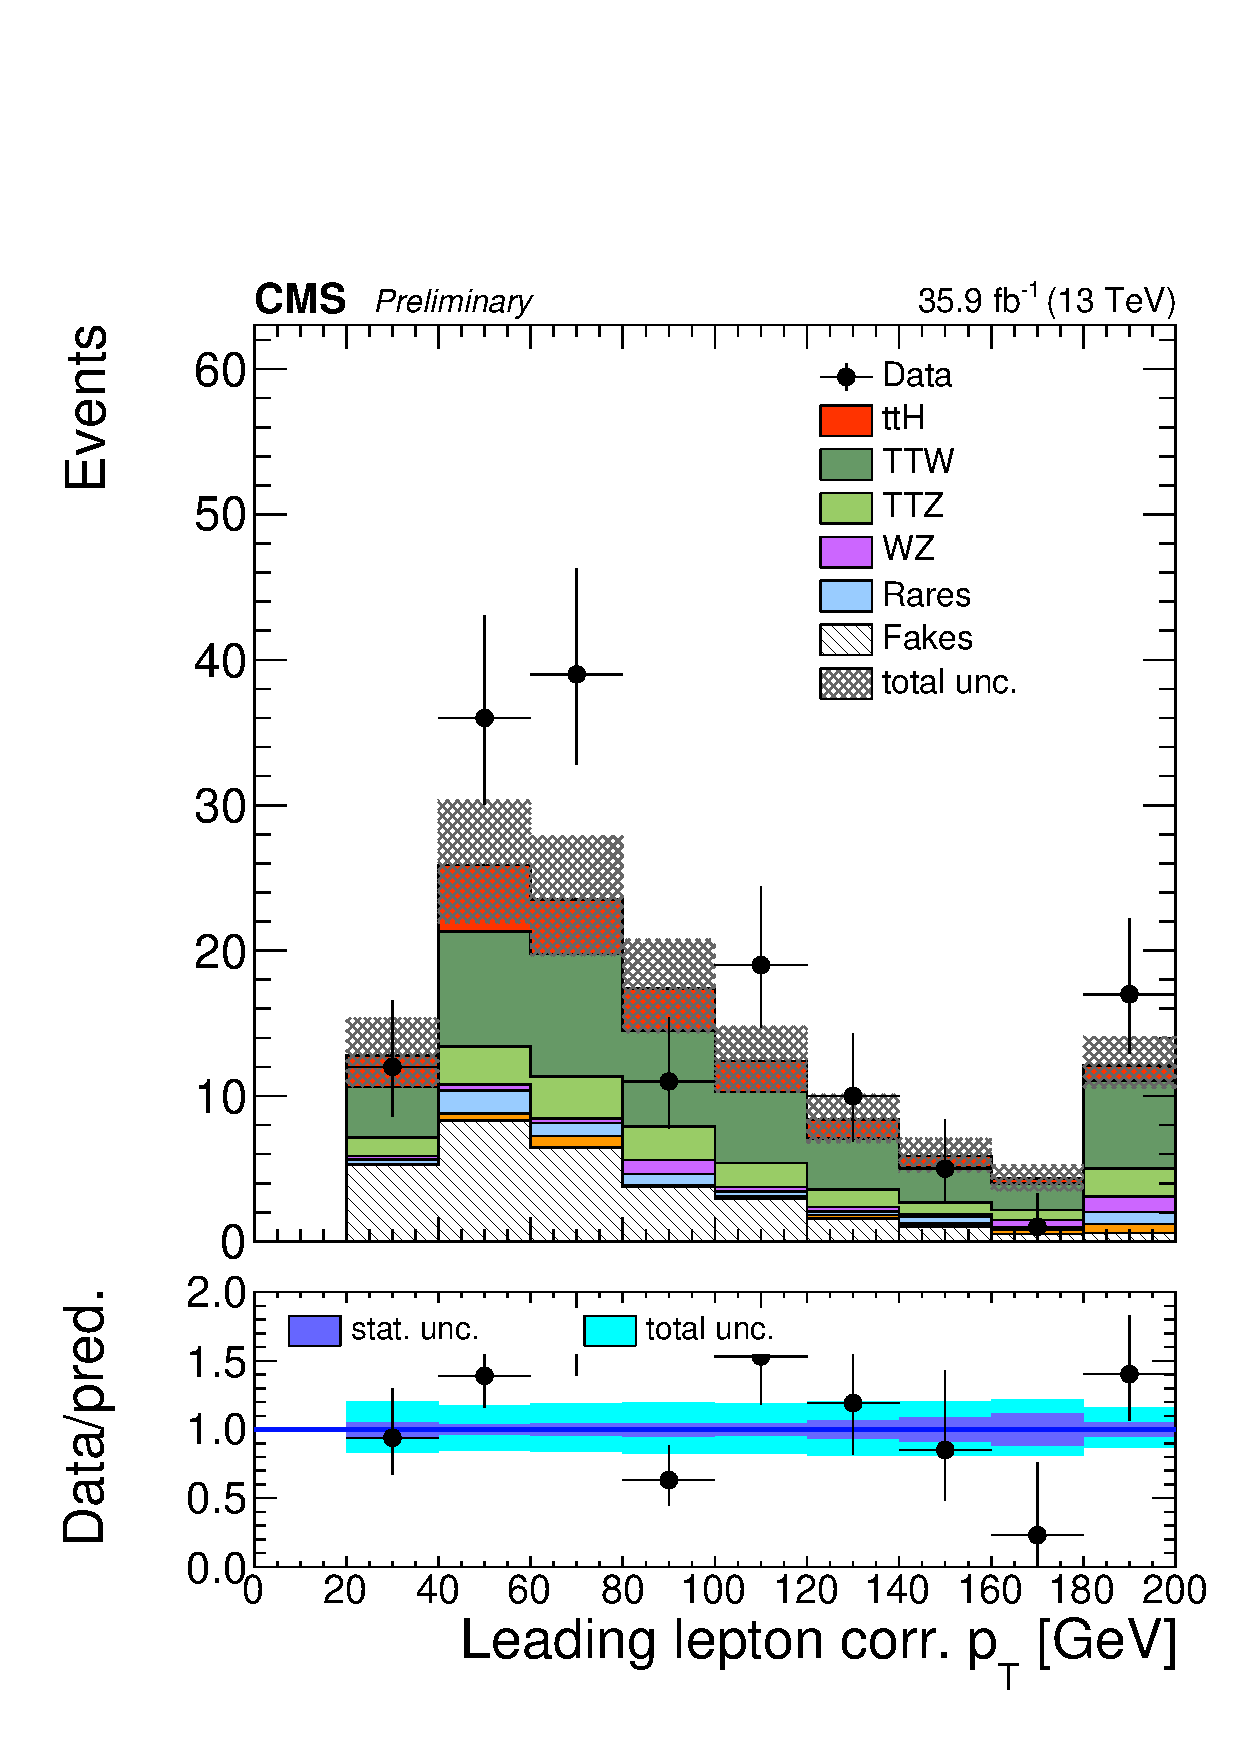
\includegraphics[width=0.32\textwidth]{plots_leptons/lep_evtsel/2lss_SR/mm/kinMVA_input_LepGood0_conePt.pdf}
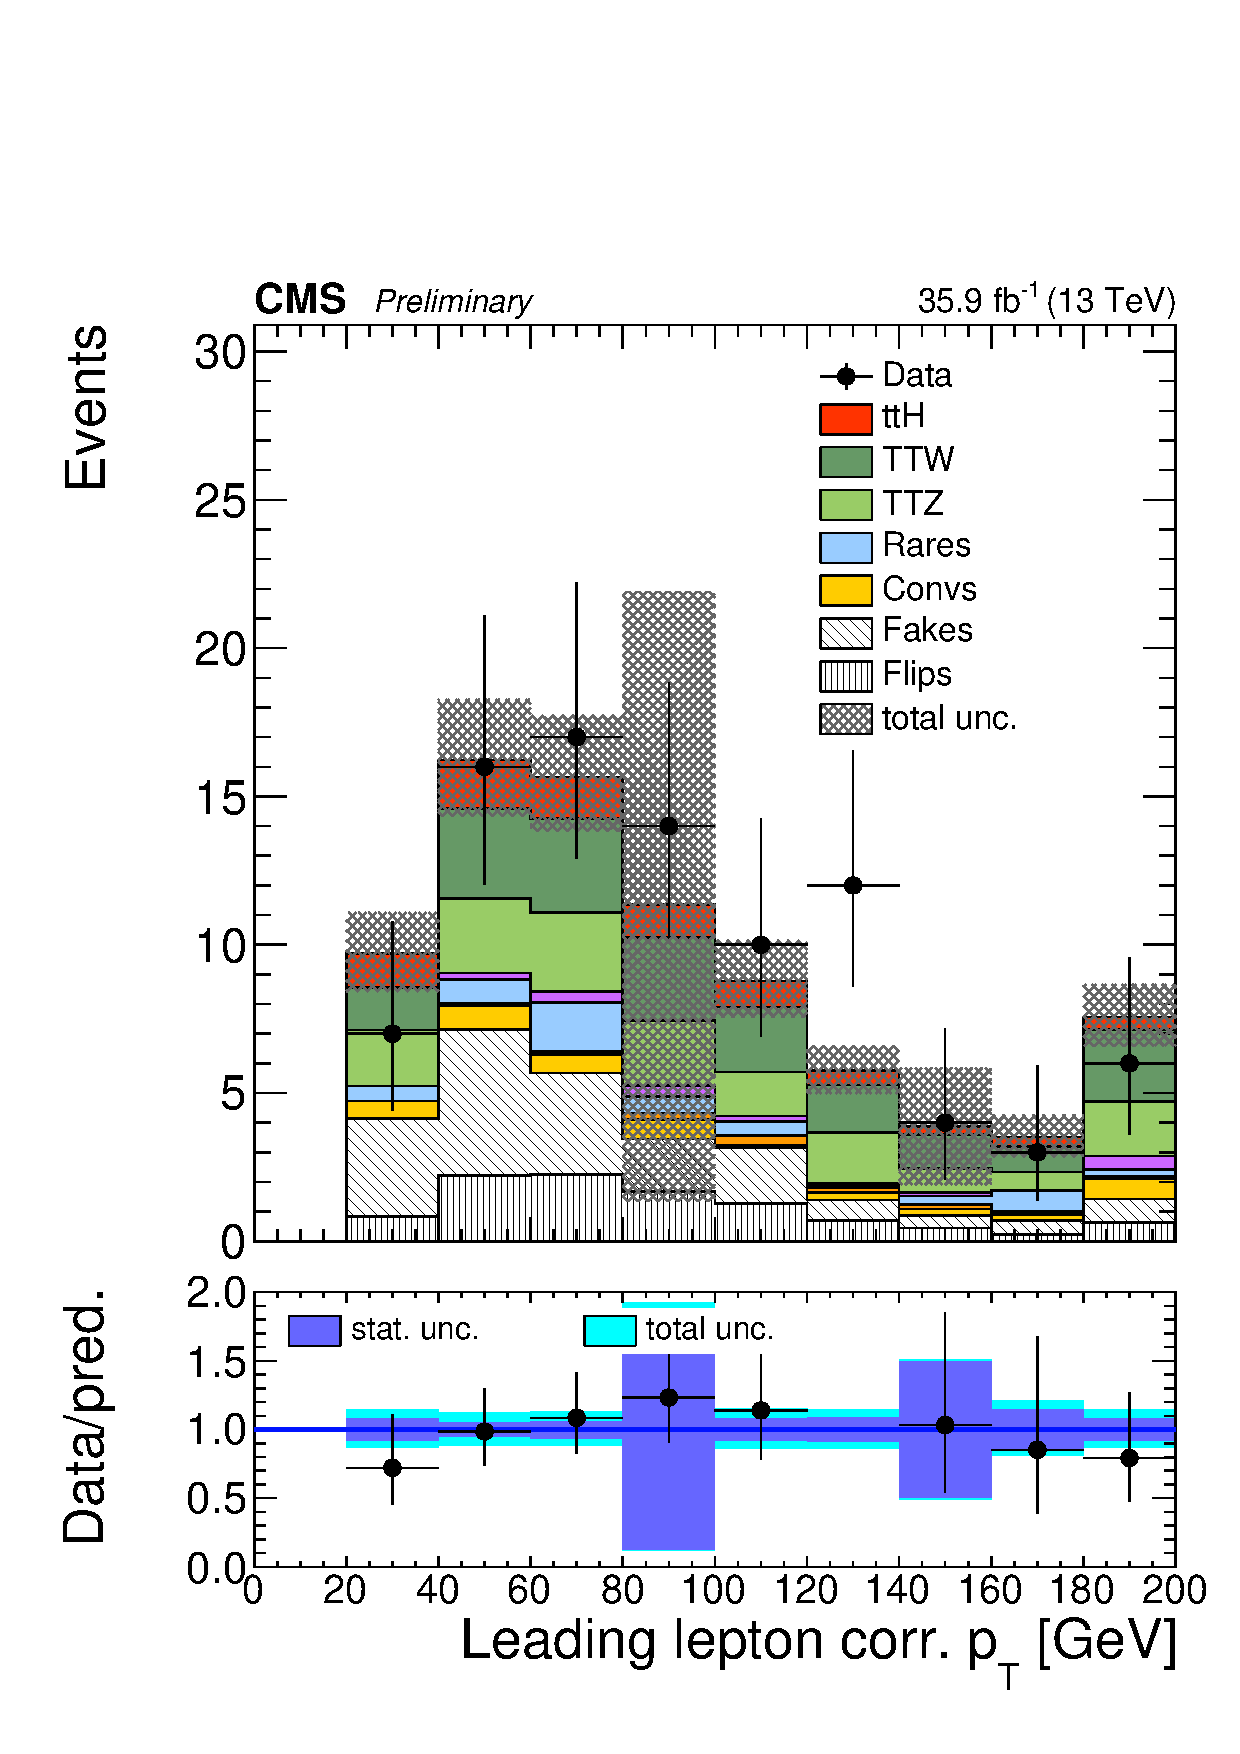
\includegraphics[width=0.32\textwidth]{plots_leptons/lep_evtsel/2lss_SR/ee/kinMVA_input_LepGood0_conePt.pdf}
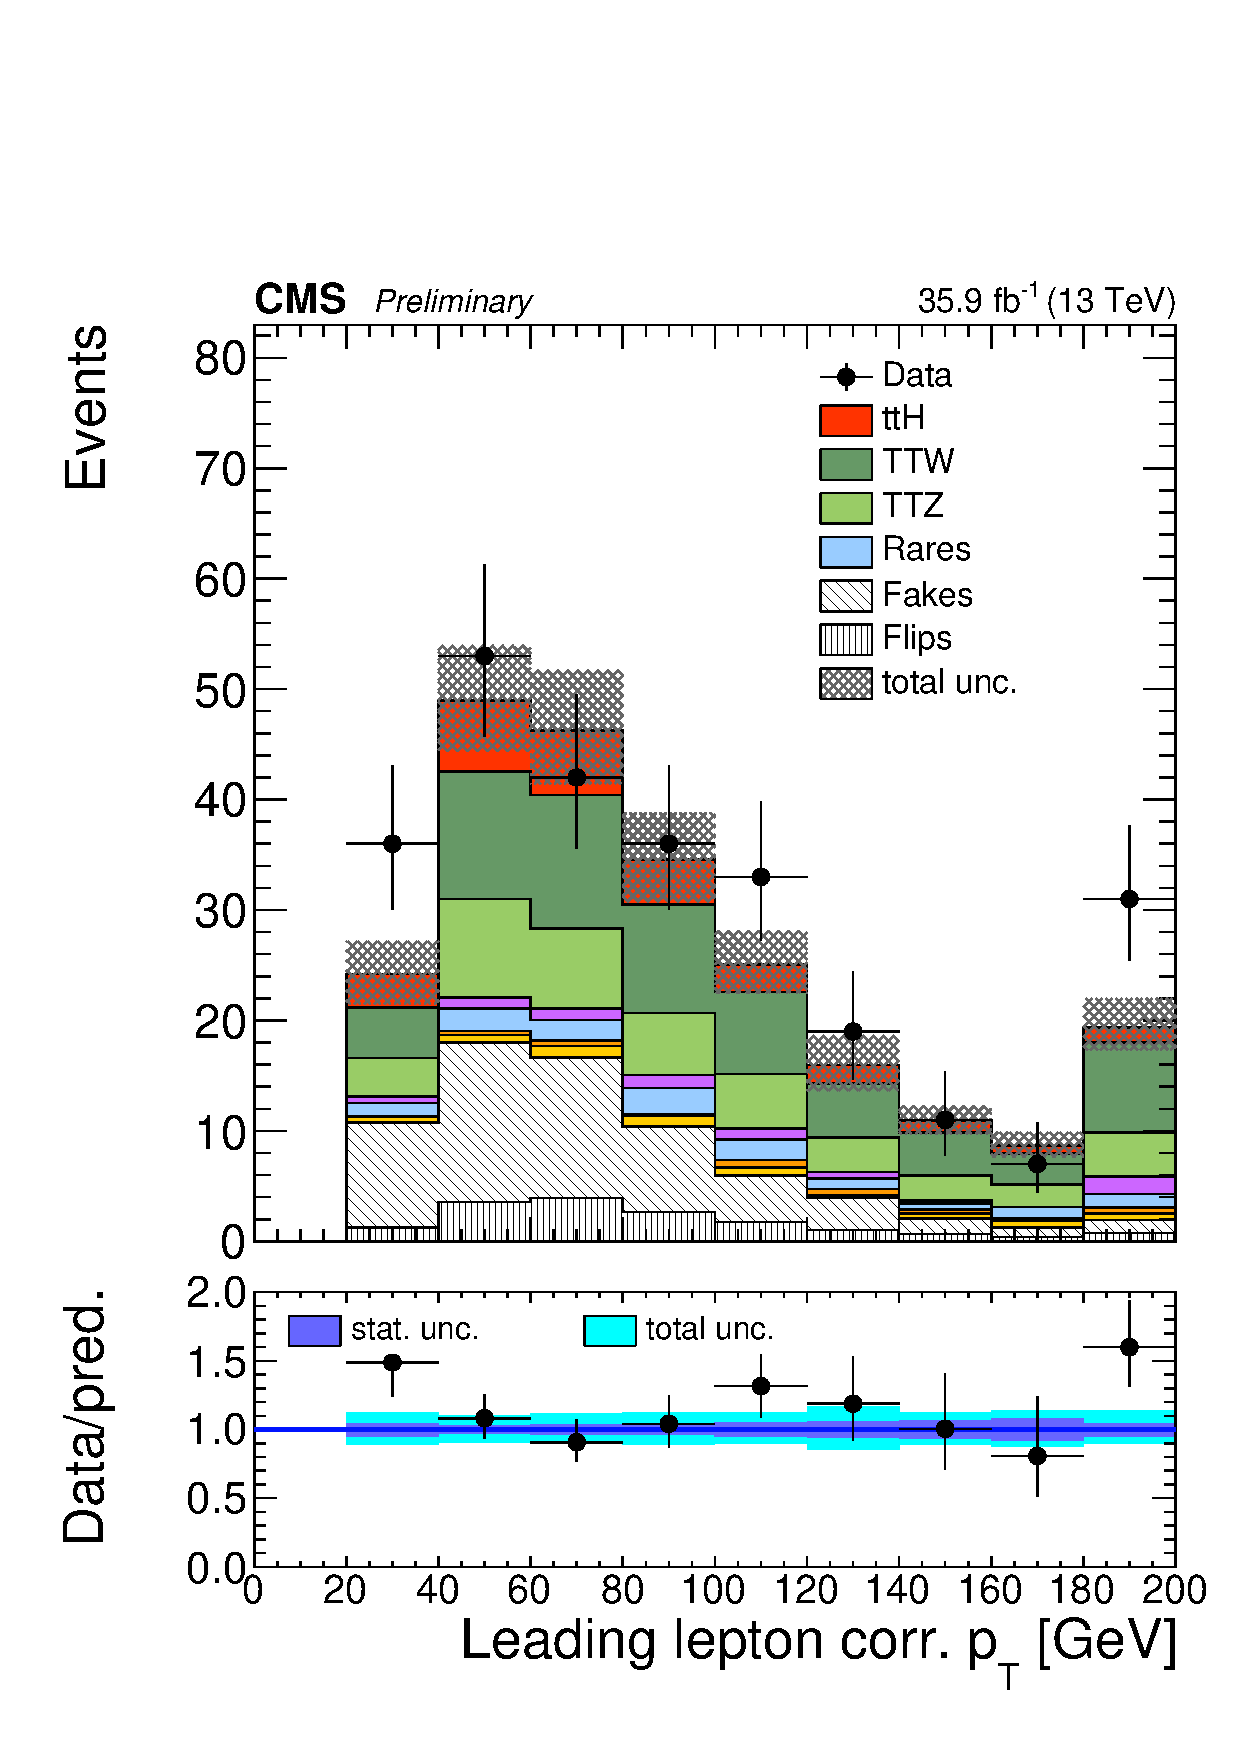
\includegraphics[width=0.32\textwidth]{plots_leptons/lep_evtsel/2lss_SR/em/kinMVA_input_LepGood0_conePt.pdf}
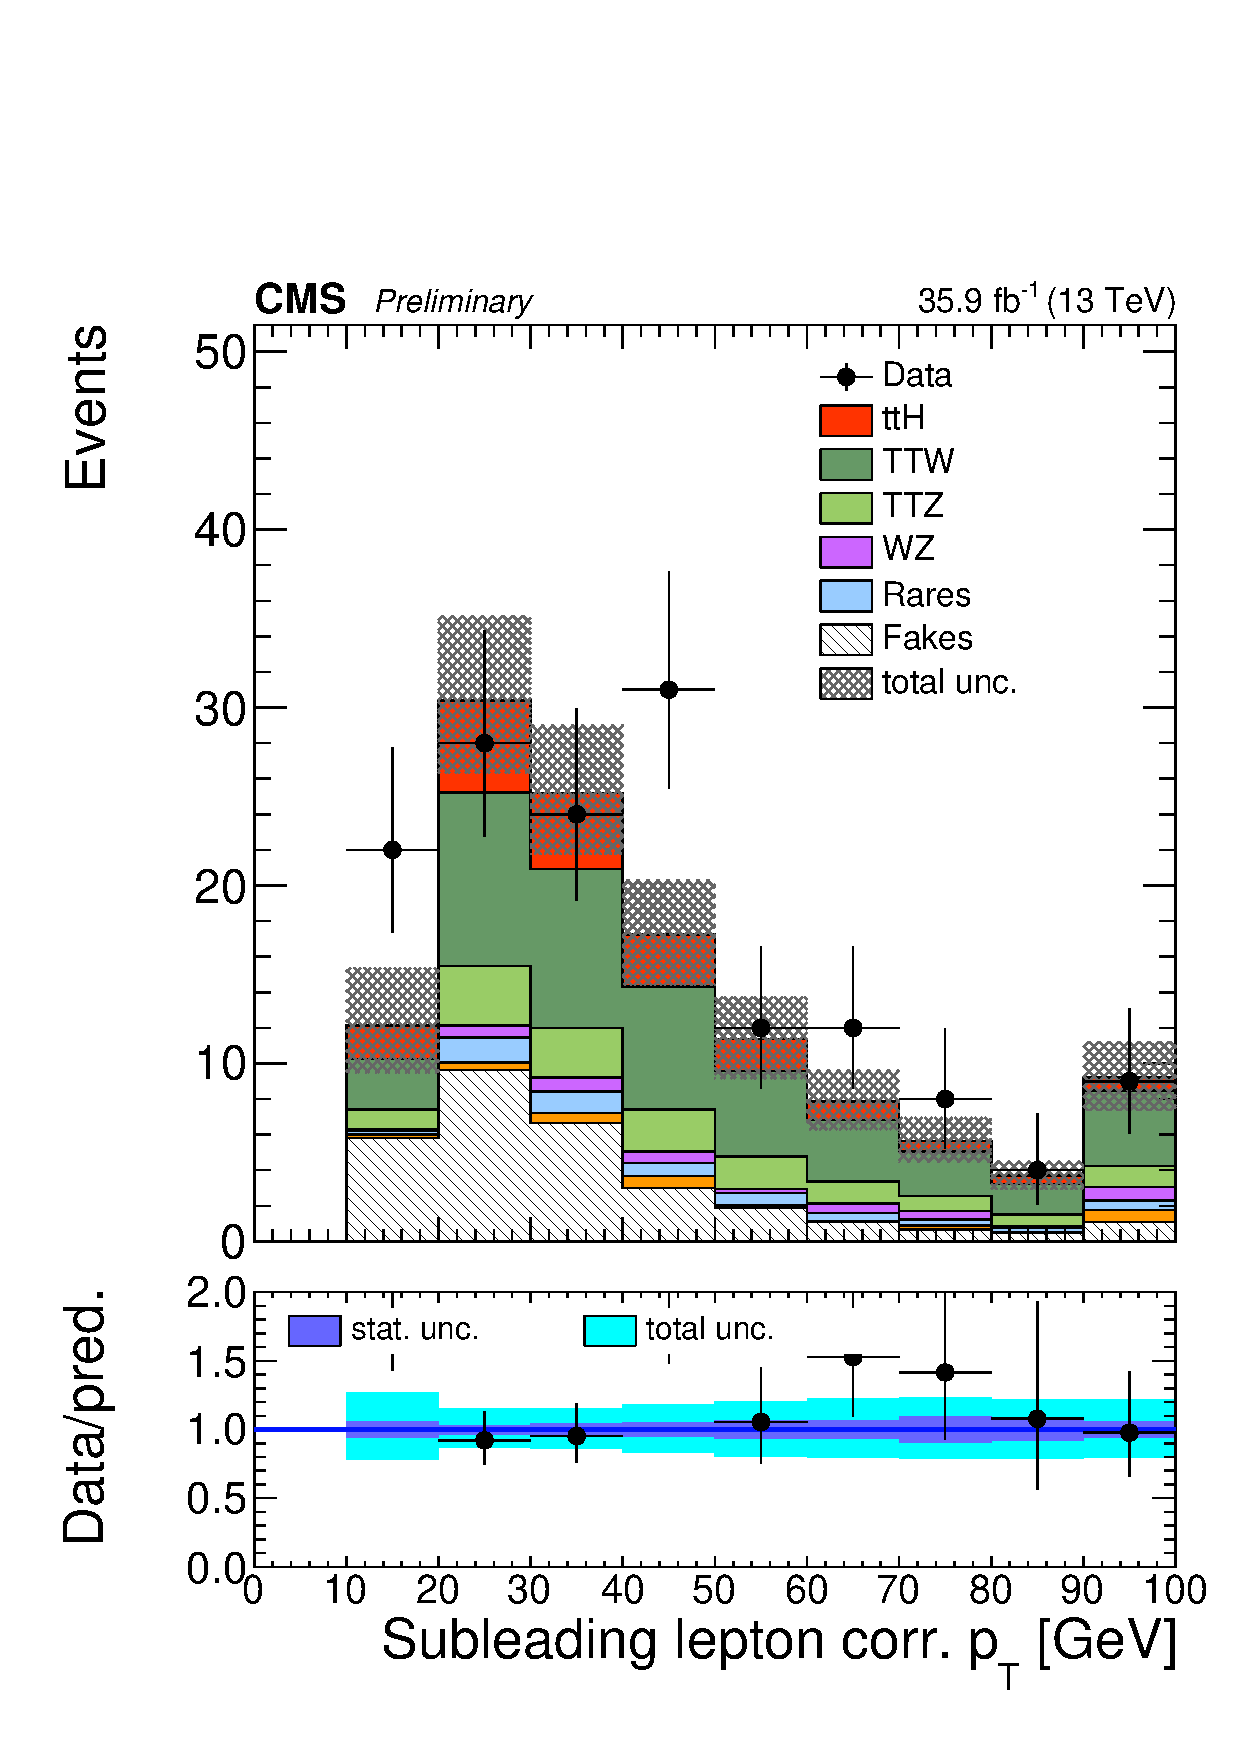
\includegraphics[width=0.32\textwidth]{plots_leptons/lep_evtsel/2lss_SR/mm/kinMVA_input_LepGood1_conePt.pdf}
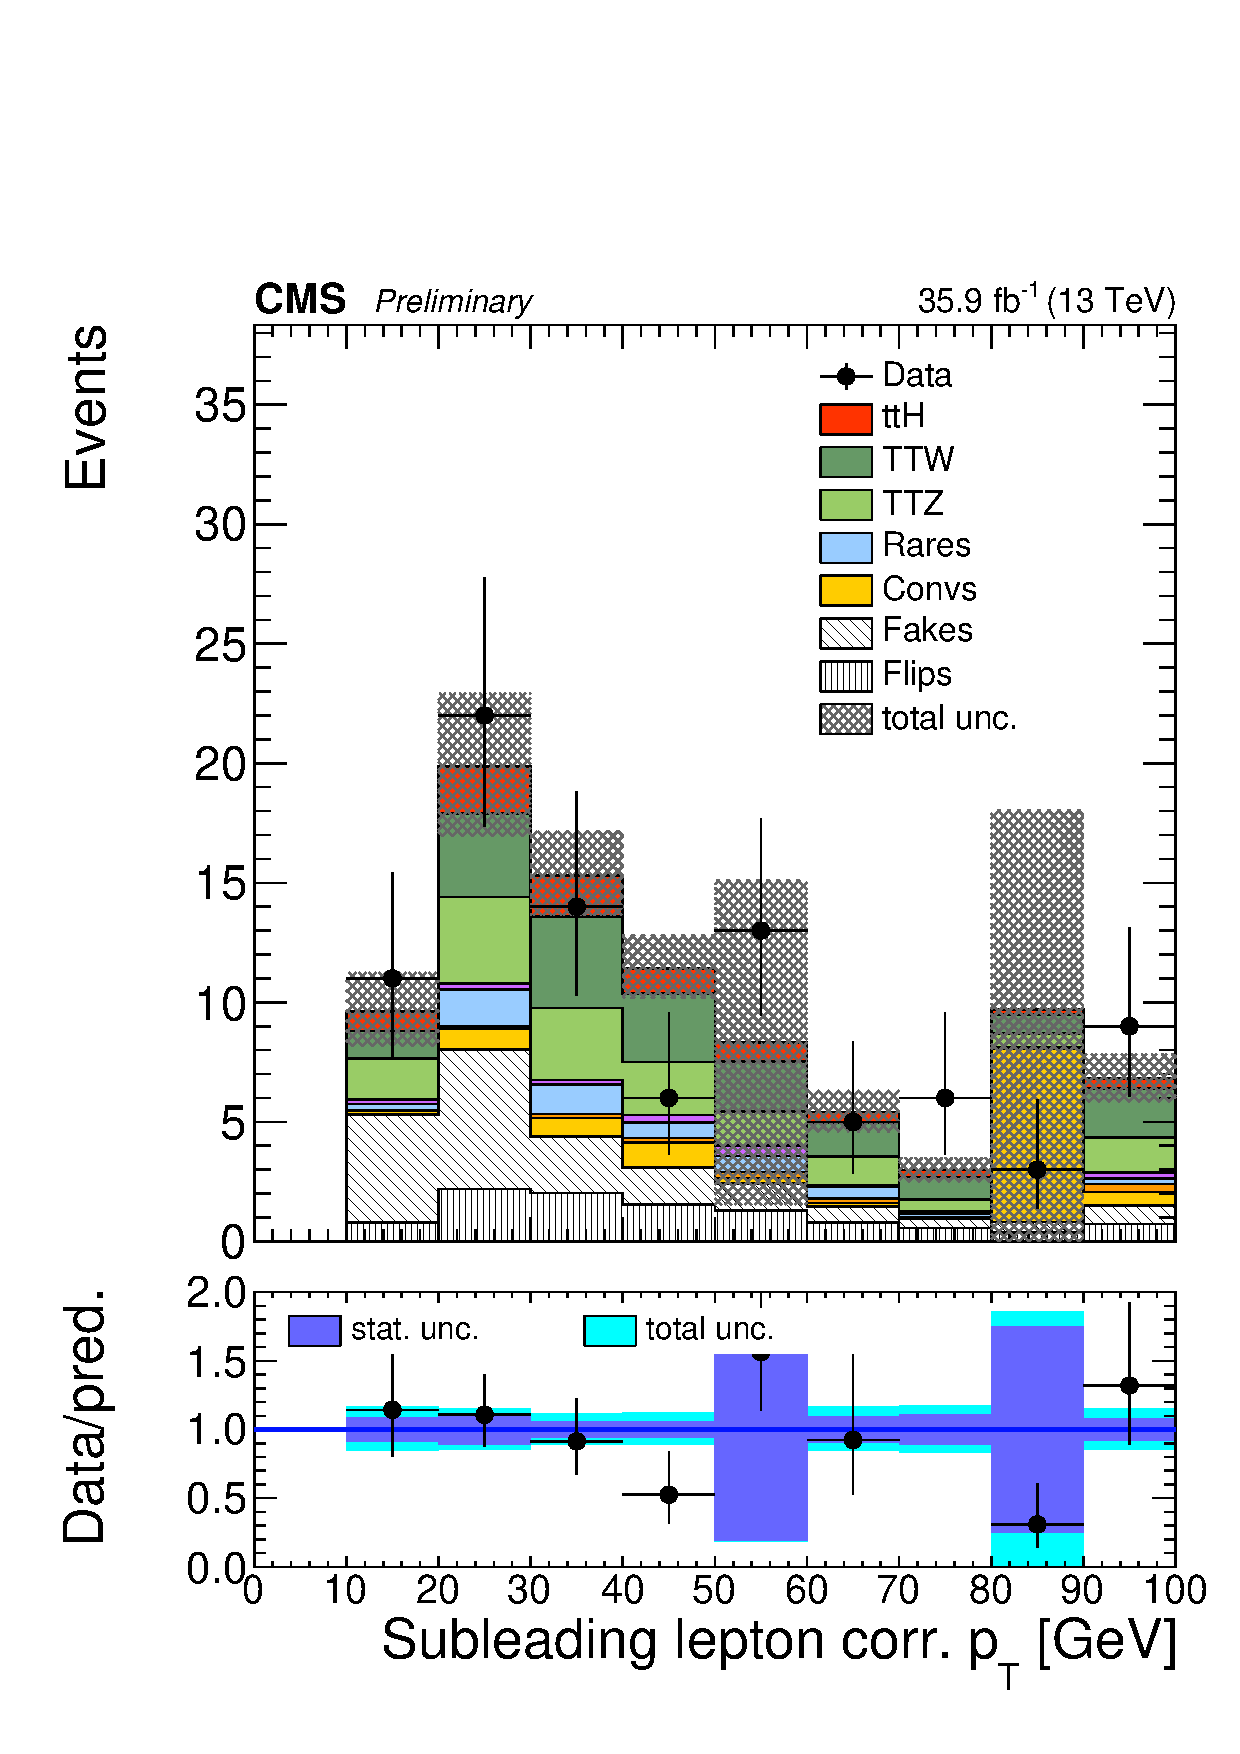
\includegraphics[width=0.32\textwidth]{plots_leptons/lep_evtsel/2lss_SR/ee/kinMVA_input_LepGood1_conePt.pdf}
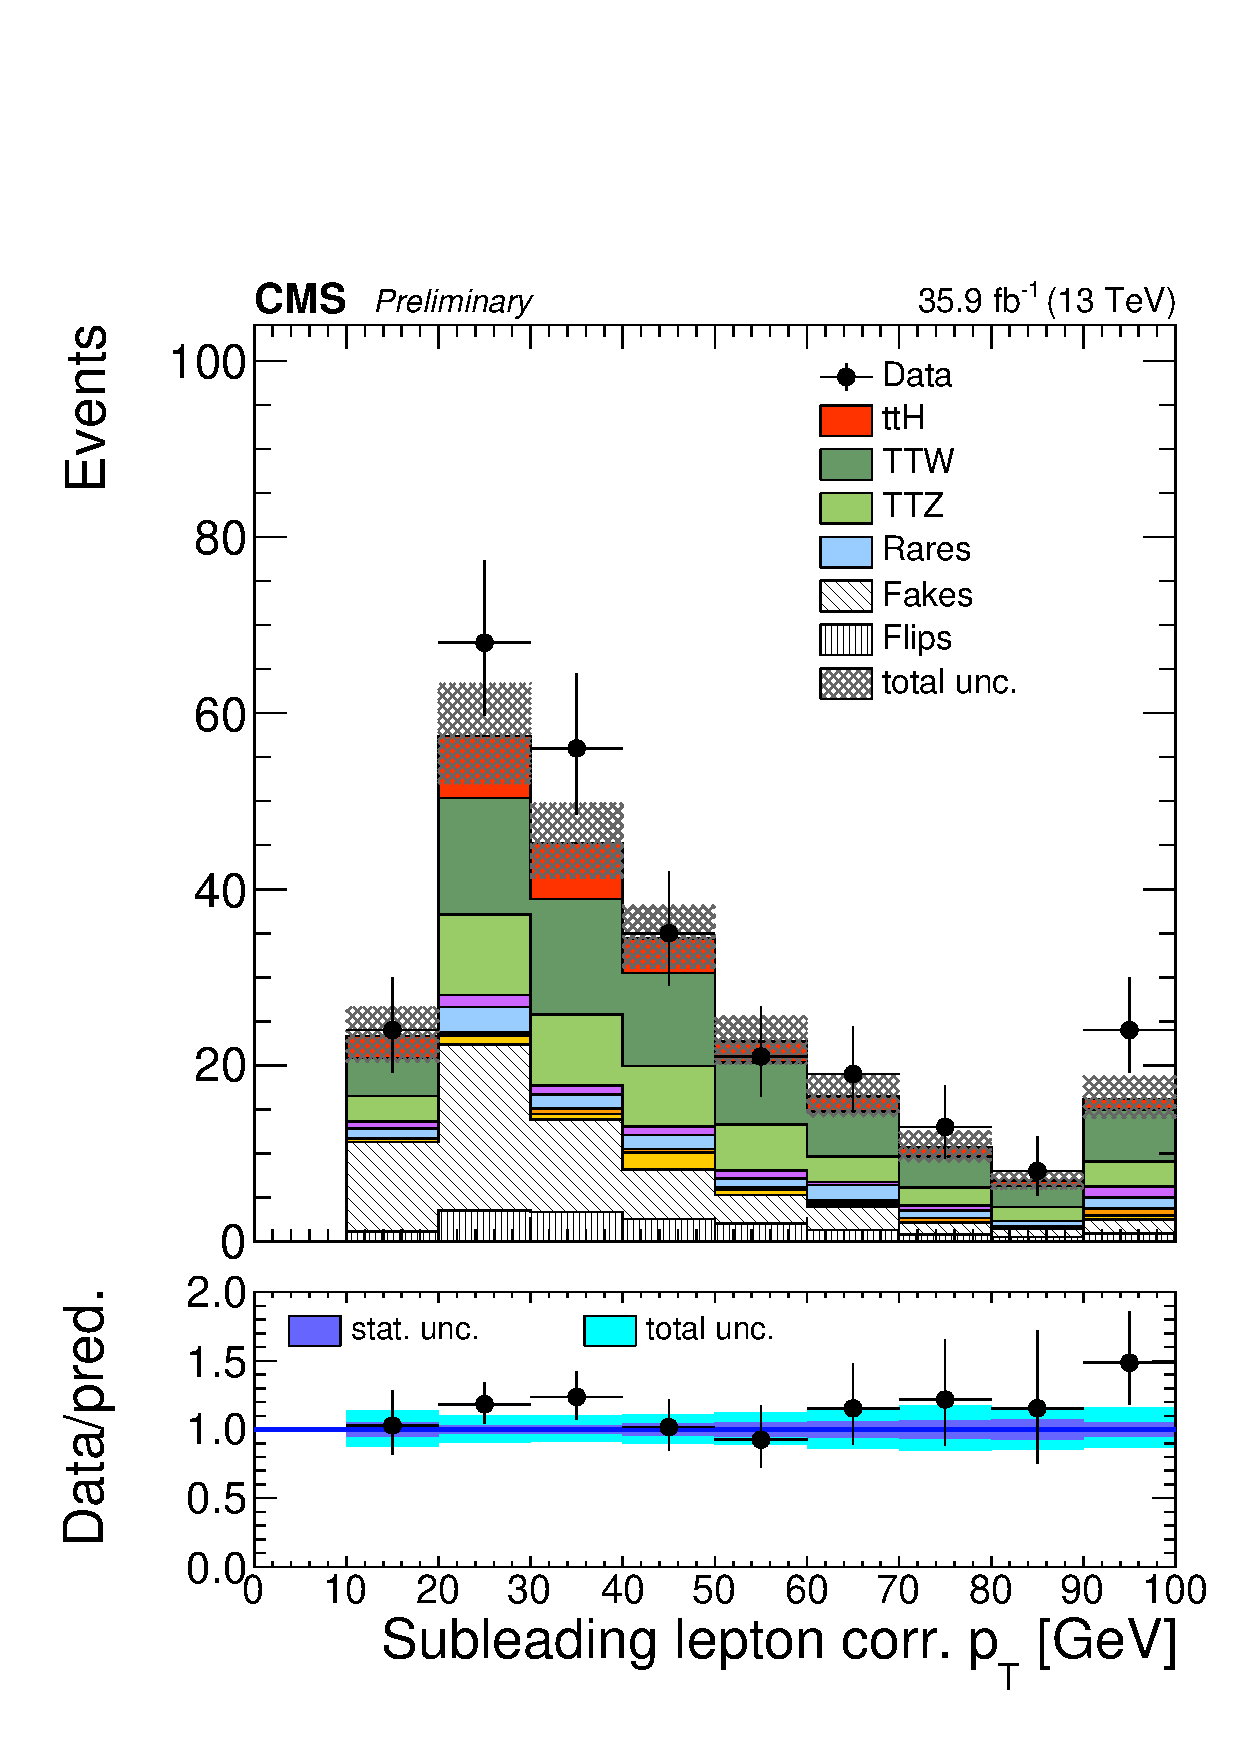
\includegraphics[width=0.32\textwidth]{plots_leptons/lep_evtsel/2lss_SR/em/kinMVA_input_LepGood1_conePt.pdf}
	\caption{Lepton transverse momentum spectra in the 2$\ell$ ($\Pgm\Pgm$, $\Pe\Pe$, $\Pe\Pgm$) selections.}
	\label{fig:2l_lepPt}
\end{figure}
\begin{figure}[htb]
	\centering 
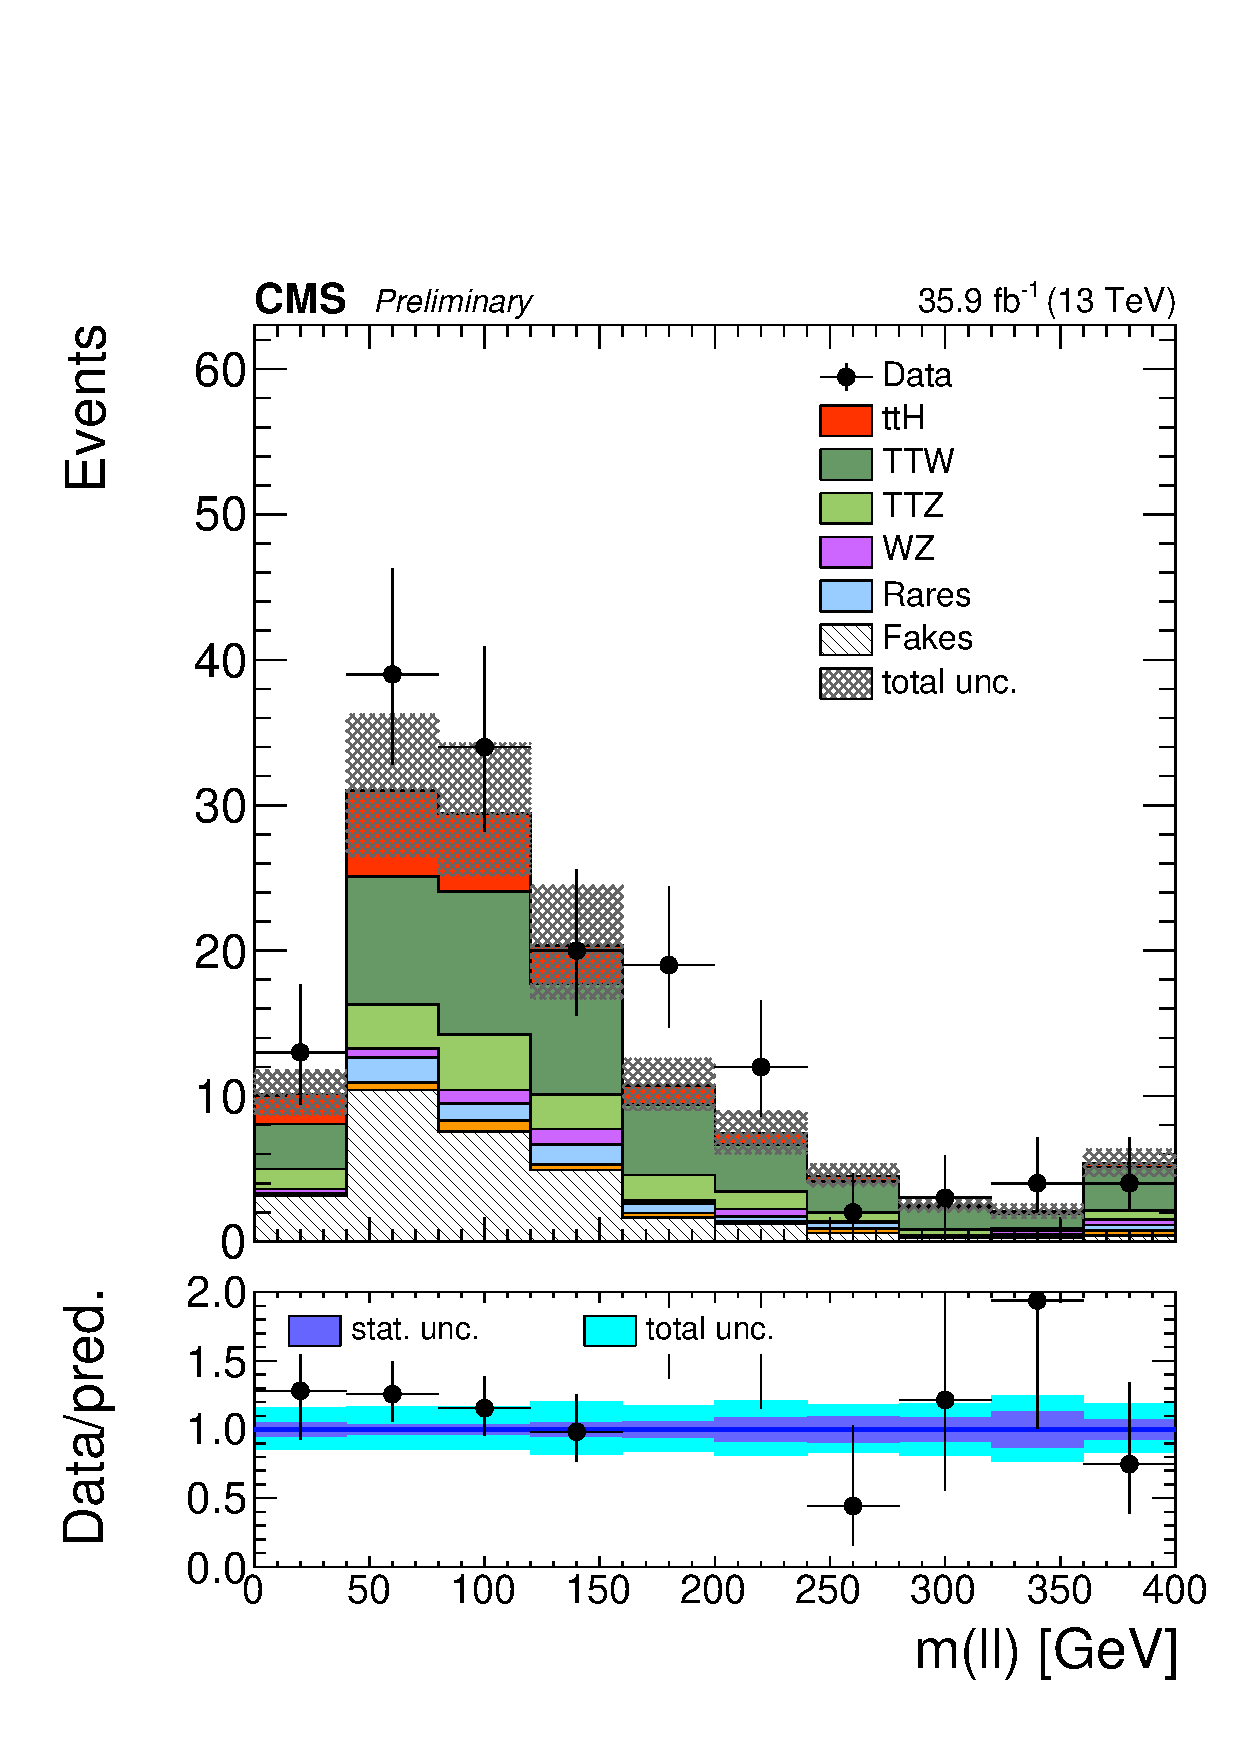
\includegraphics[width=0.32\textwidth]{plots_leptons/lep_evtsel/2lss_SR/mm/2lep_mll.pdf}
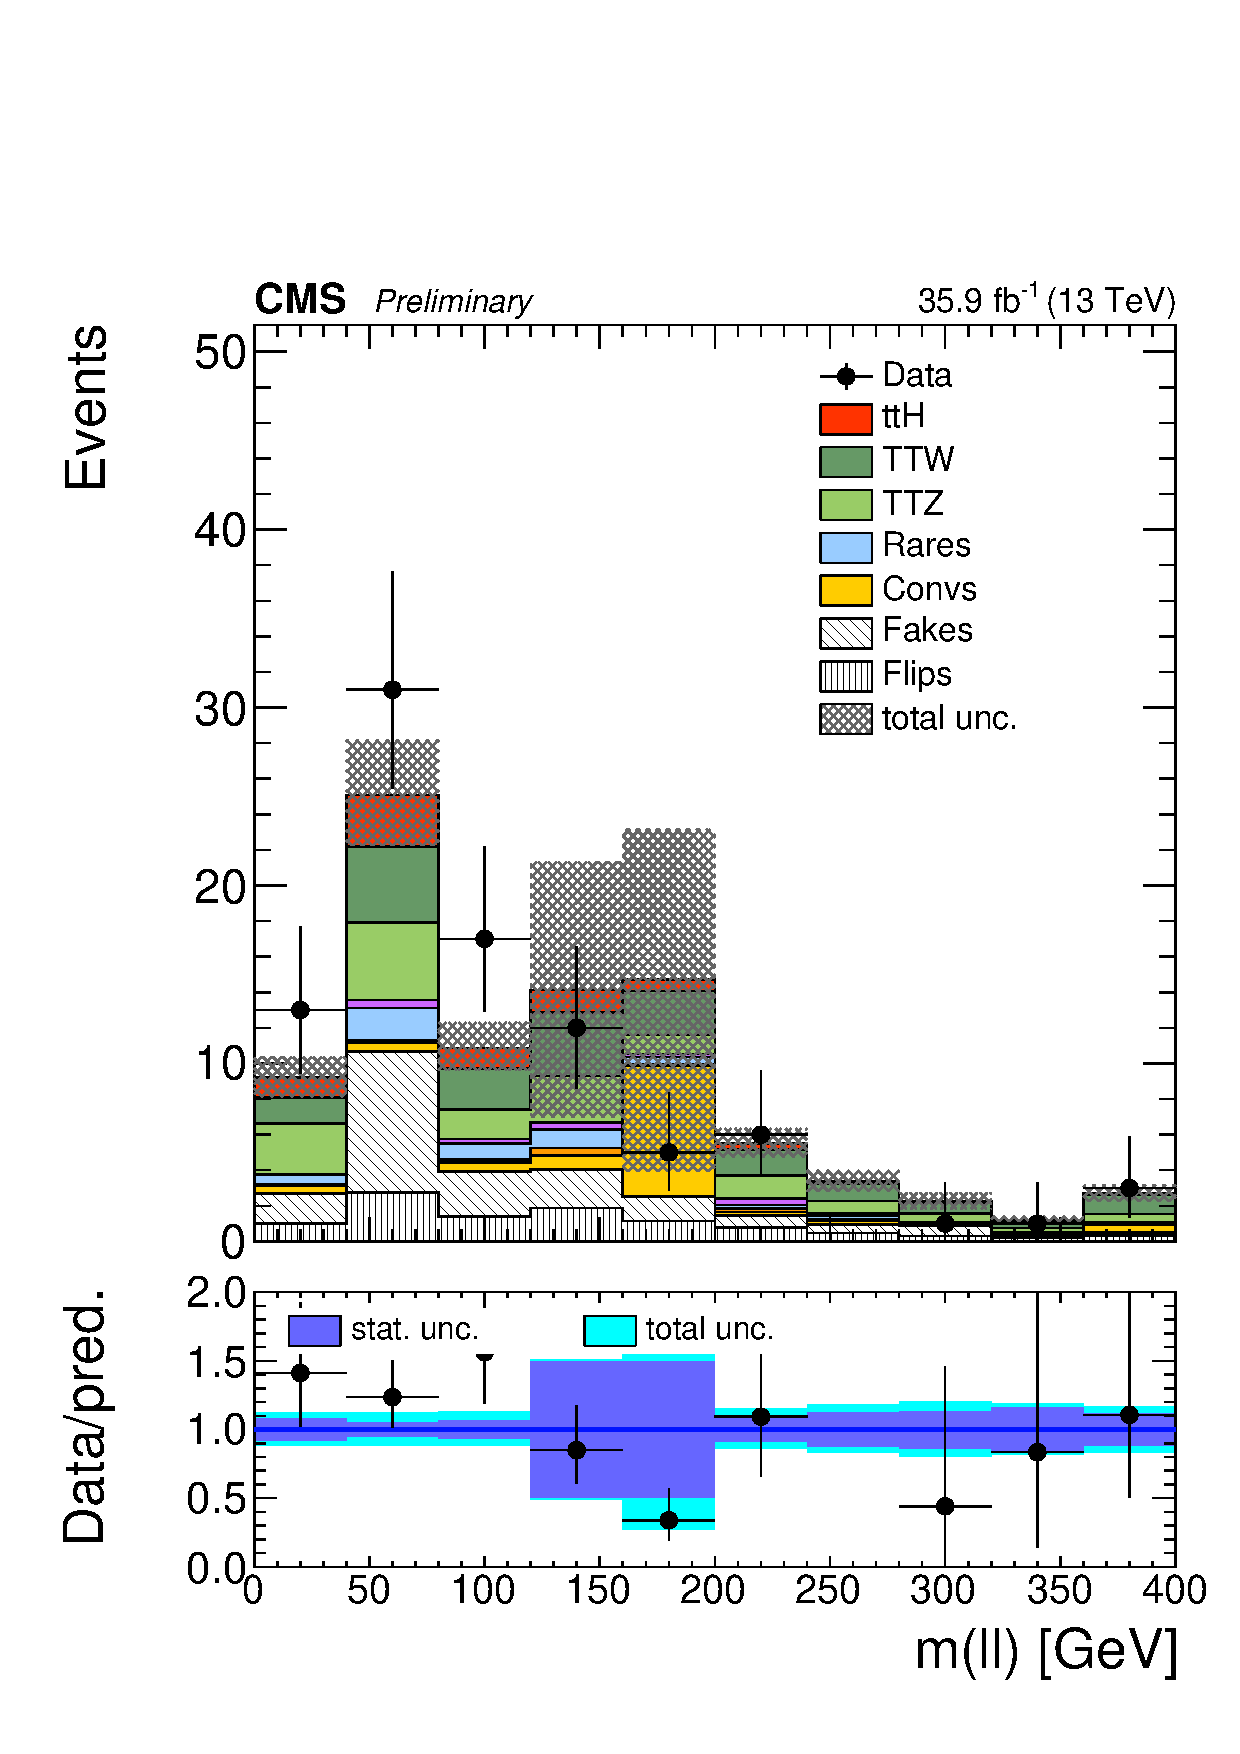
\includegraphics[width=0.32\textwidth]{plots_leptons/lep_evtsel/2lss_SR/ee/2lep_mll.pdf}
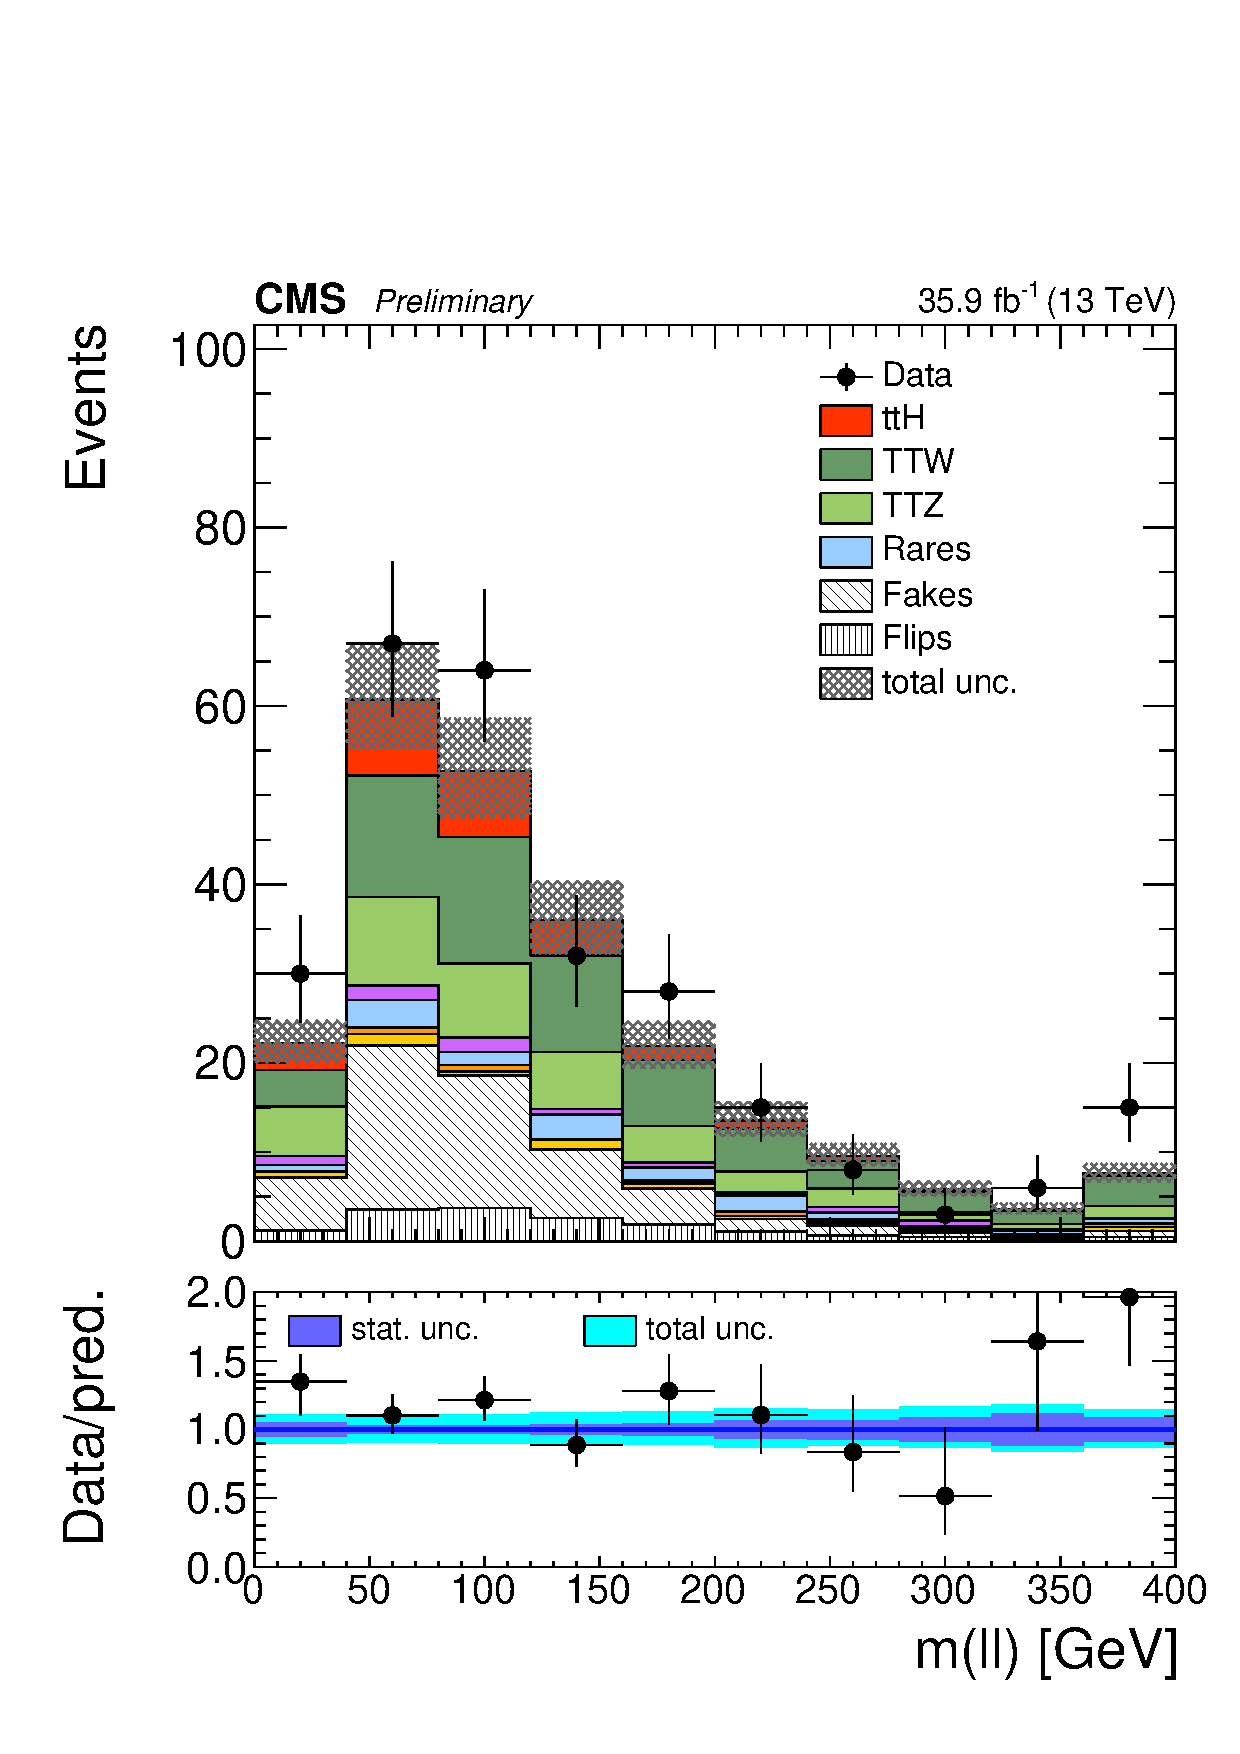
\includegraphics[width=0.32\textwidth]{plots_leptons/lep_evtsel/2lss_SR/em/2lep_mll.pdf}
	\caption{Di-lepton invariant mass spectra in the 2$\ell$ ($\Pgm\Pgm$, $\Pe\Pe$, $\Pe\Pgm$) selections.}
	\label{fig:2l_mll}
\end{figure}

\begin{figure}[htb]
	\centering 
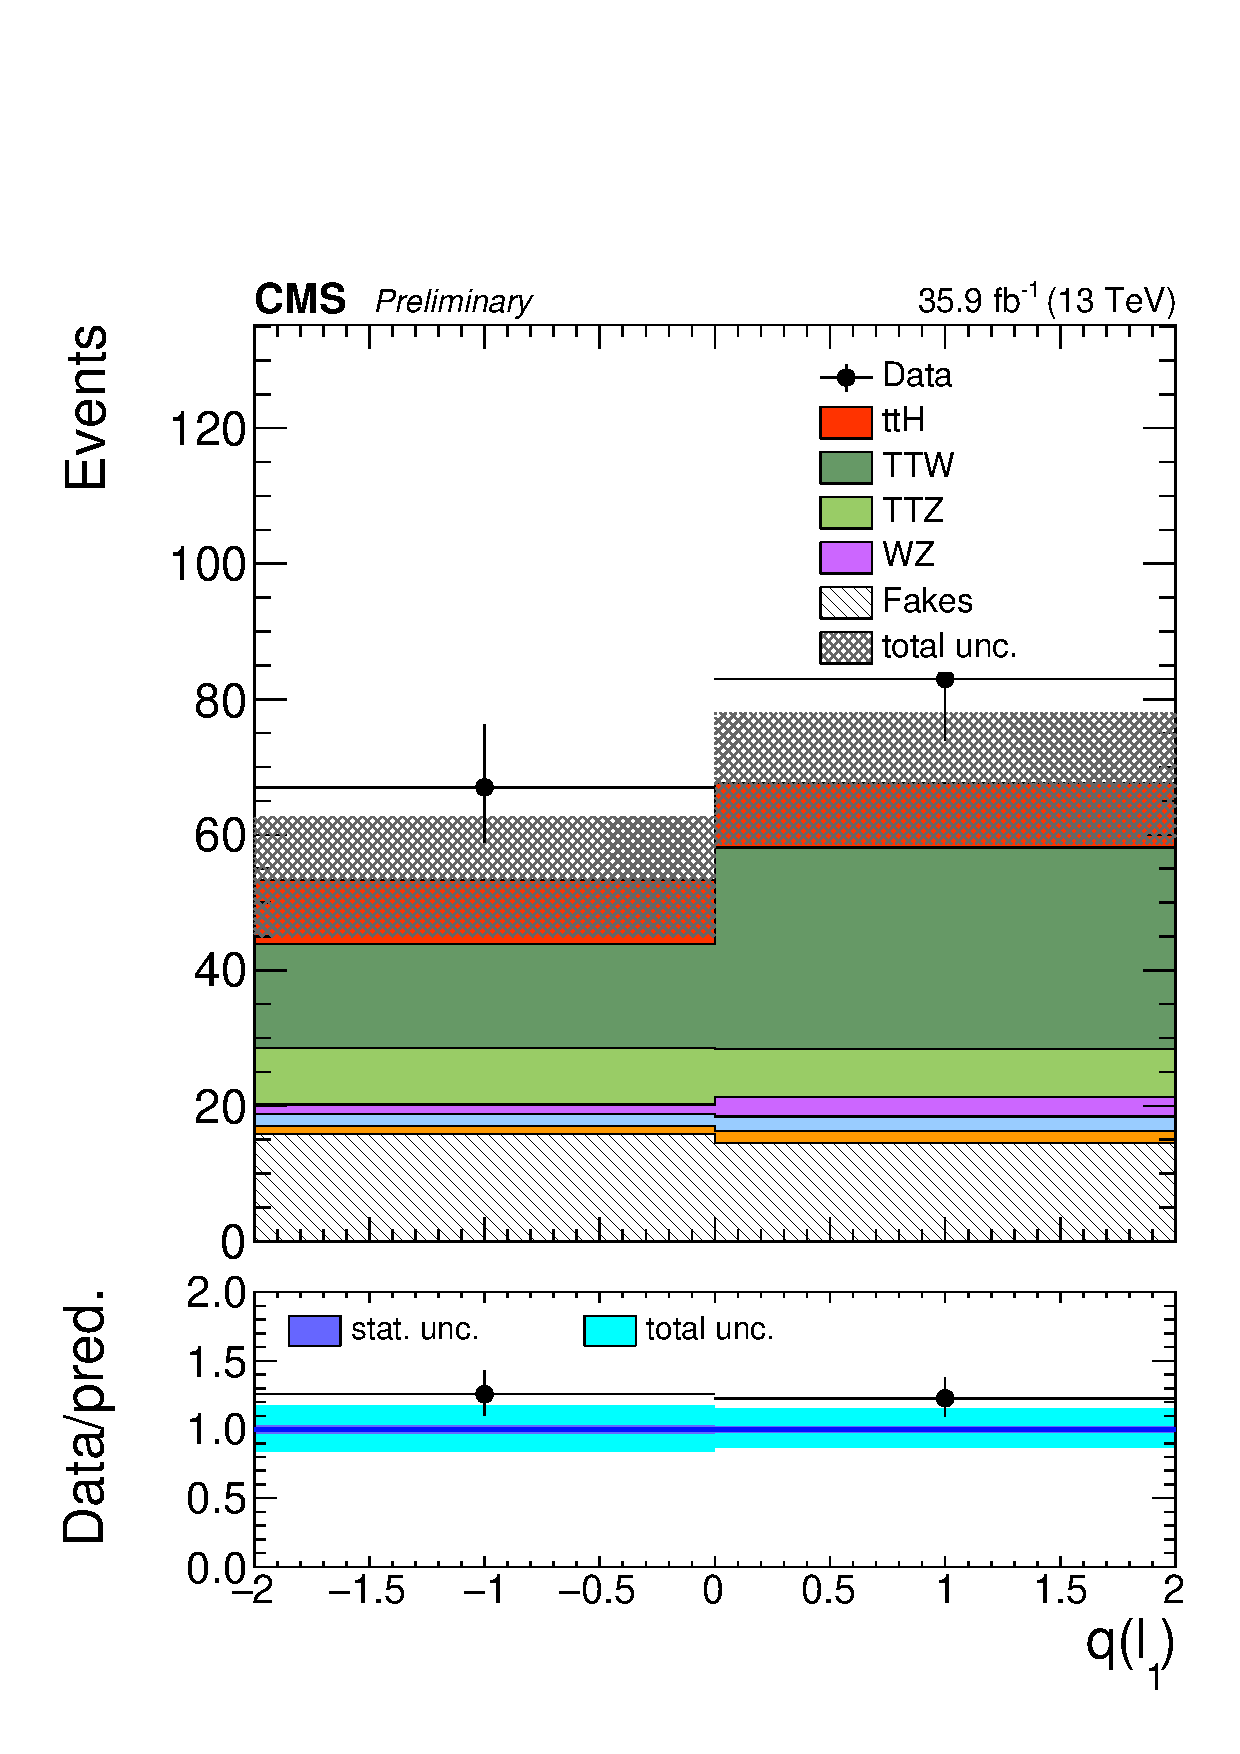
\includegraphics[width=0.32\textwidth]{plots_leptons/lep_evtsel/2lss_SR/mm/2lep_charge.pdf}
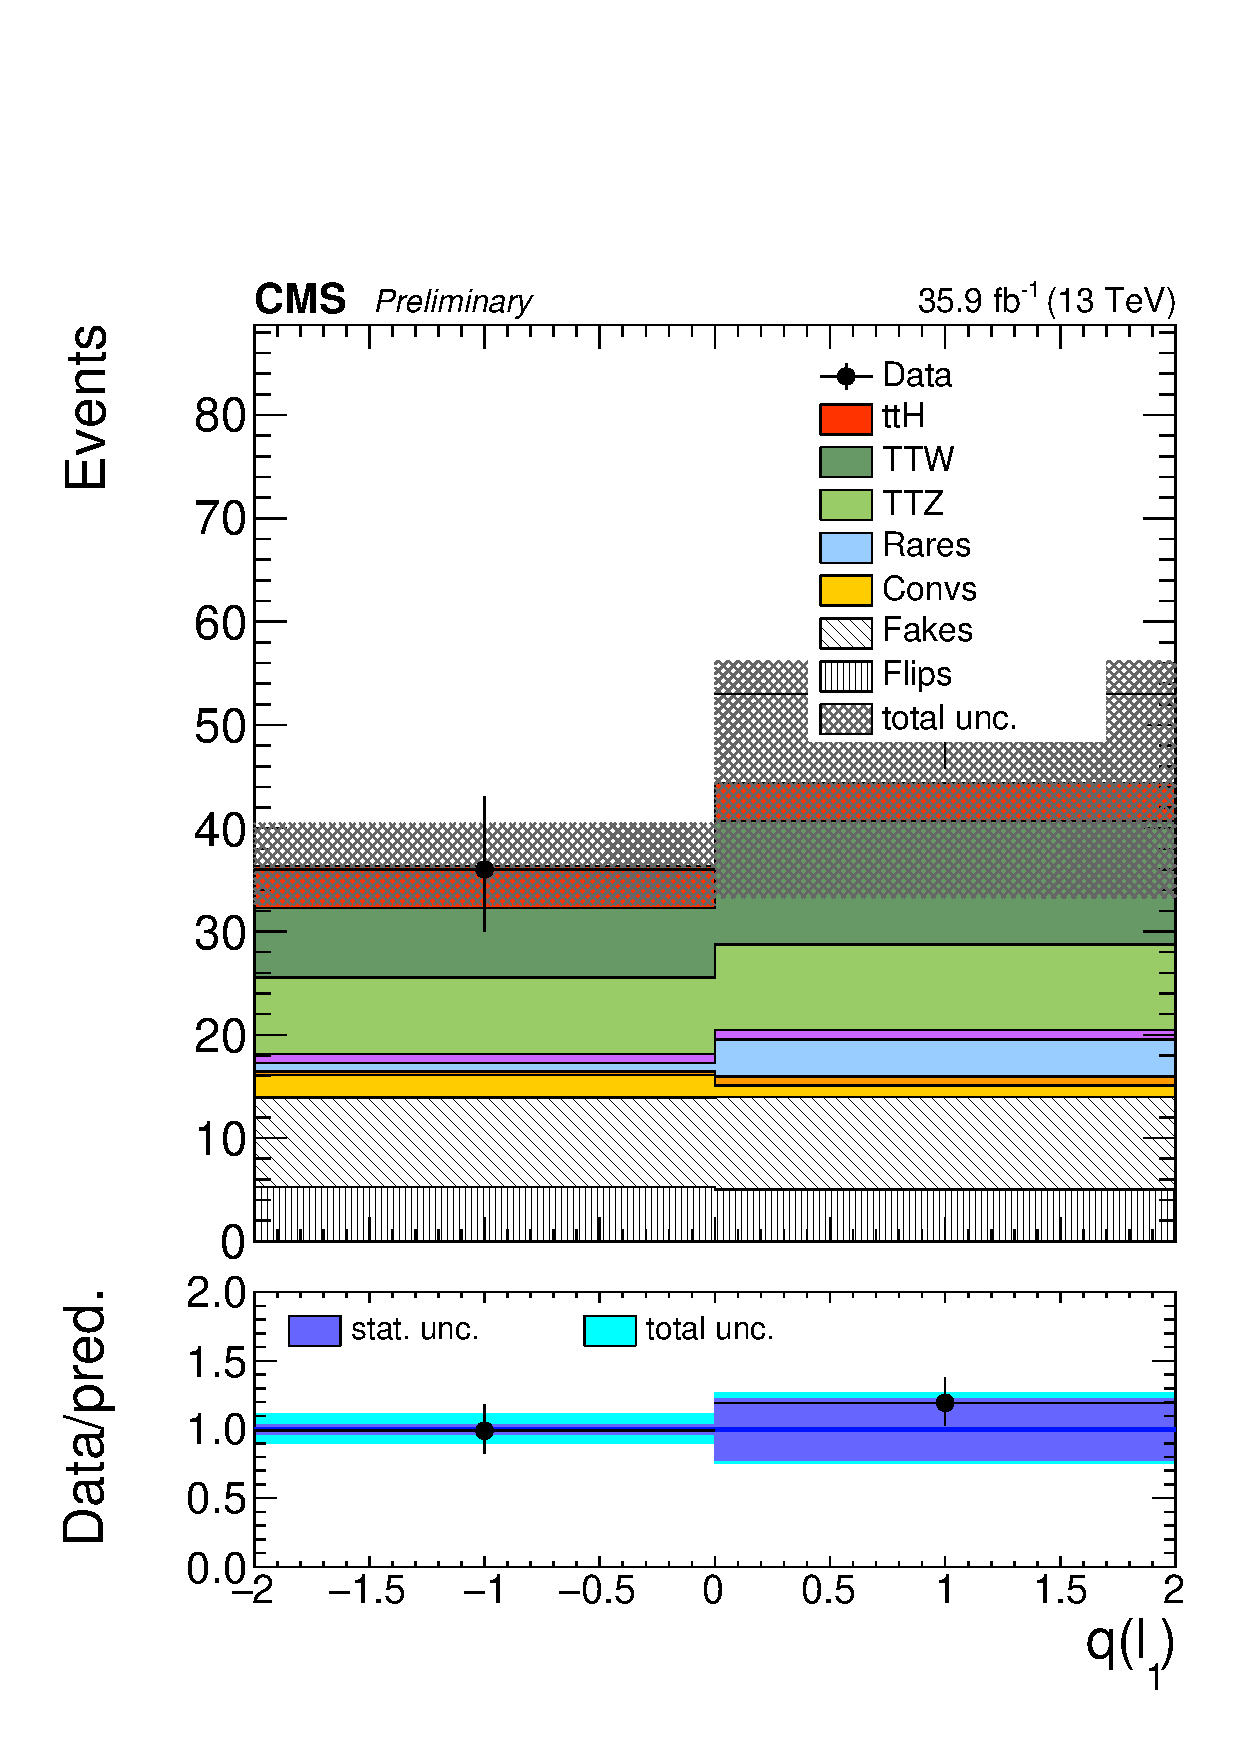
\includegraphics[width=0.32\textwidth]{plots_leptons/lep_evtsel/2lss_SR/ee/2lep_charge.pdf}
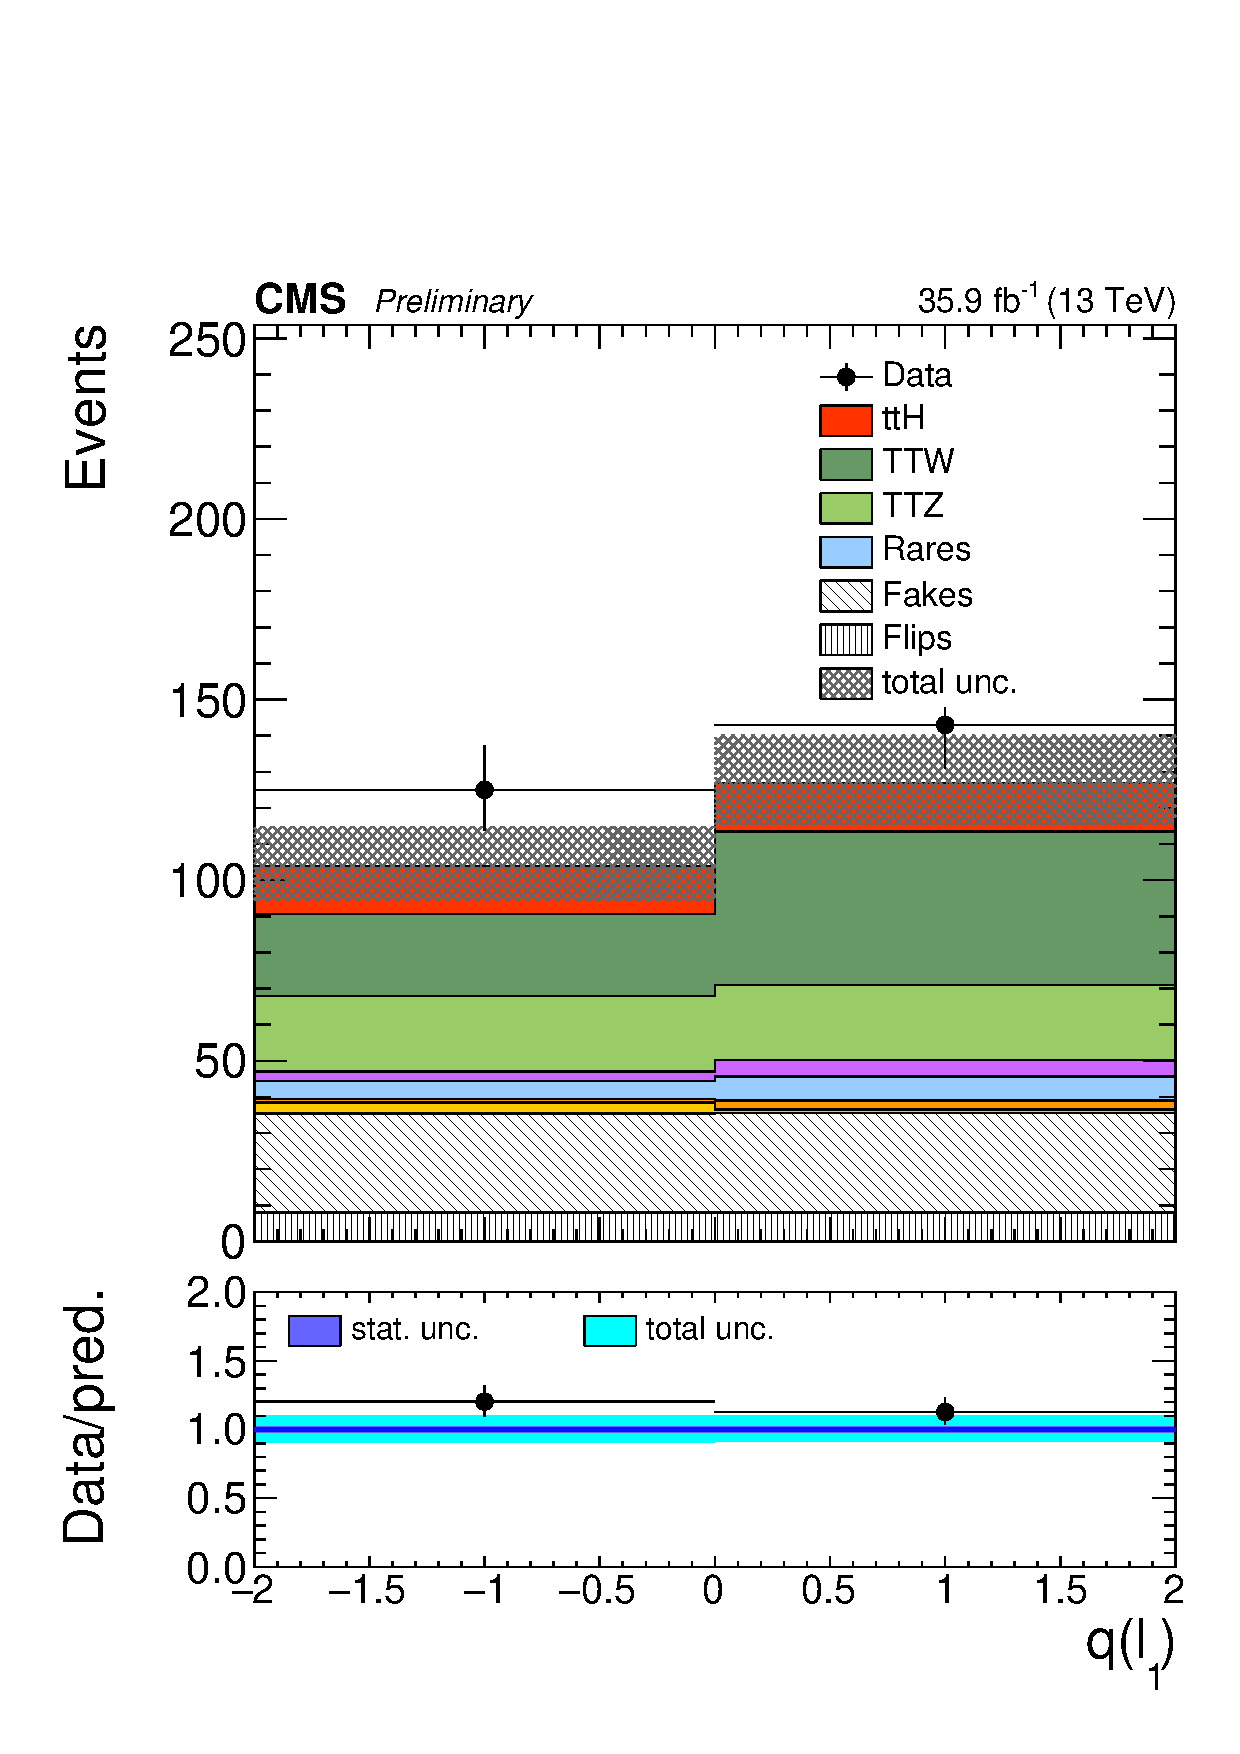
\includegraphics[width=0.32\textwidth]{plots_leptons/lep_evtsel/2lss_SR/em/2lep_charge.pdf}
	\caption{Sum of lepton charges in the 2$\ell$ ($\Pgm\Pgm$, $\Pe\Pe$, $\Pe\Pgm$) selections.}
	\label{fig:2l_charge}
\end{figure}


\begin{figure}[htb]
	\centering 
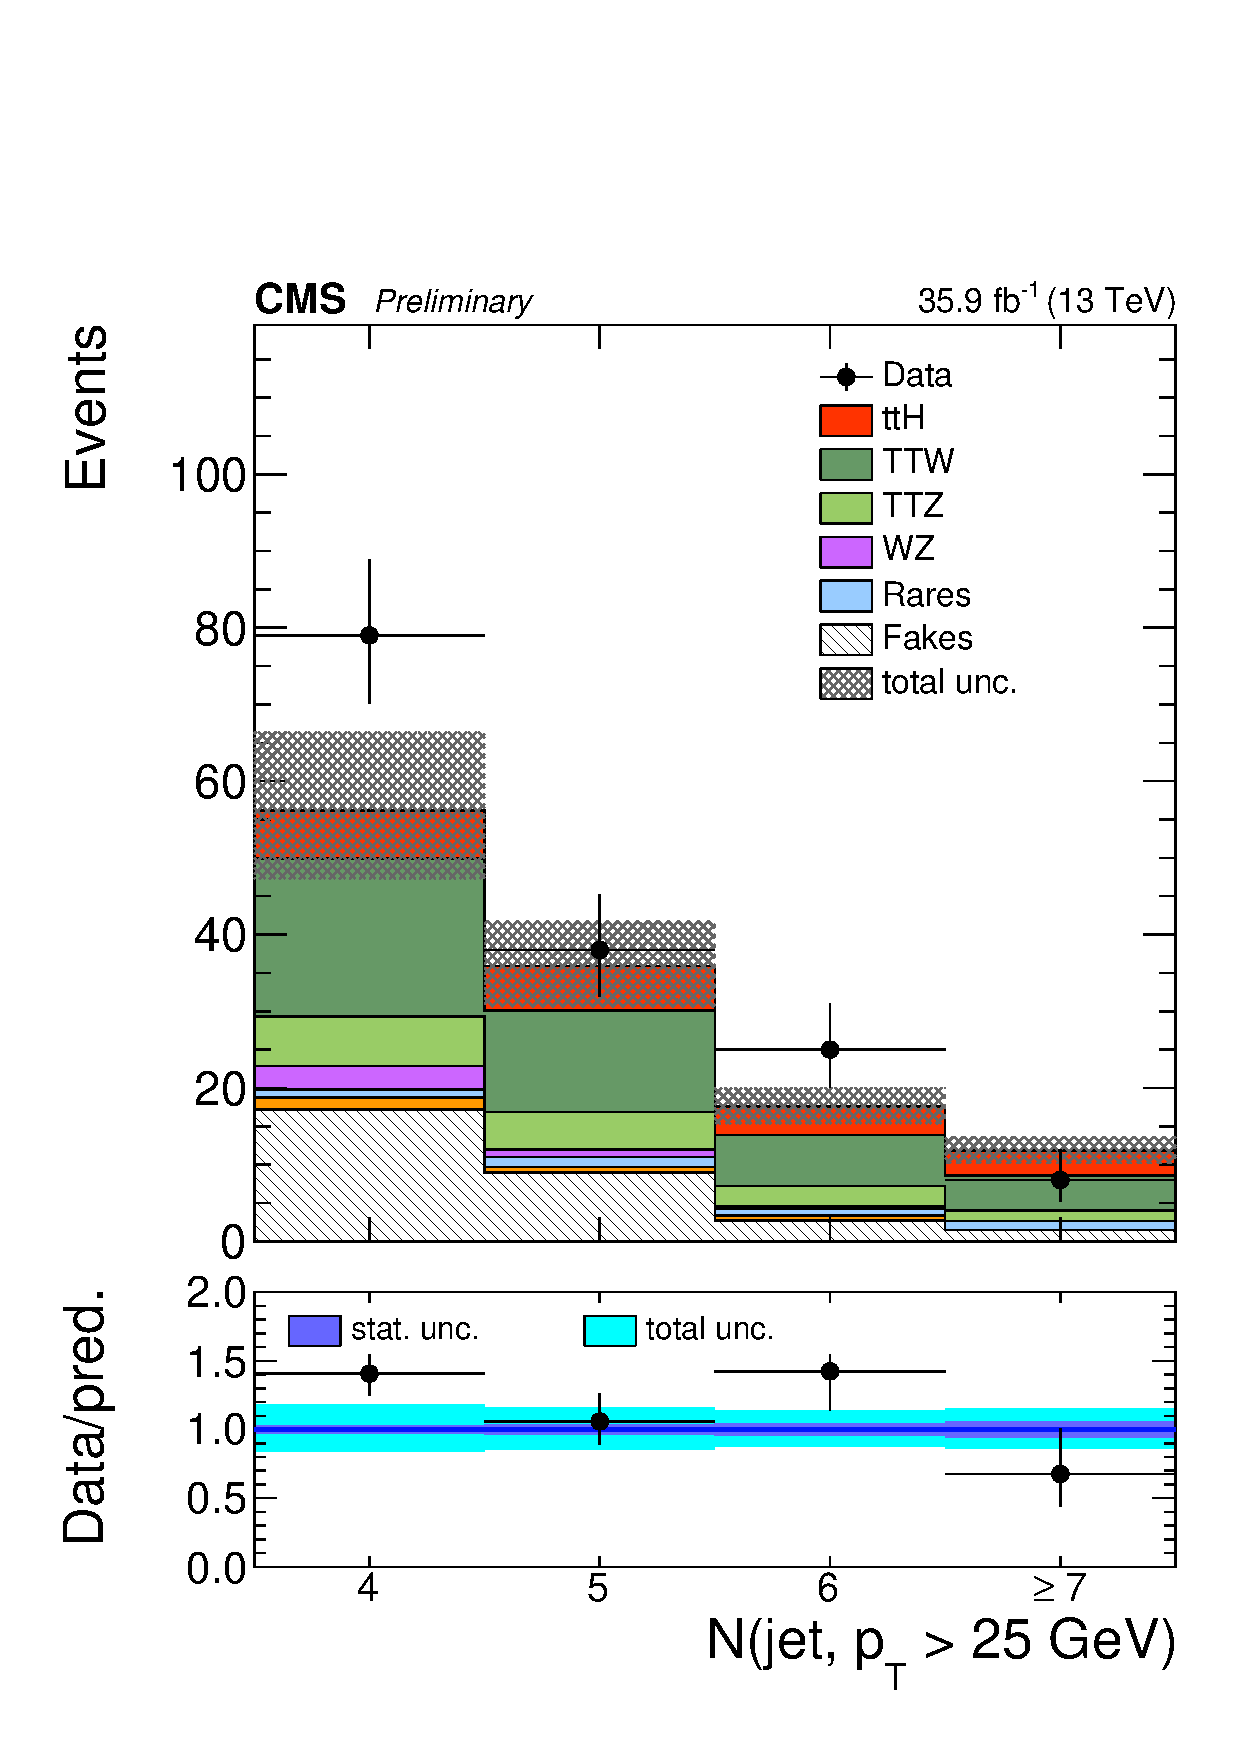
\includegraphics[width=0.32\textwidth]{plots_leptons/lep_evtsel/2lss_SR/mm/2lep_nJet25_from4.pdf}
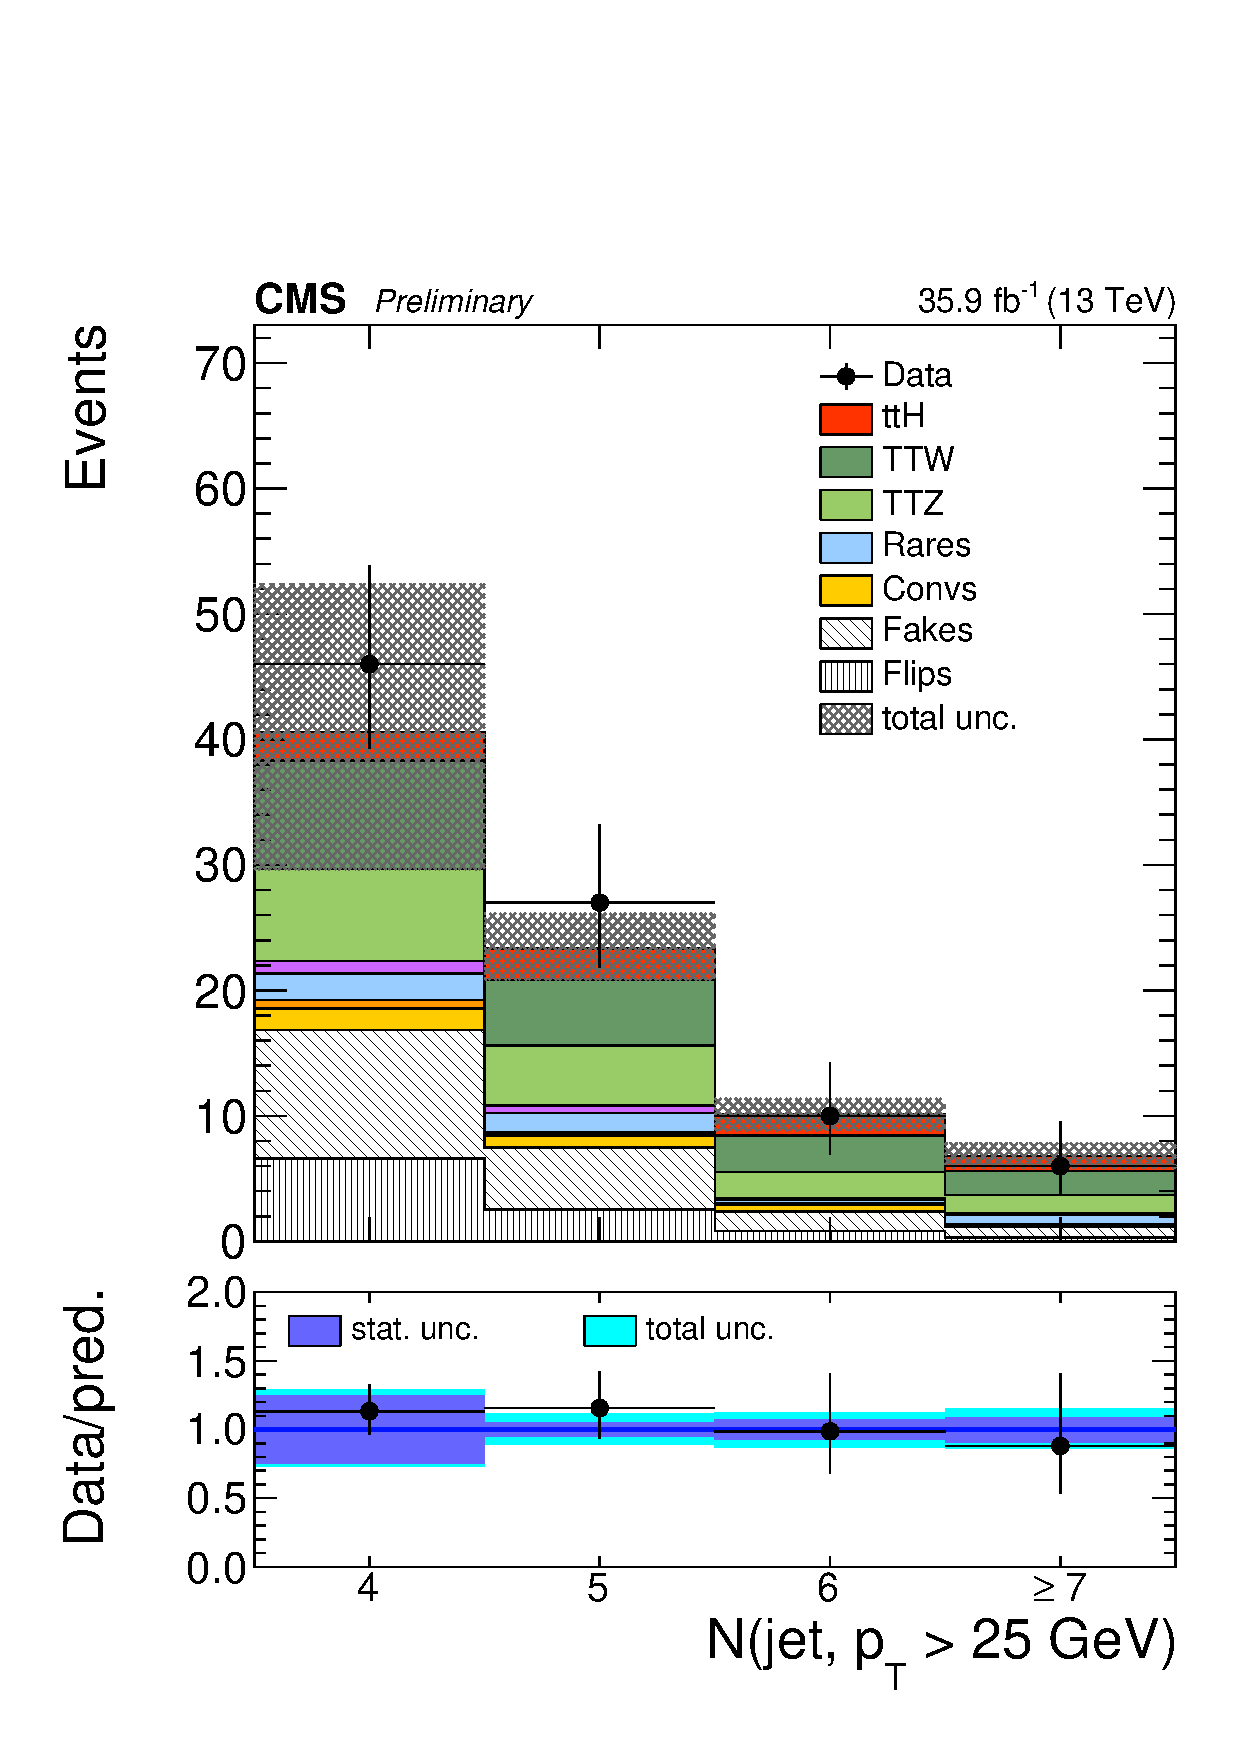
\includegraphics[width=0.32\textwidth]{plots_leptons/lep_evtsel/2lss_SR/ee/2lep_nJet25_from4.pdf}
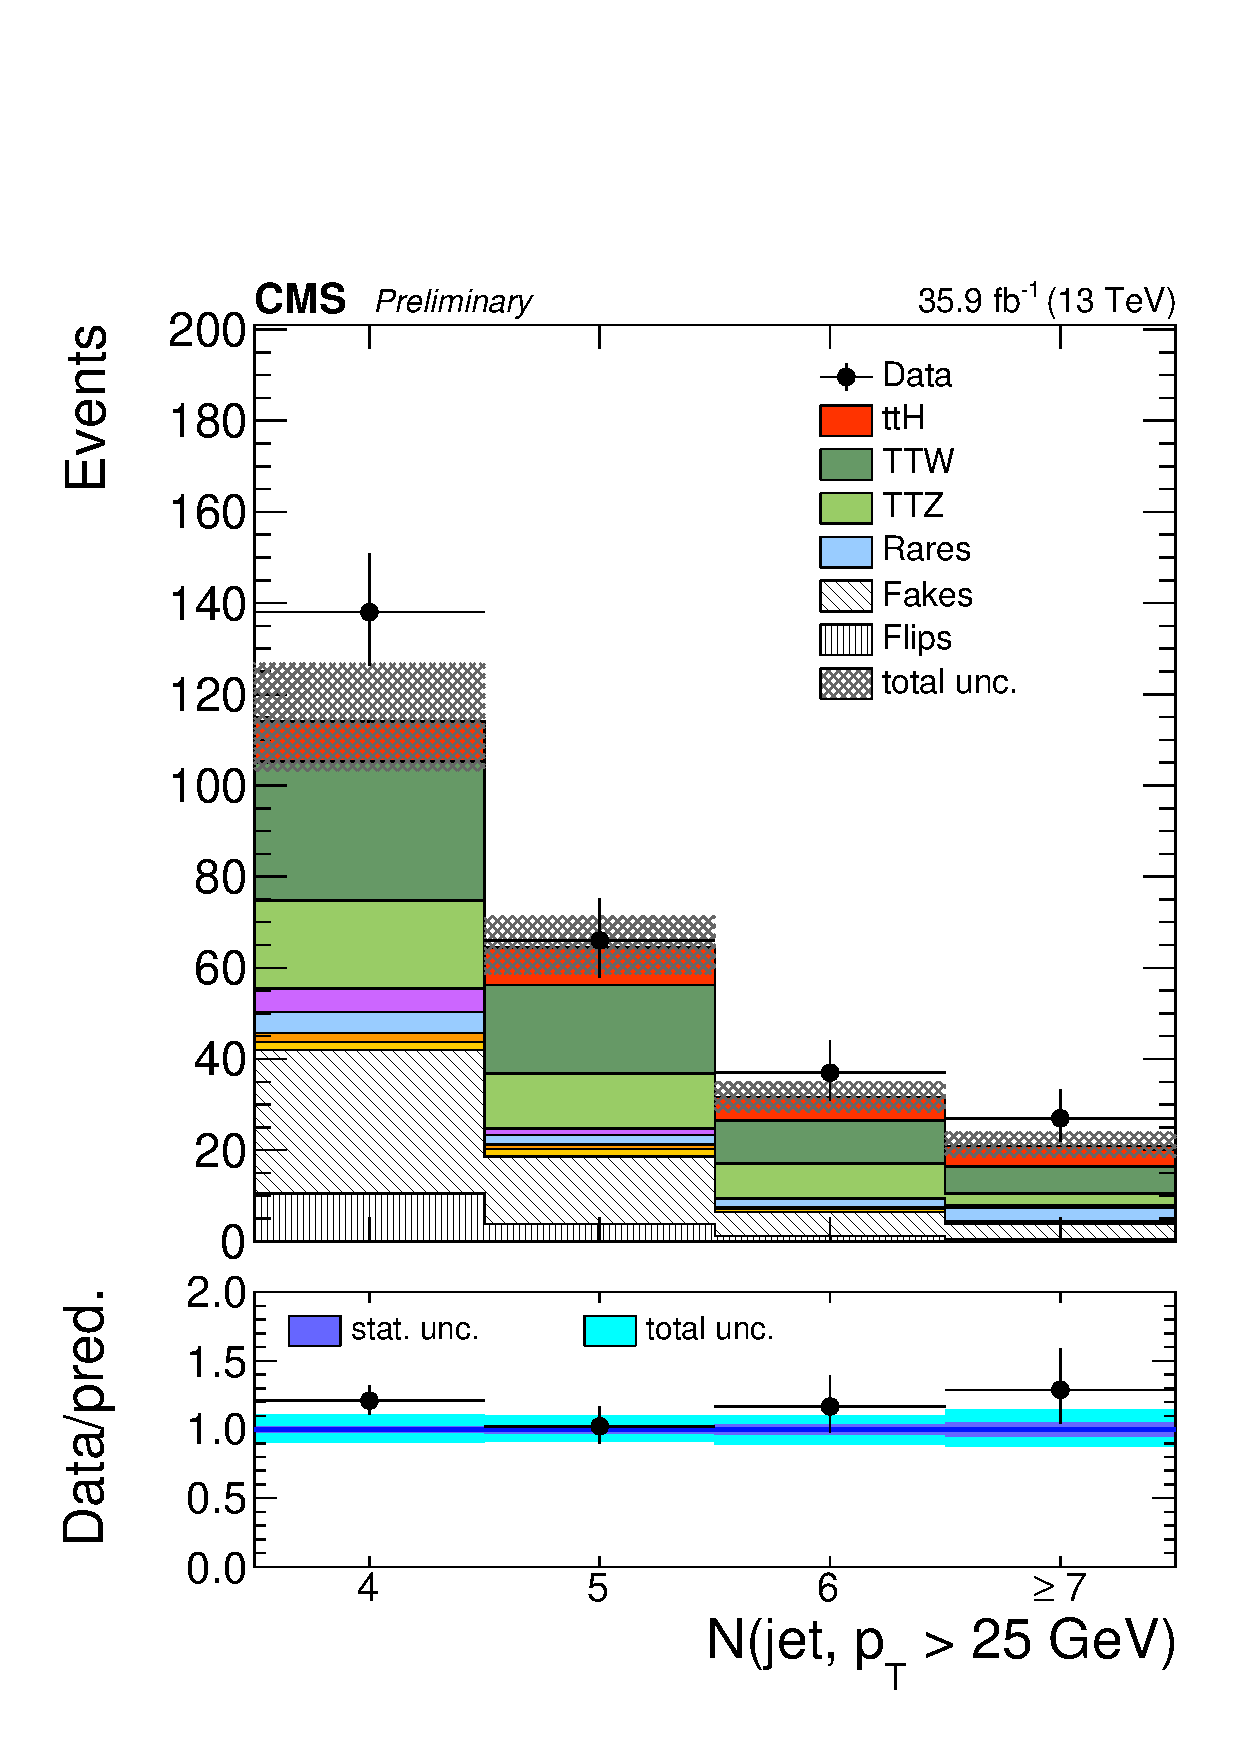
\includegraphics[width=0.32\textwidth]{plots_leptons/lep_evtsel/2lss_SR/em/2lep_nJet25_from4.pdf}
	\caption{Jet multiplicity in the 2$\ell$ ($\Pgm\Pgm$, $\Pe\Pe$, $\Pe\Pgm$) selections.}
	\label{fig:2l_nJet}
\end{figure}

\begin{figure}[htb]
	\centering 
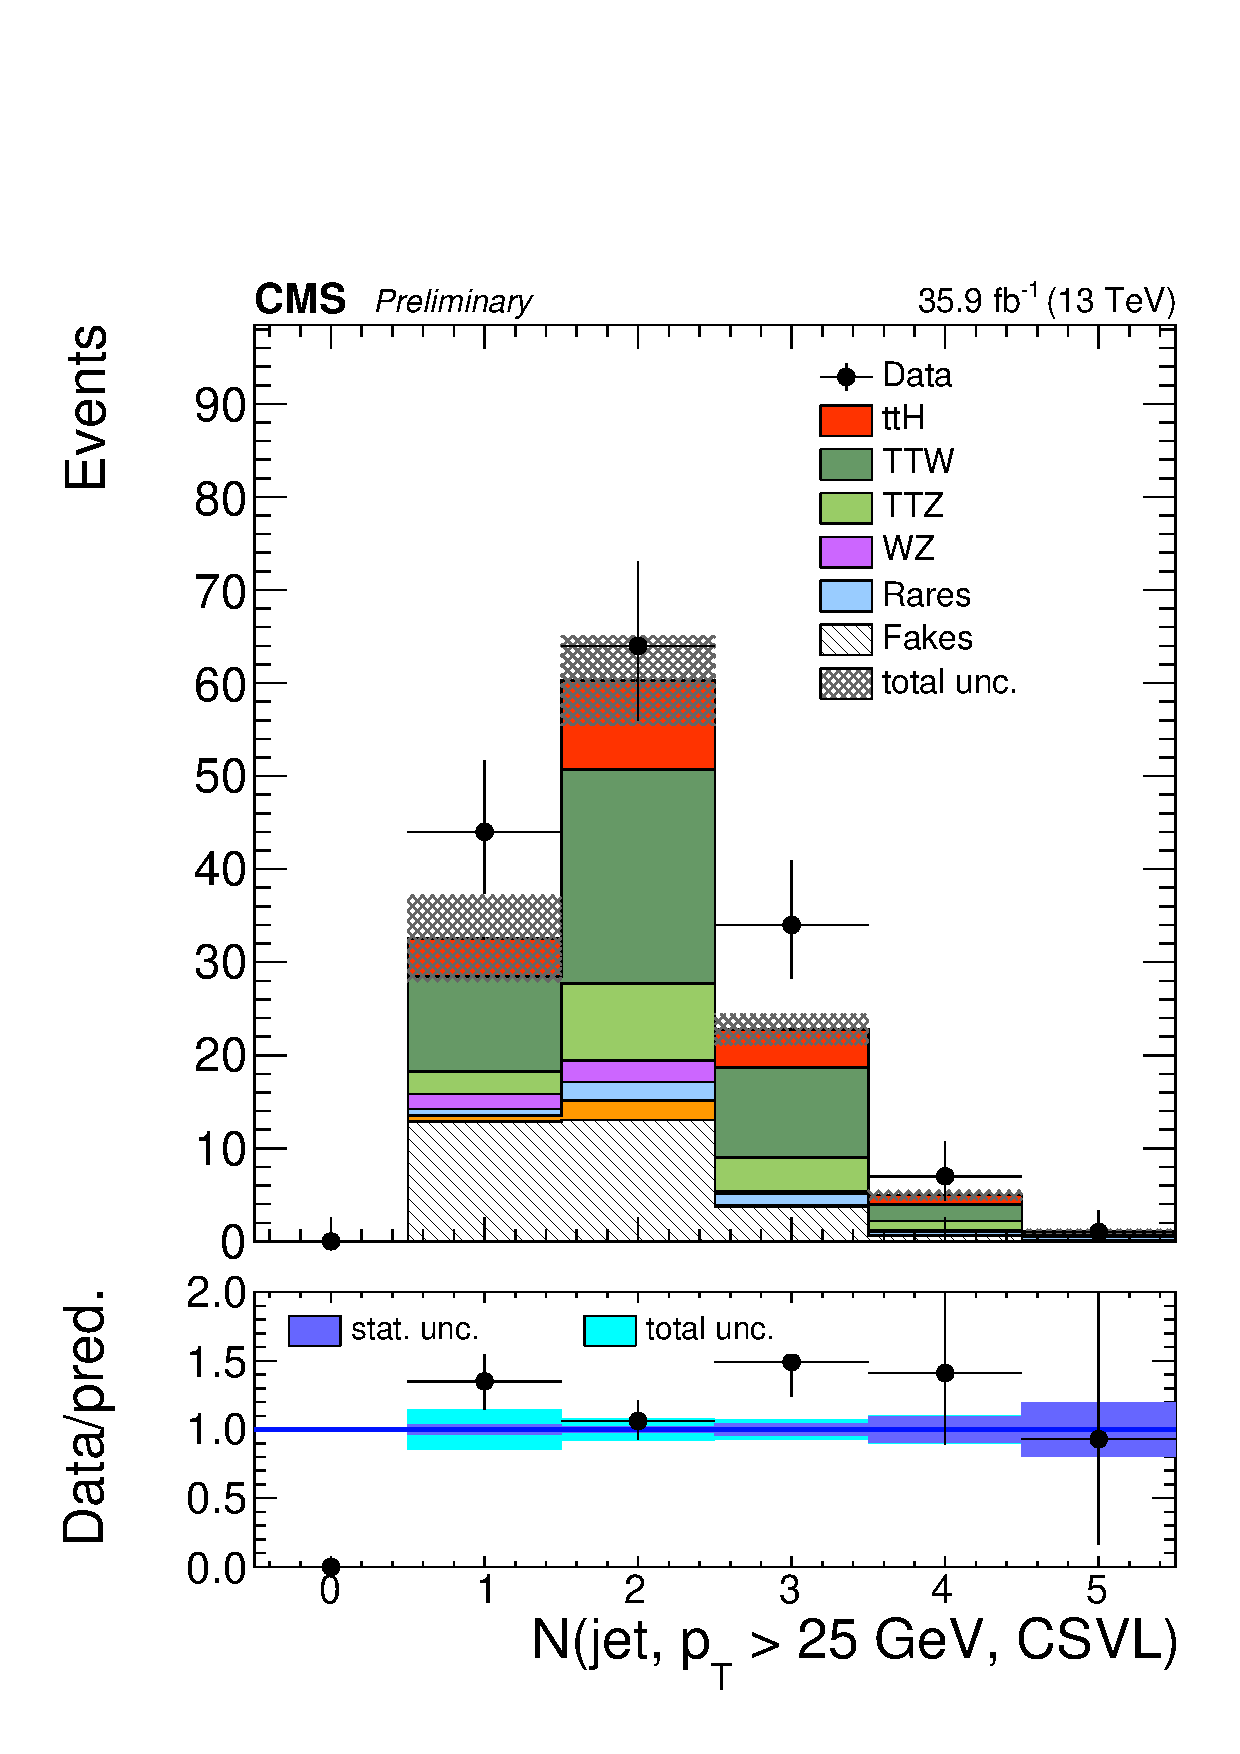
\includegraphics[width=0.32\textwidth]{plots_leptons/lep_evtsel/2lss_SR/mm/nBJetLoose25.pdf}
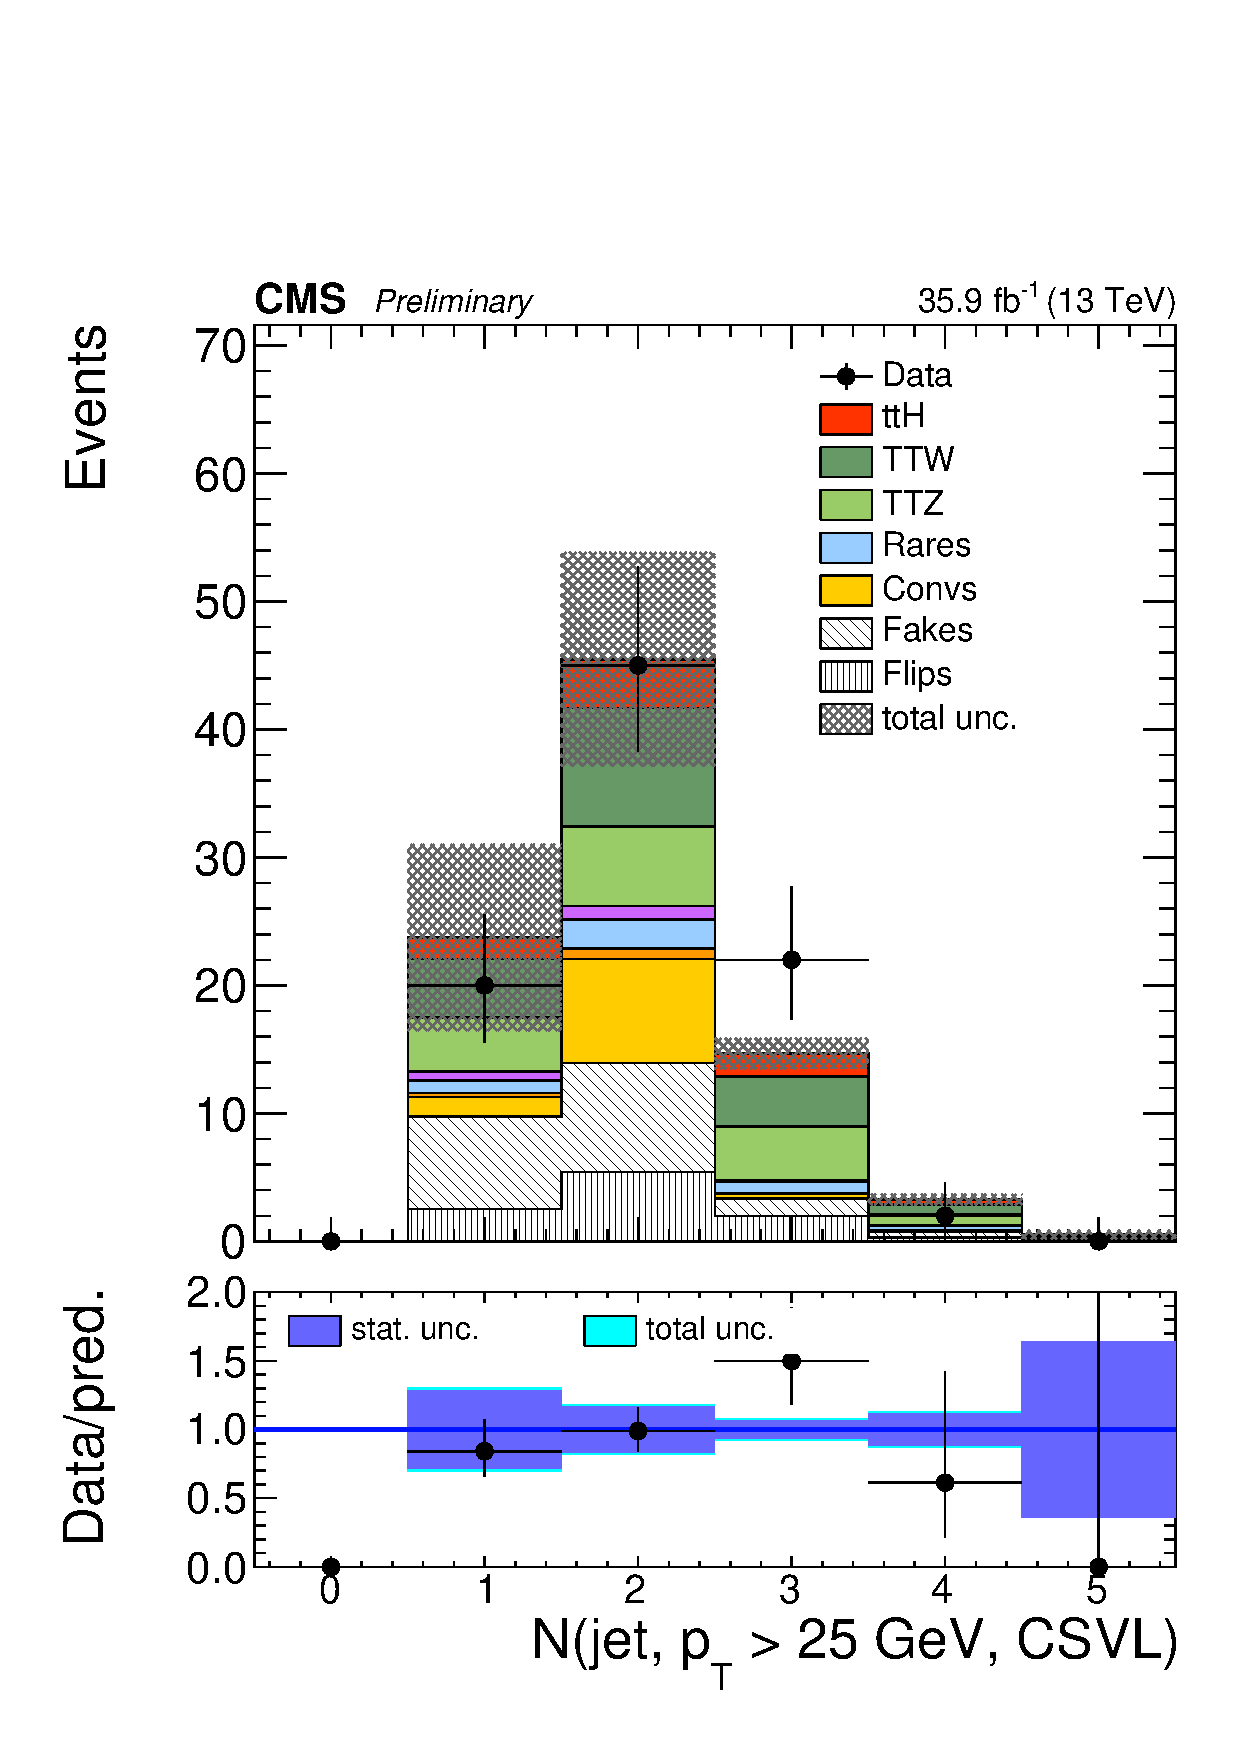
\includegraphics[width=0.32\textwidth]{plots_leptons/lep_evtsel/2lss_SR/ee/nBJetLoose25.pdf}
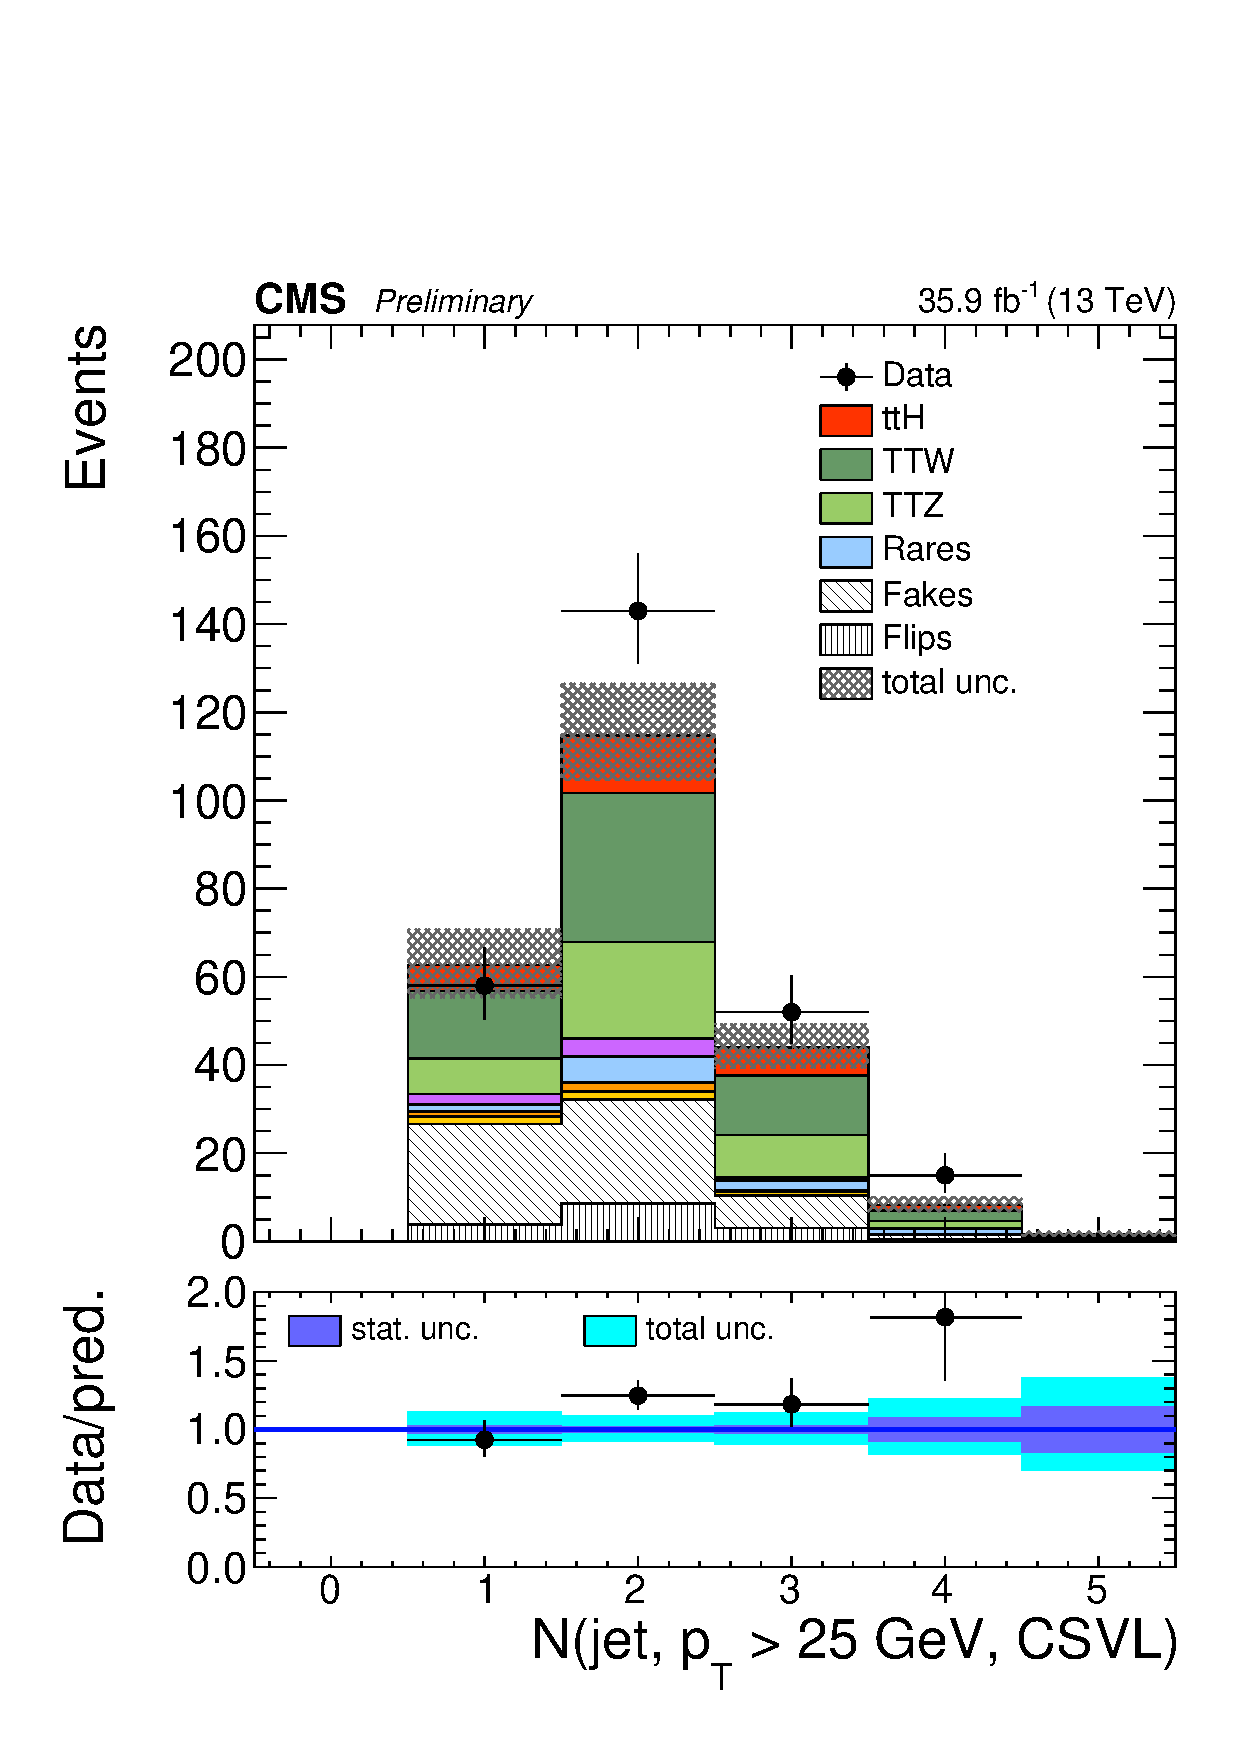
\includegraphics[width=0.32\textwidth]{plots_leptons/lep_evtsel/2lss_SR/em/nBJetLoose25.pdf}
	\caption{Multiplicity of jets passing the loose working point of the CSV tagger in the 2$\ell$ ($\Pgm\Pgm$, $\Pe\Pe$, $\Pe\Pgm$) selections.}
	\label{fig:2l_nBJetLoose}
\end{figure}

\begin{figure}[htb]
	\centering 
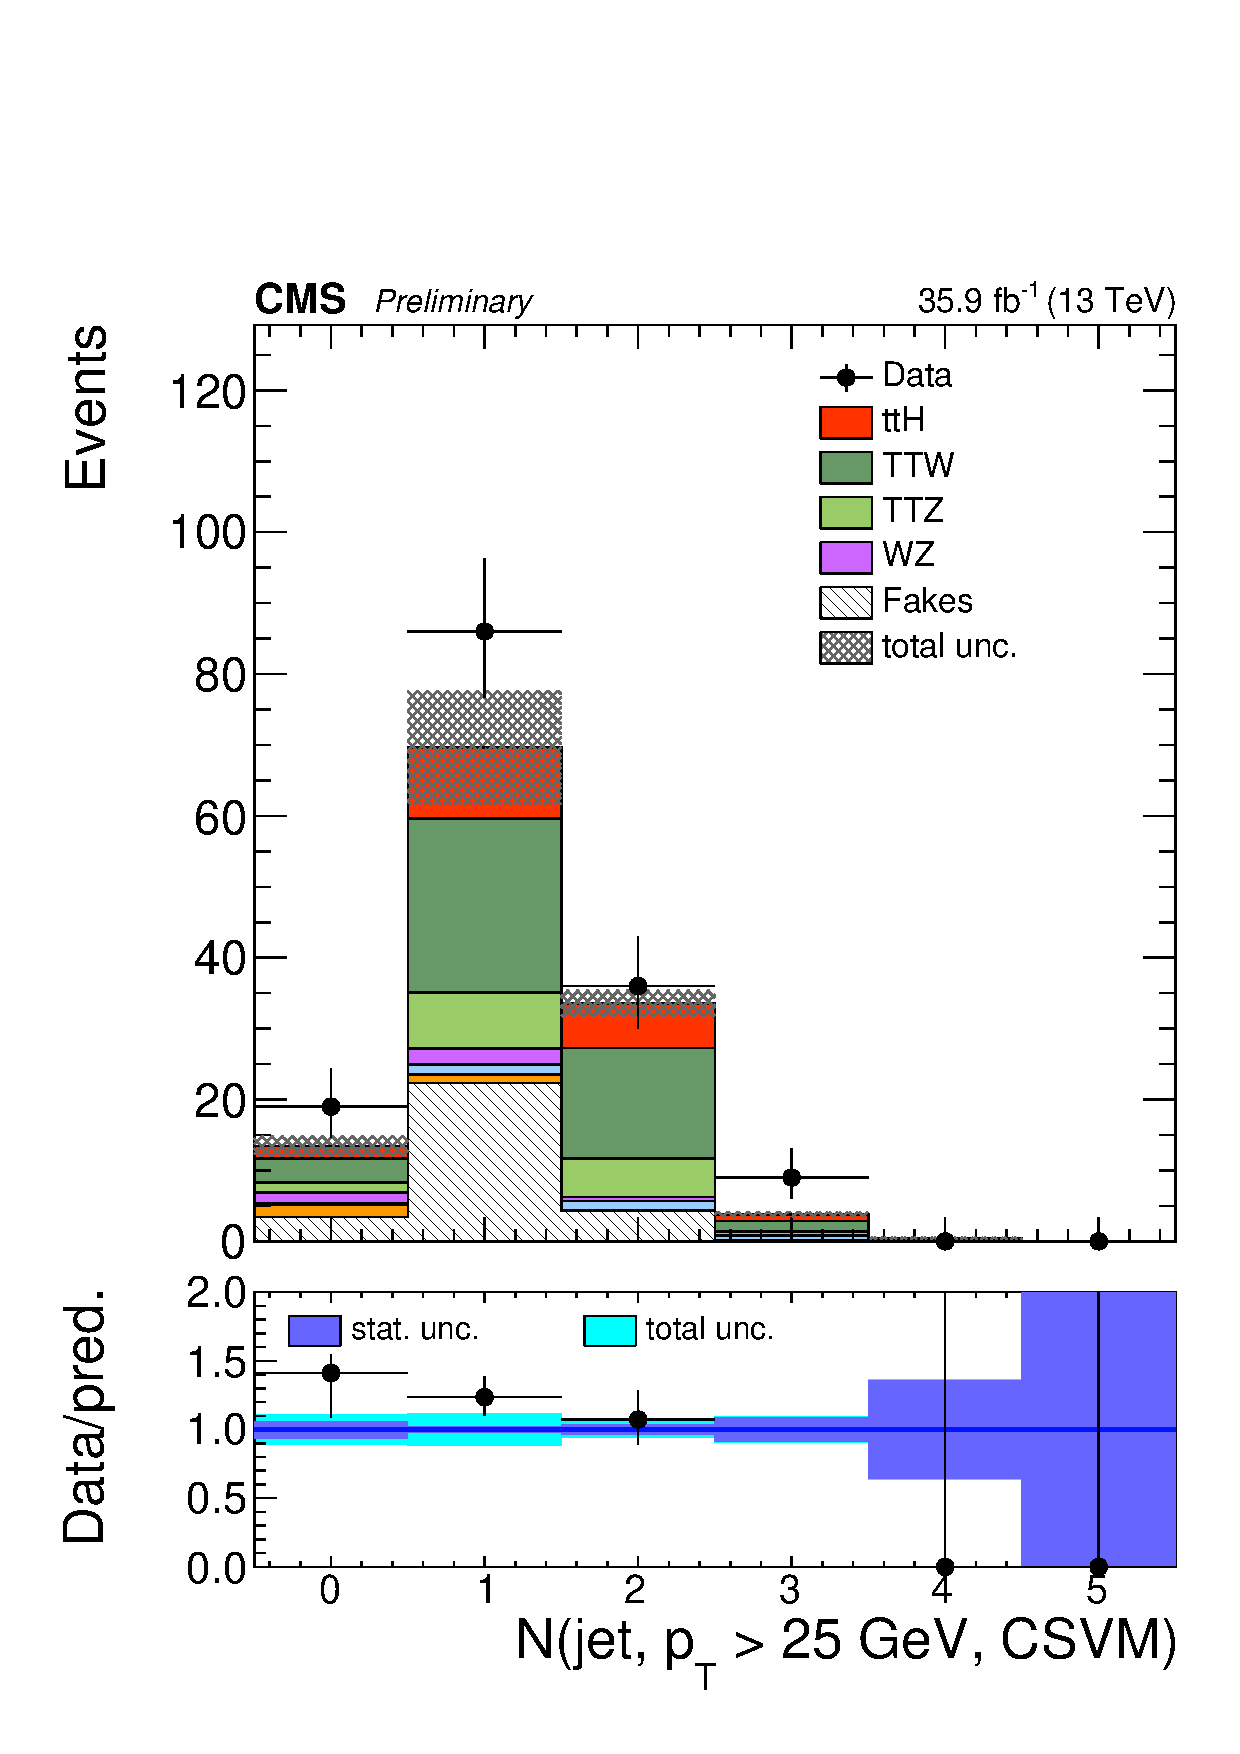
\includegraphics[width=0.32\textwidth]{plots_leptons/lep_evtsel/2lss_SR/mm/nBJetMedium25.pdf}
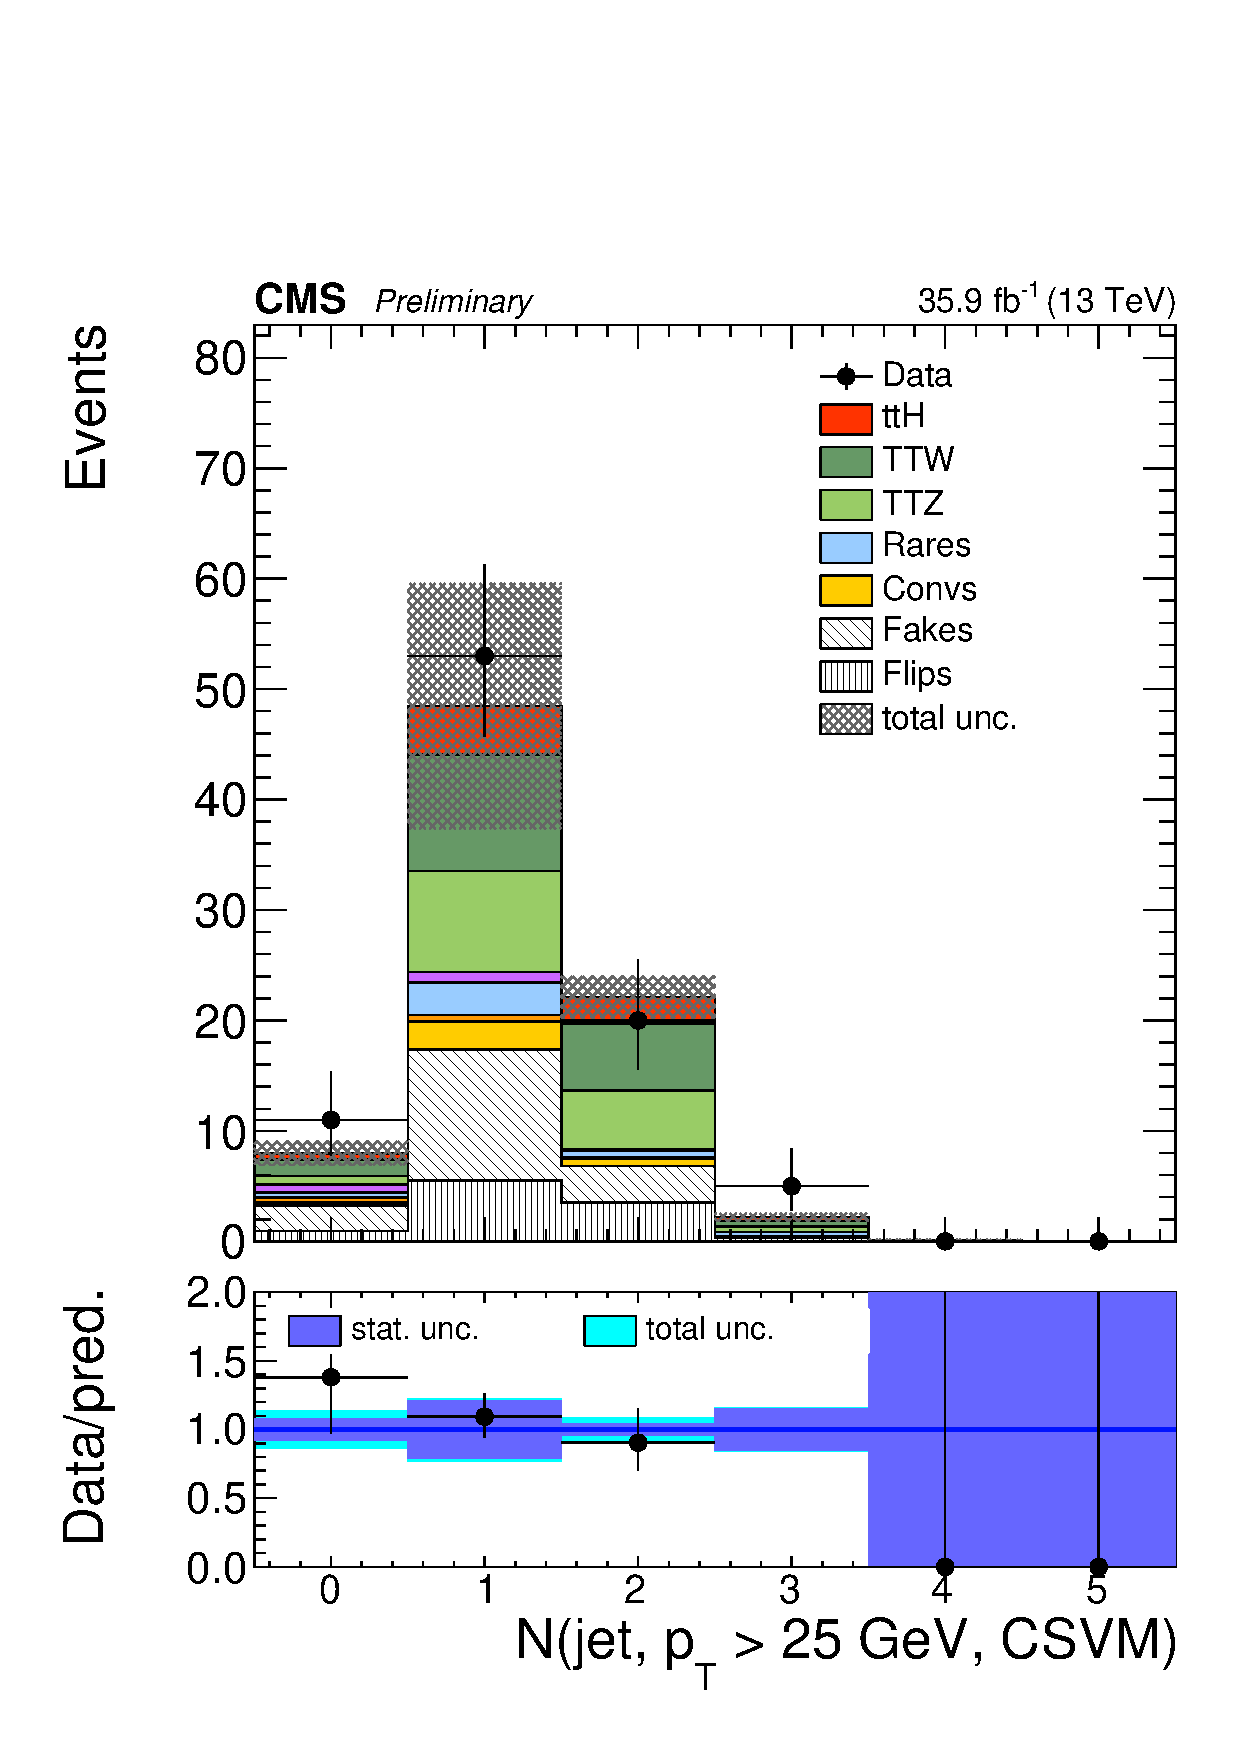
\includegraphics[width=0.32\textwidth]{plots_leptons/lep_evtsel/2lss_SR/ee/nBJetMedium25.pdf}
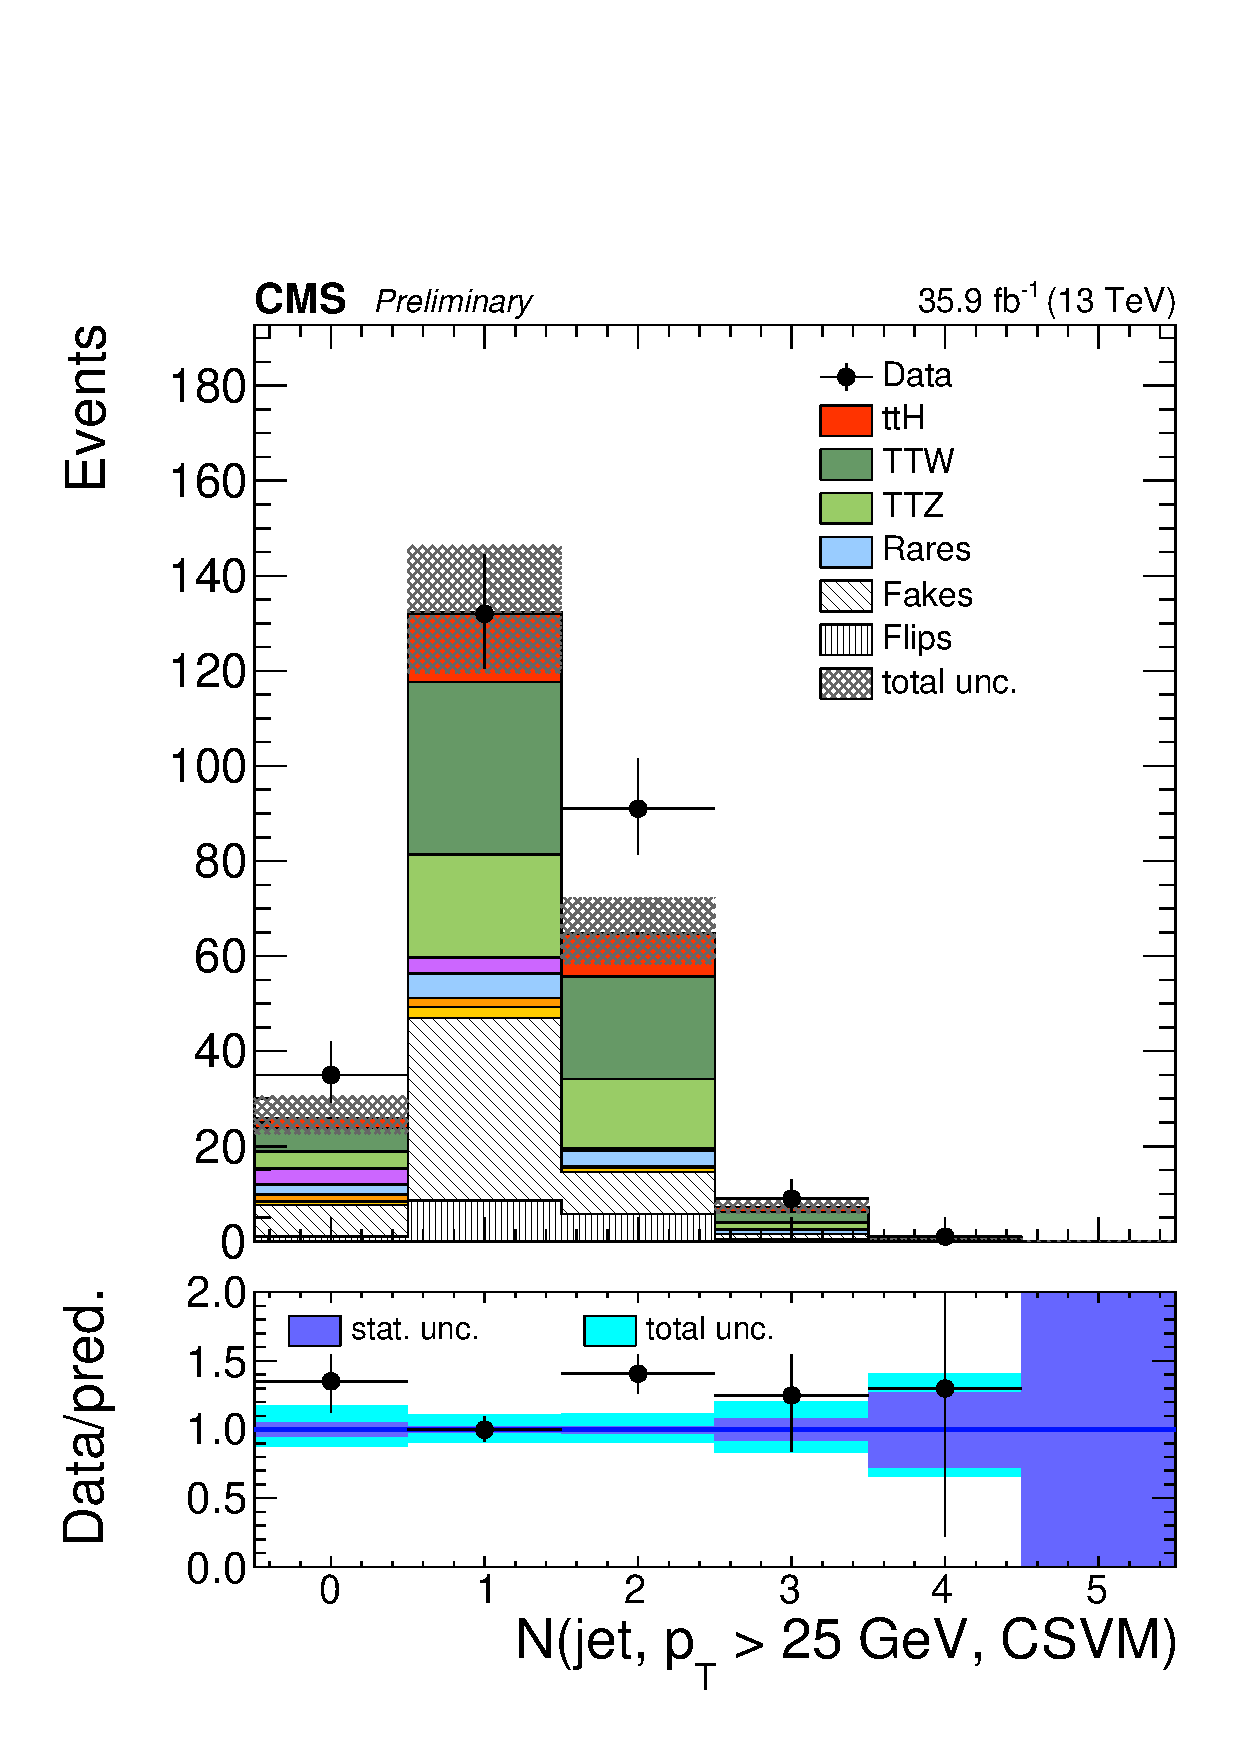
\includegraphics[width=0.32\textwidth]{plots_leptons/lep_evtsel/2lss_SR/em/nBJetMedium25.pdf}
	\caption{Multiplicity of jets passing the medium working point of the CSV tagger in the 2$\ell$ ($\Pgm\Pgm$, $\Pe\Pe$, $\Pe\Pgm$) selections.}
	\label{fig:2l_nBJetMedium}
\end{figure}


\begin{figure}[htb]
	\centering 
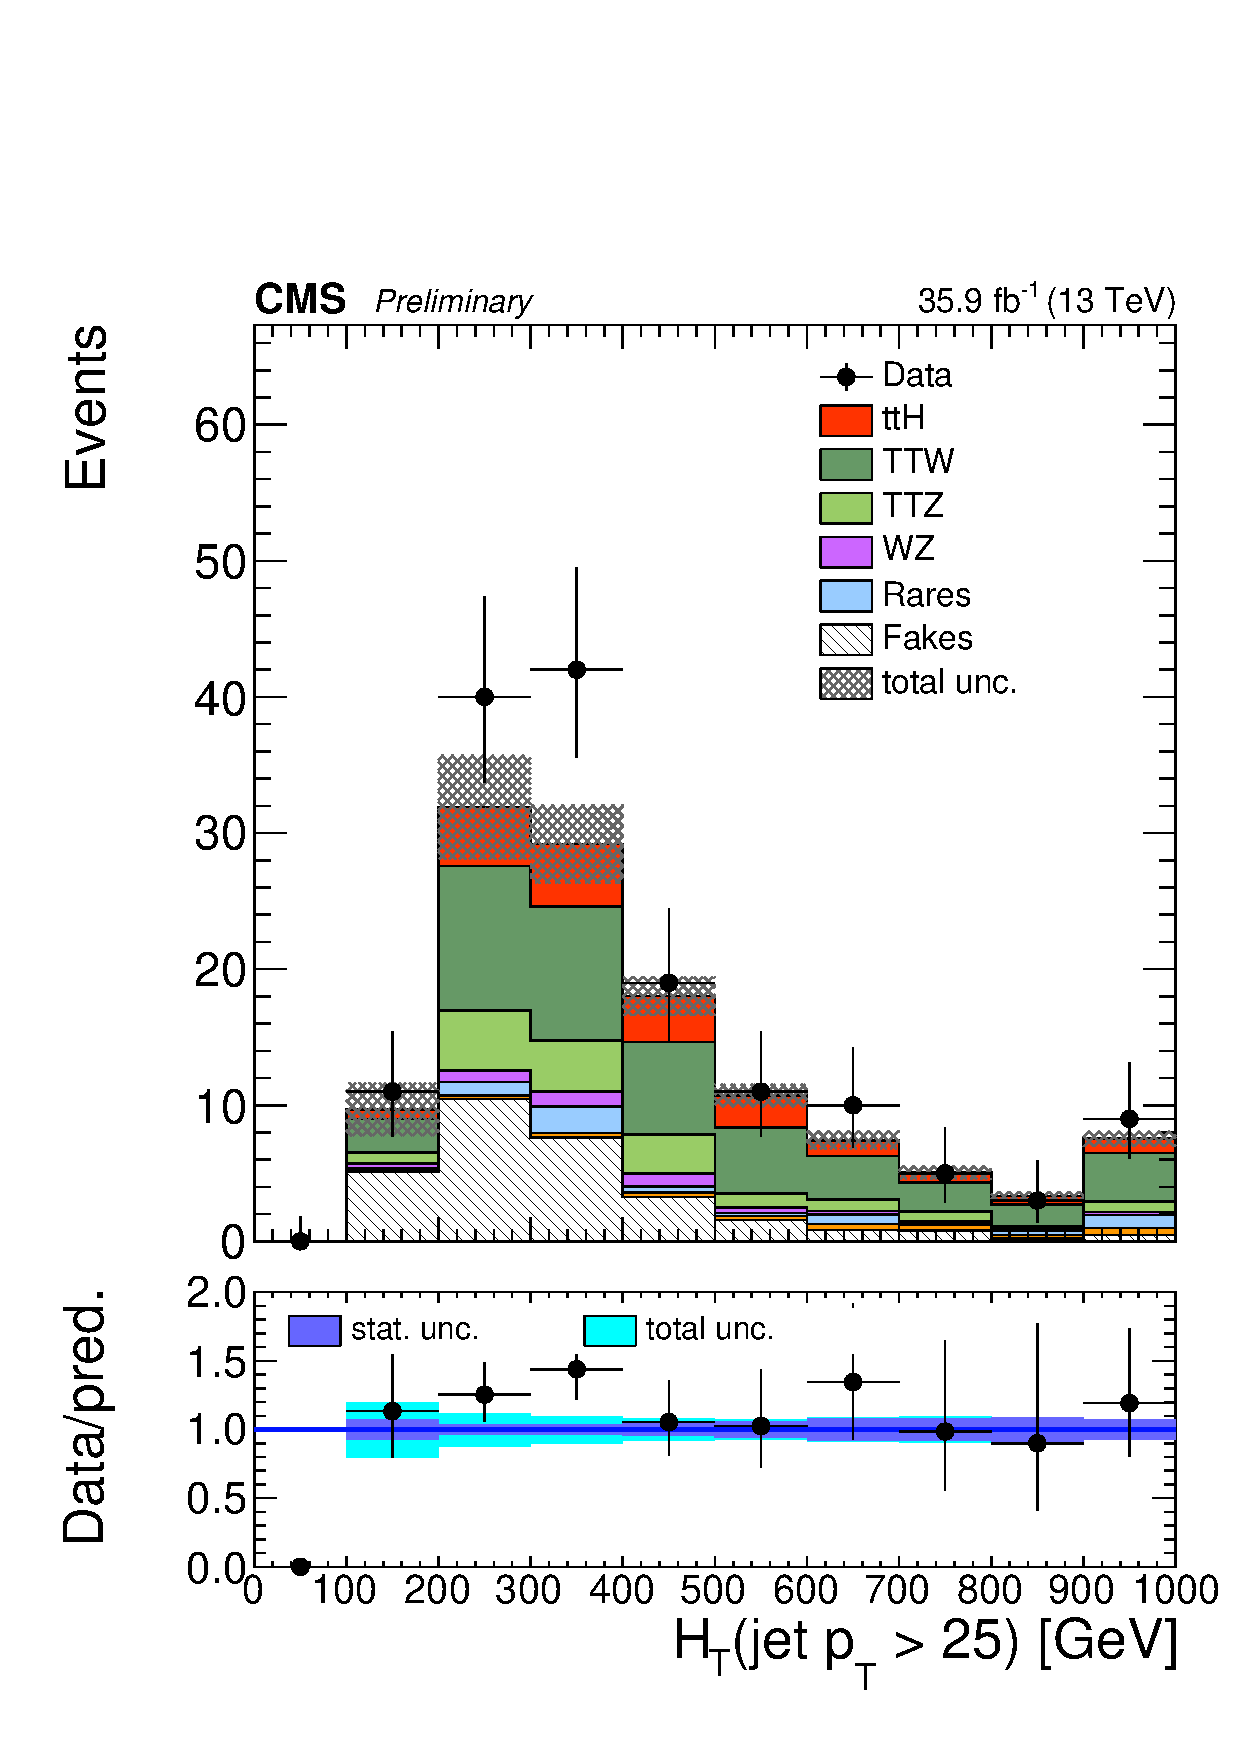
\includegraphics[width=0.32\textwidth]{plots_leptons/lep_evtsel/2lss_SR/mm/htJet25j.pdf}
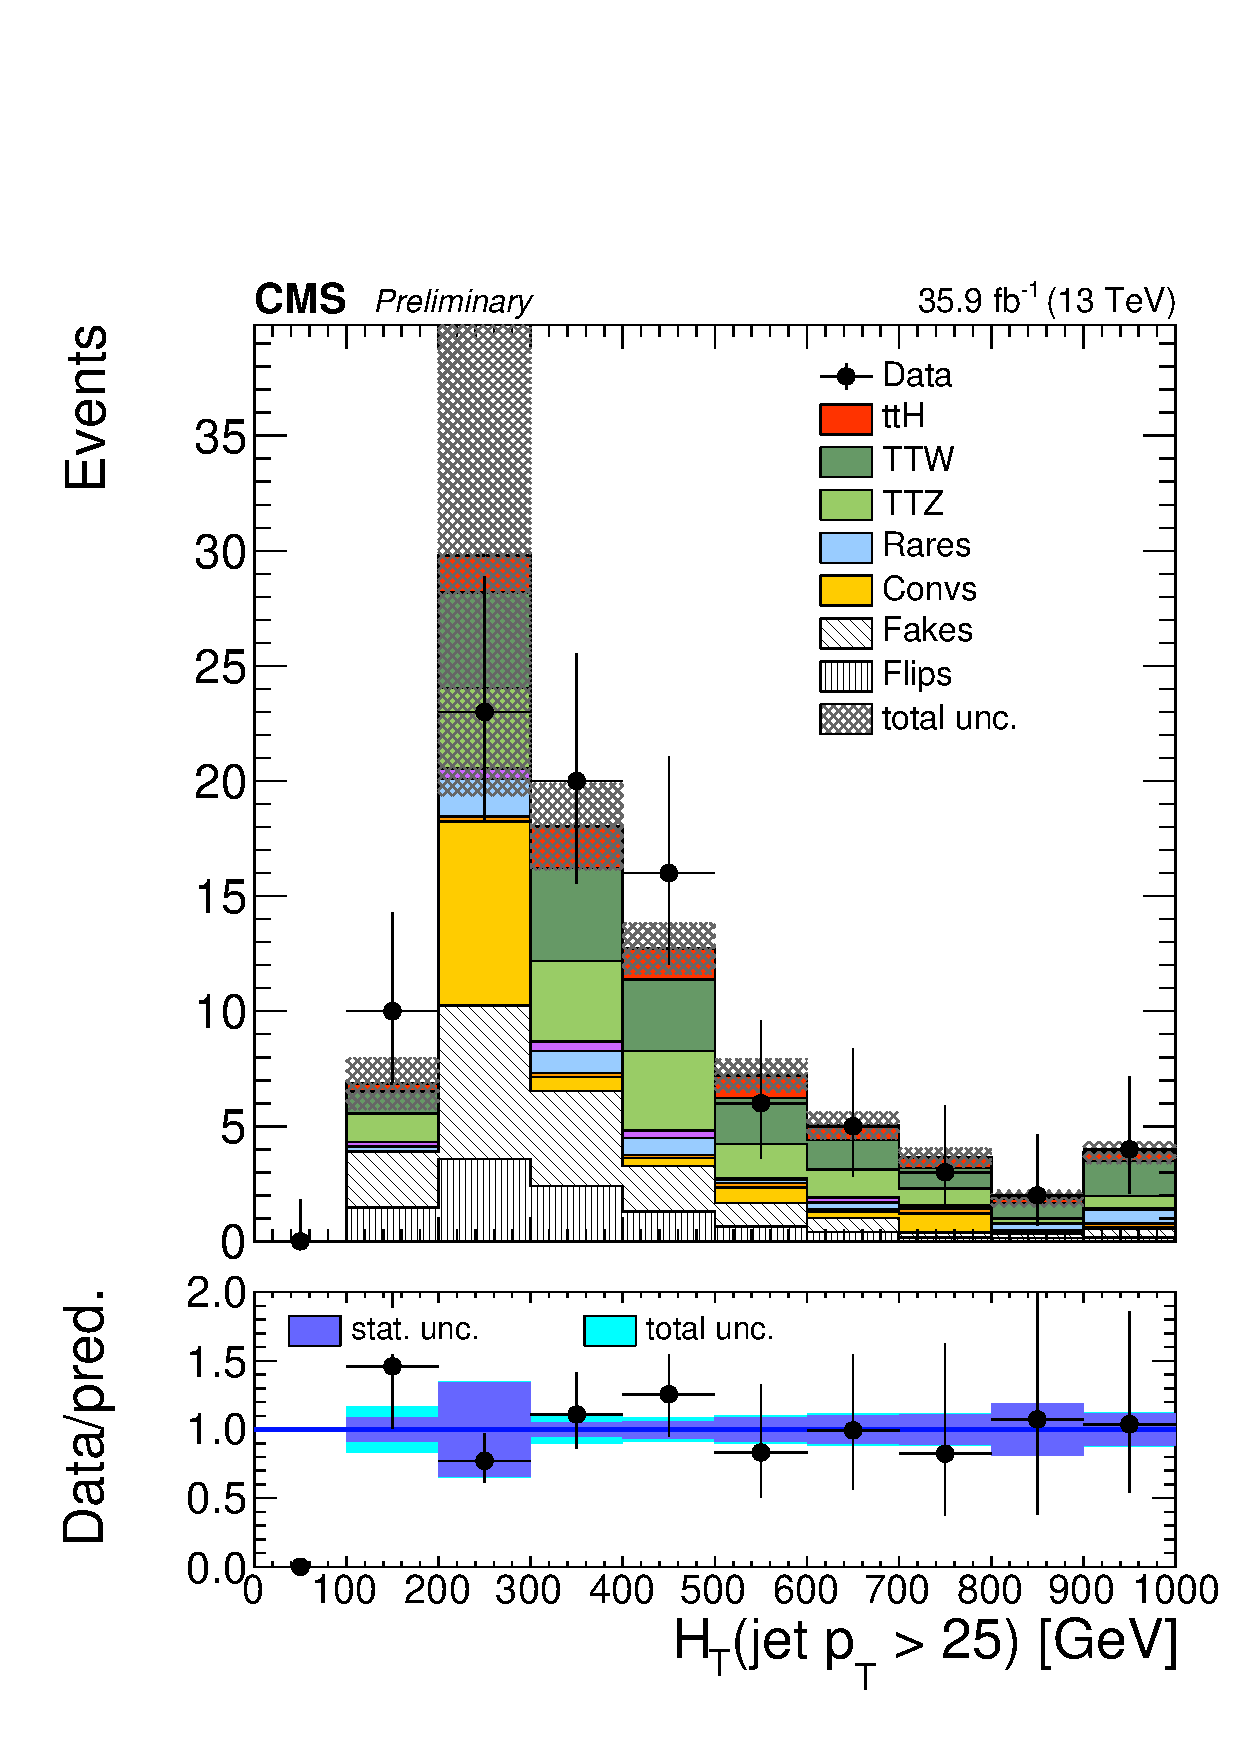
\includegraphics[width=0.32\textwidth]{plots_leptons/lep_evtsel/2lss_SR/ee/htJet25j.pdf}
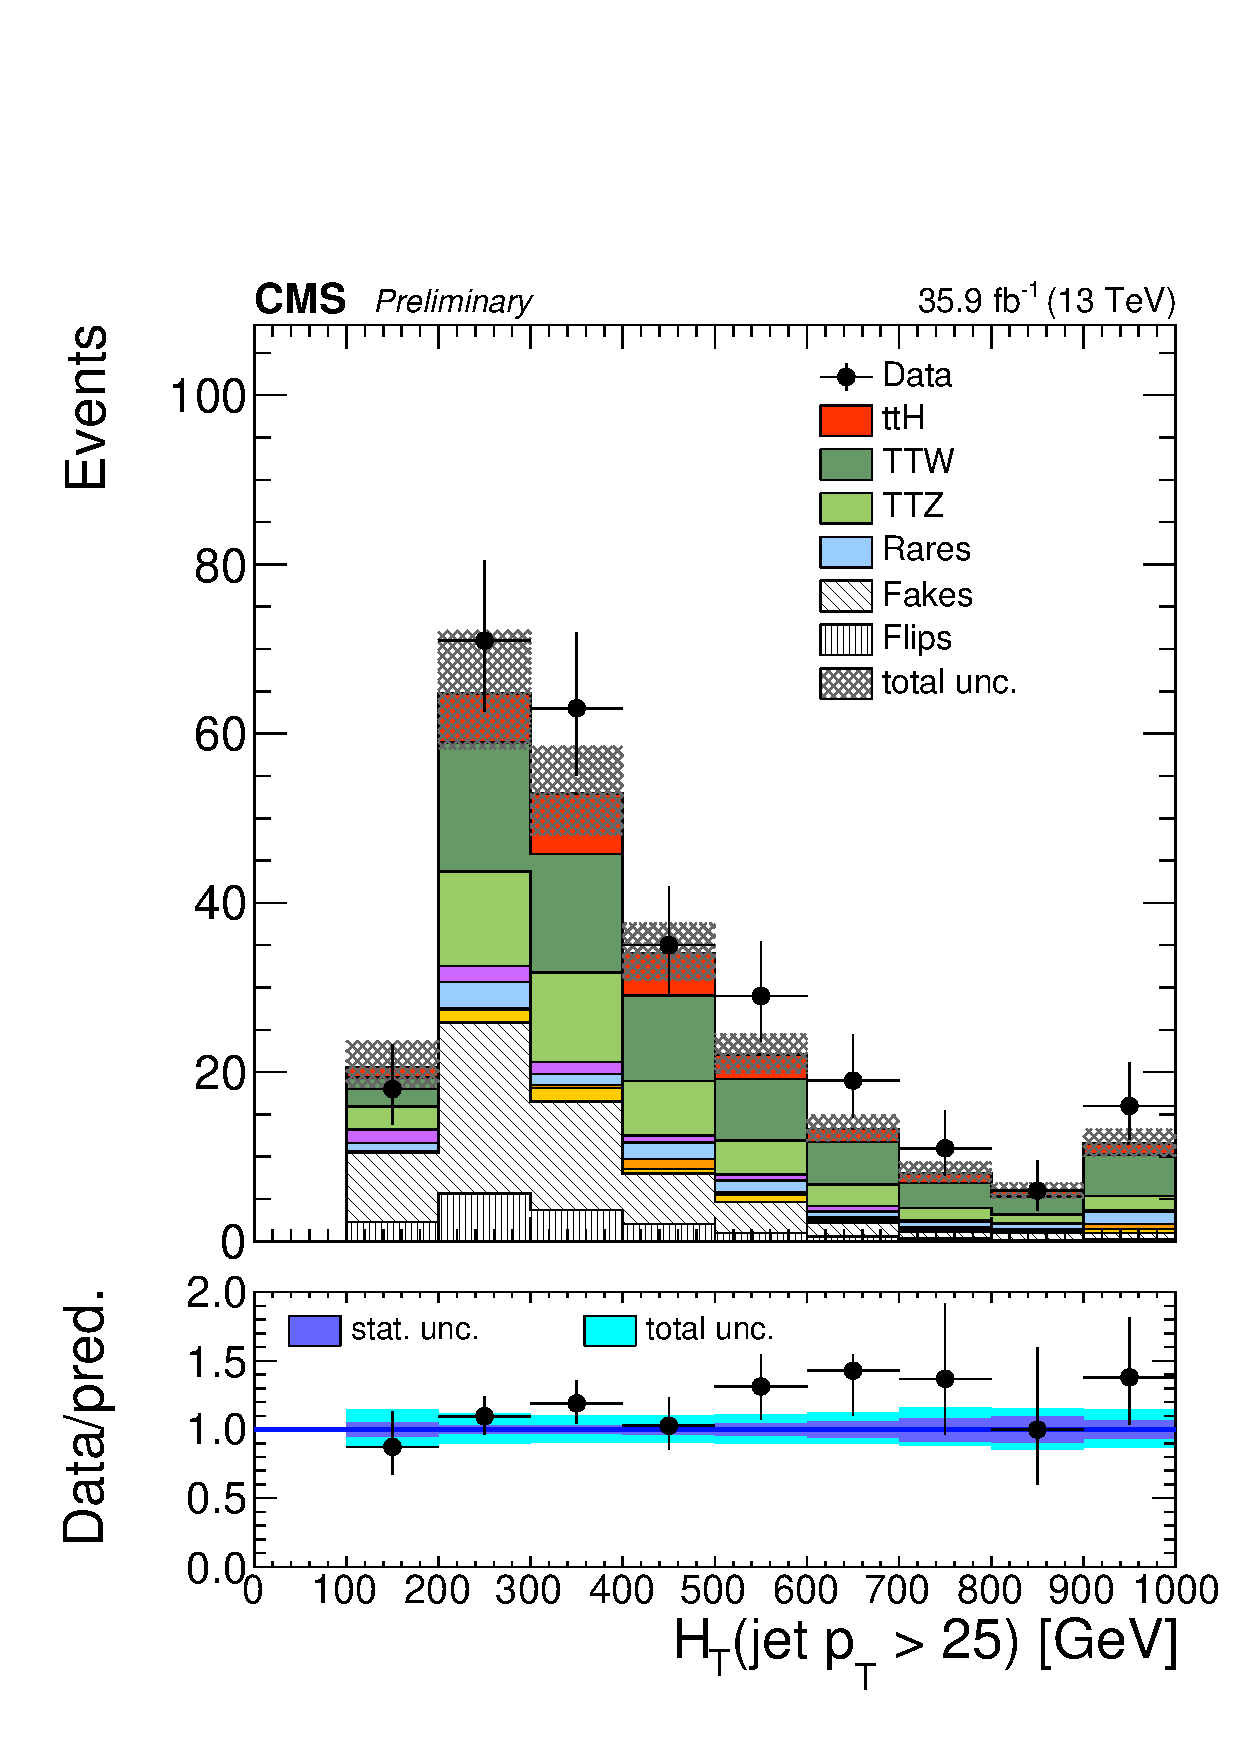
\includegraphics[width=0.32\textwidth]{plots_leptons/lep_evtsel/2lss_SR/em/htJet25j.pdf}
	\caption{$H_T$ spectra in the 2$\ell$ ($\Pgm\Pgm$, $\Pe\Pe$, $\Pe\Pgm$) selections.}
	\label{fig:2l_ht}
\end{figure}
\begin{figure}[htb]
	\centering 
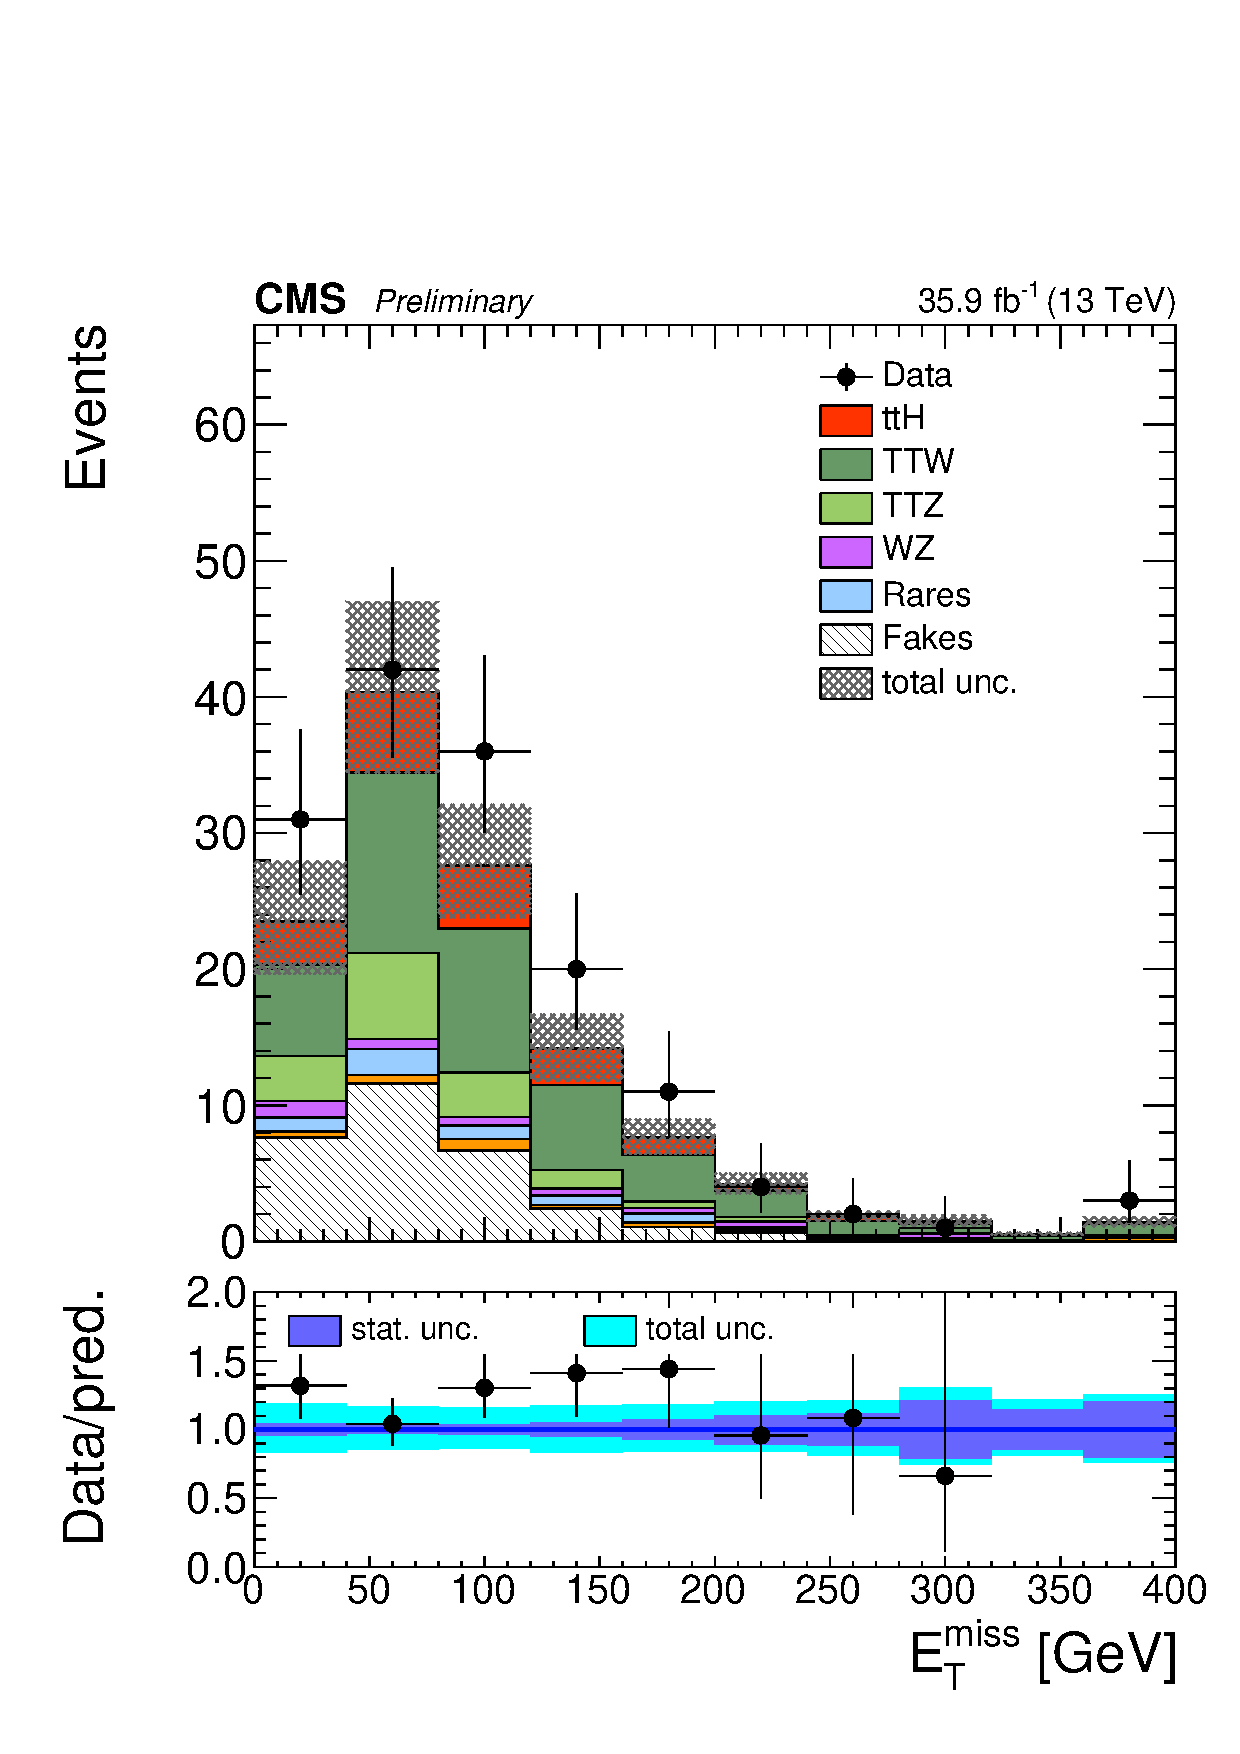
\includegraphics[width=0.32\textwidth]{plots_leptons/lep_evtsel/2lss_SR/mm/kinMVA_input_met.pdf}
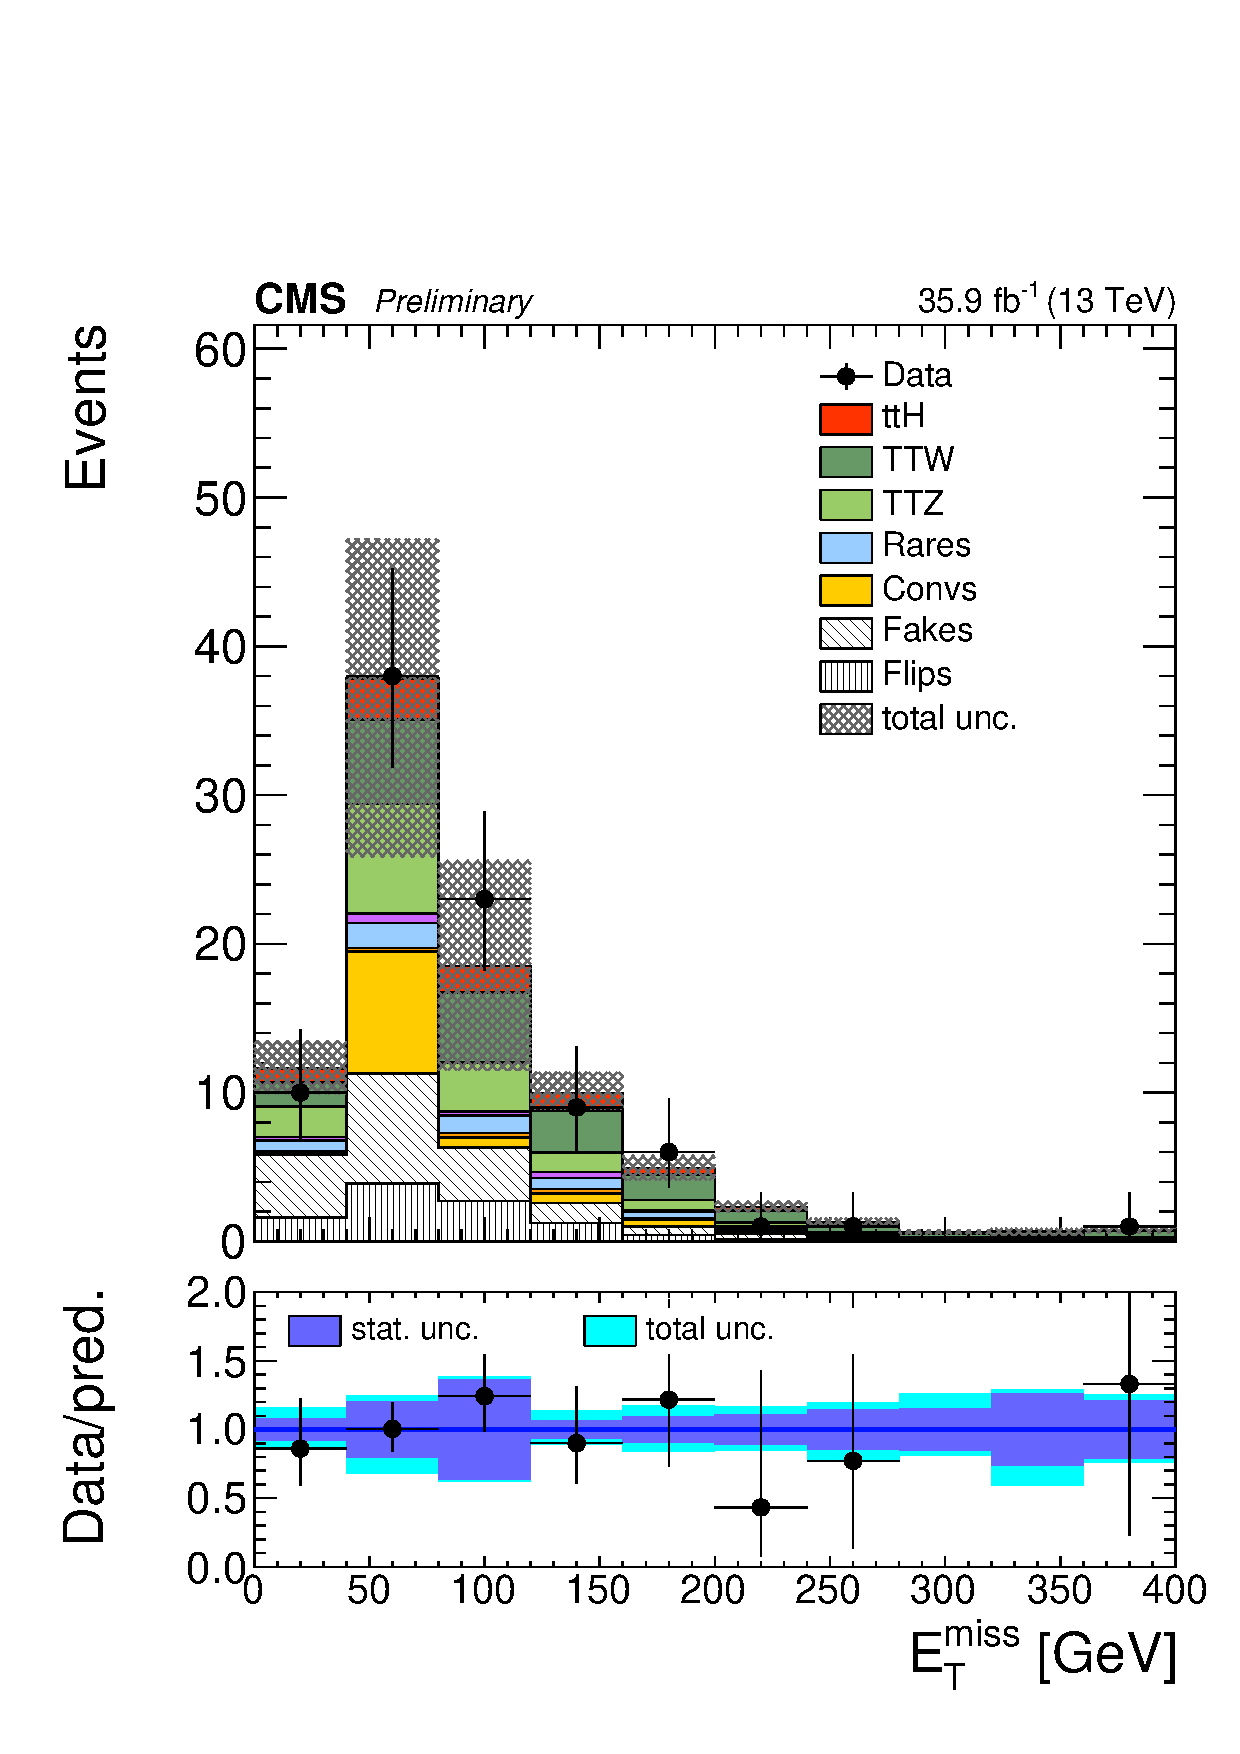
\includegraphics[width=0.32\textwidth]{plots_leptons/lep_evtsel/2lss_SR/ee/kinMVA_input_met.pdf}
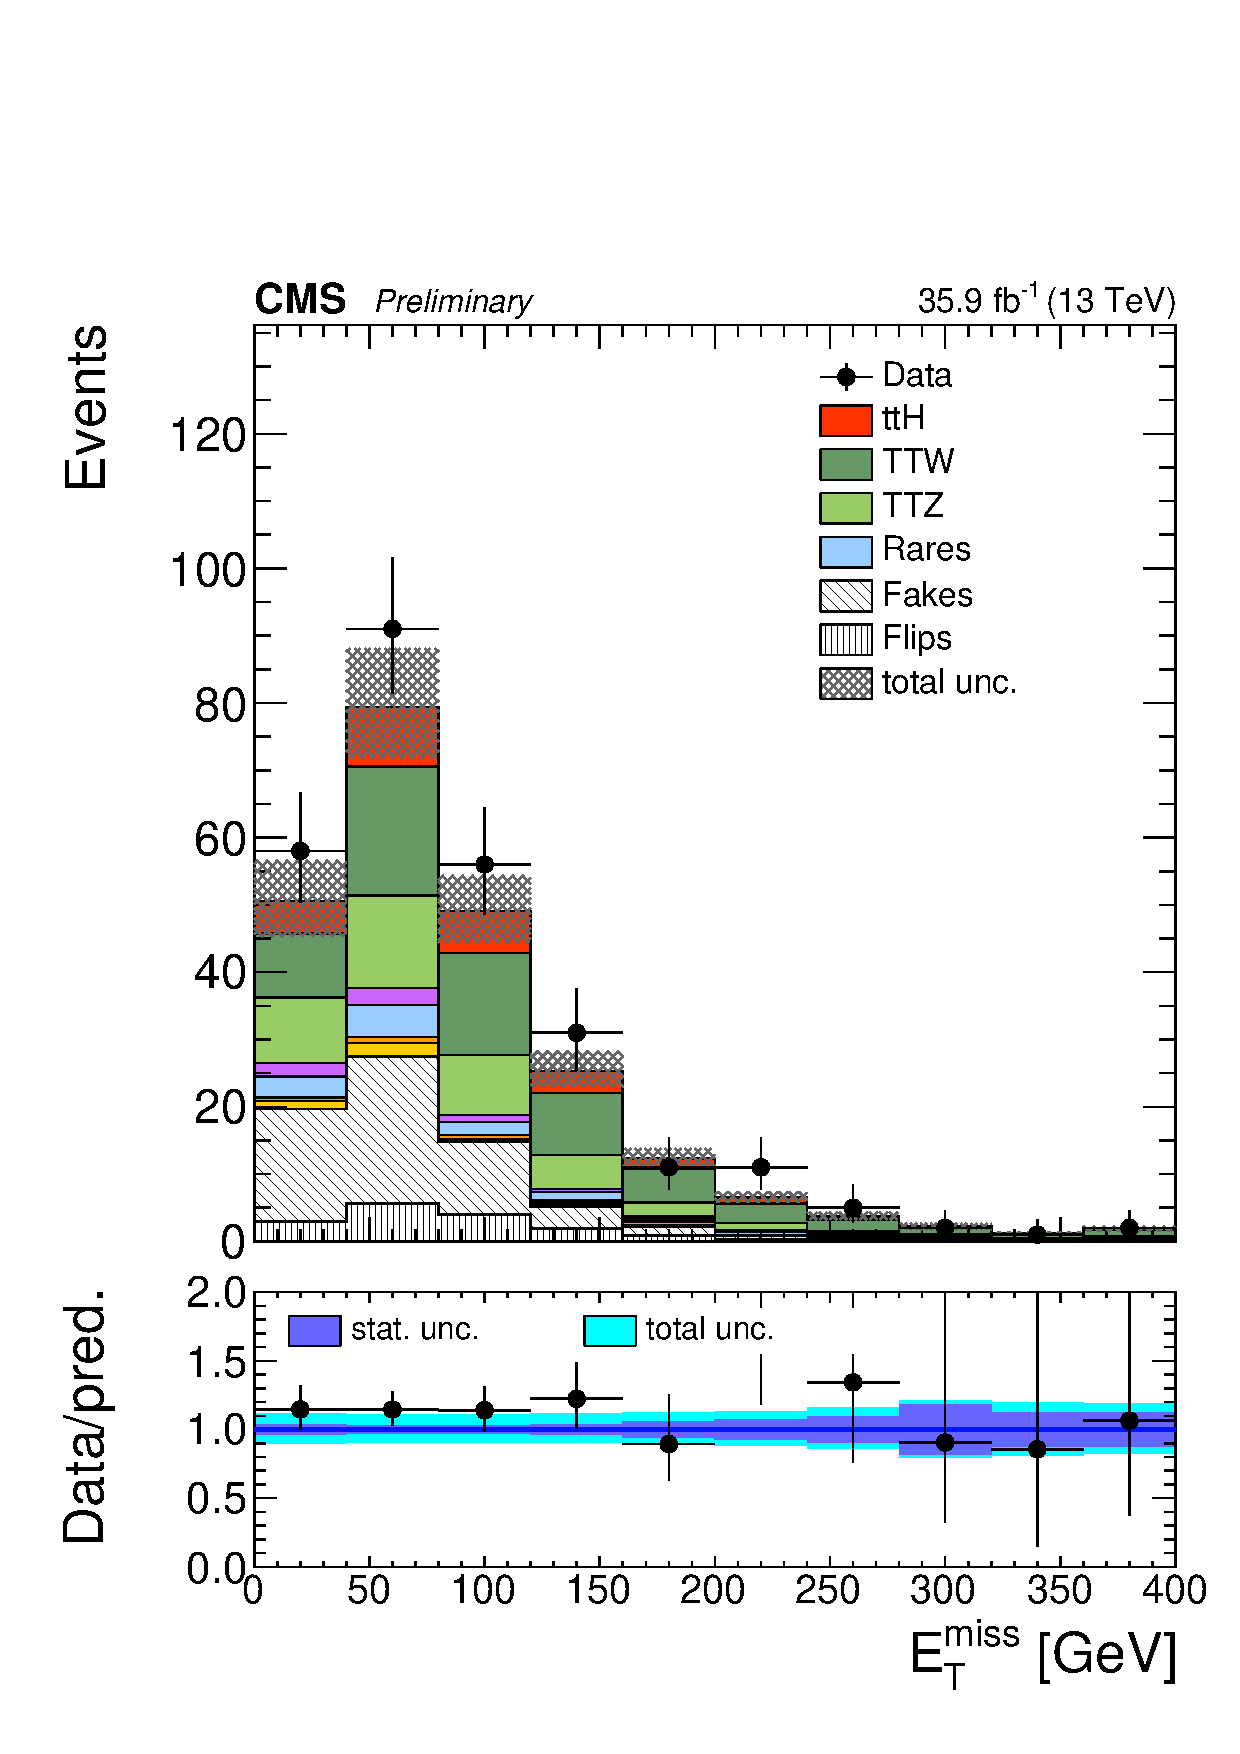
\includegraphics[width=0.32\textwidth]{plots_leptons/lep_evtsel/2lss_SR/em/kinMVA_input_met.pdf}
	\caption{$E_\mathrm{T}^\mathrm{miss}$ spectra in the 2$\ell$ ($\Pgm\Pgm$, $\Pe\Pe$, $\Pe\Pgm$) selections.}
	\label{fig:2l_met}
\end{figure}
\begin{figure}[htb]
	\centering 
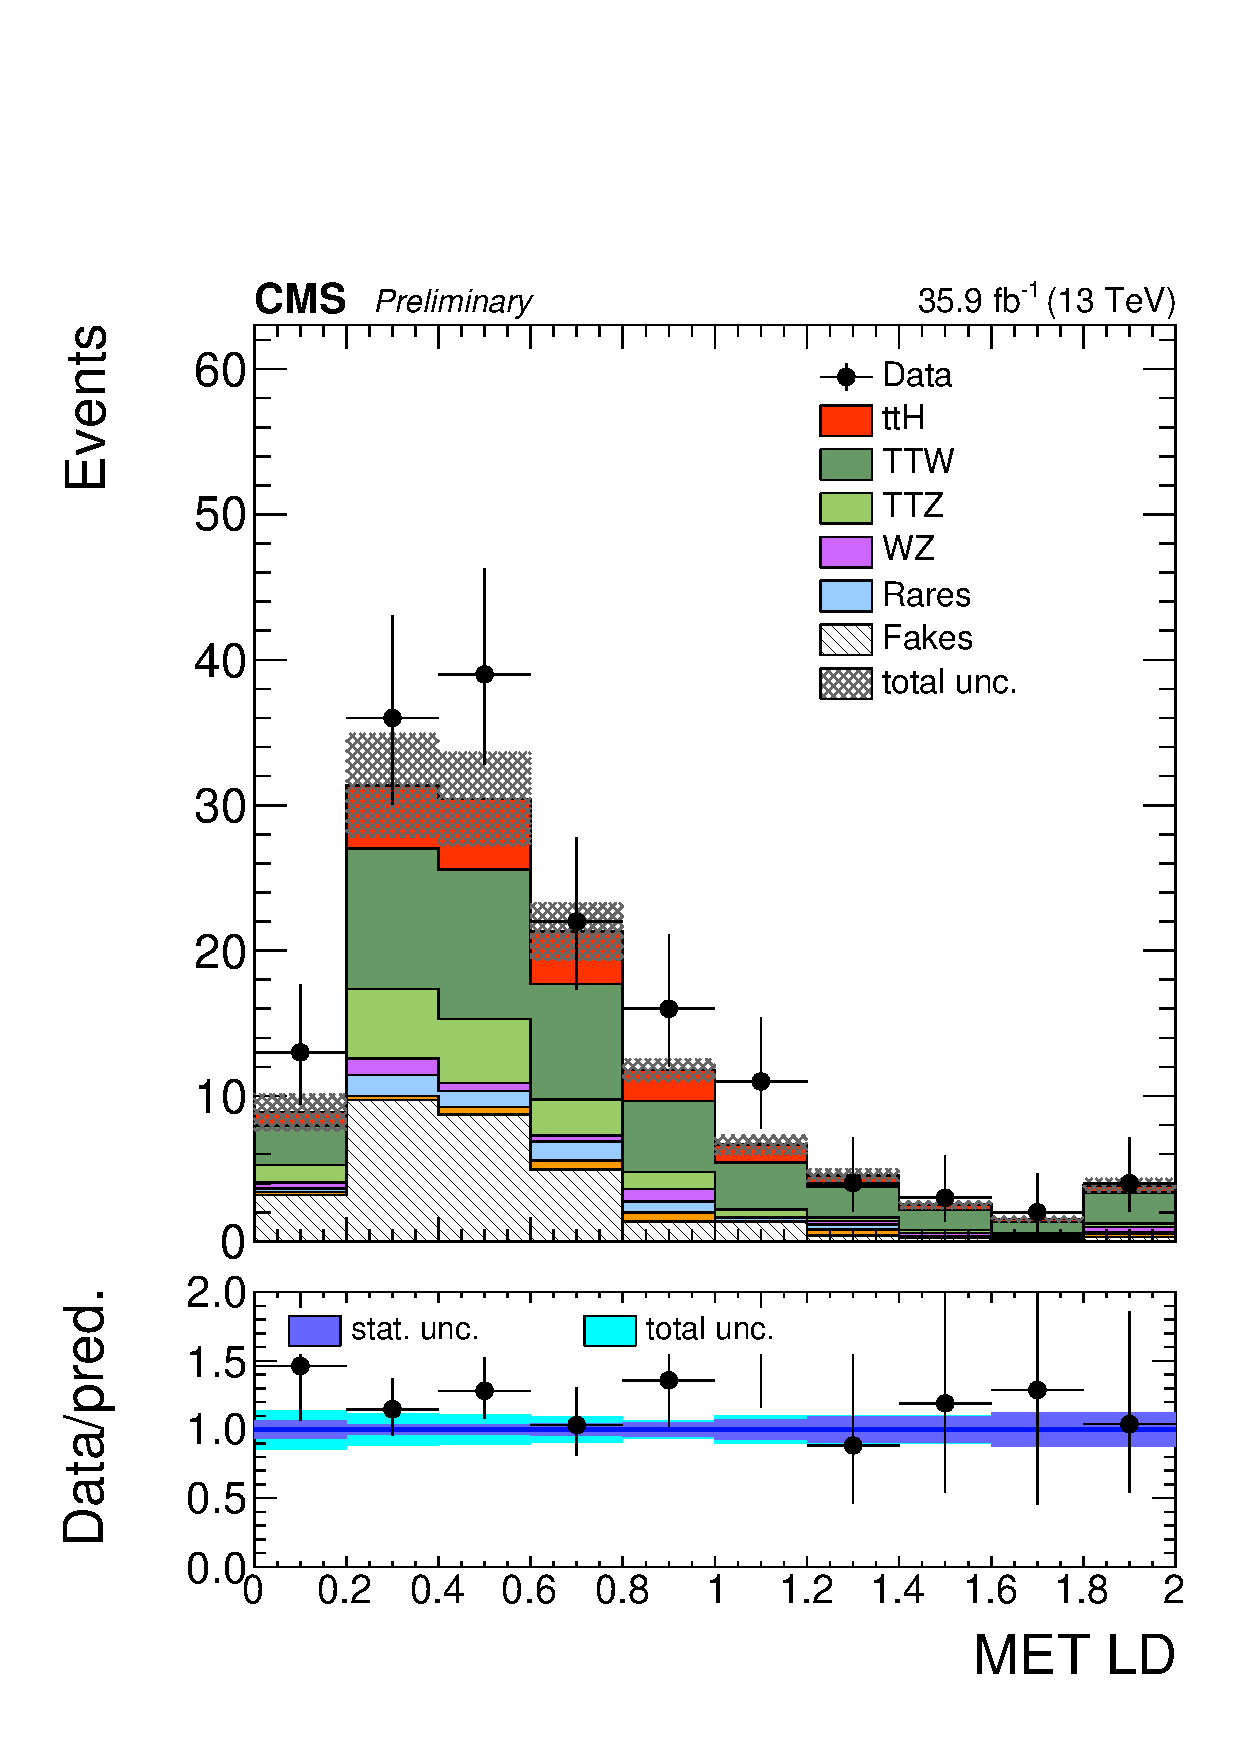
\includegraphics[width=0.32\textwidth]{plots_leptons/lep_evtsel/2lss_SR/mm/metLD.pdf}
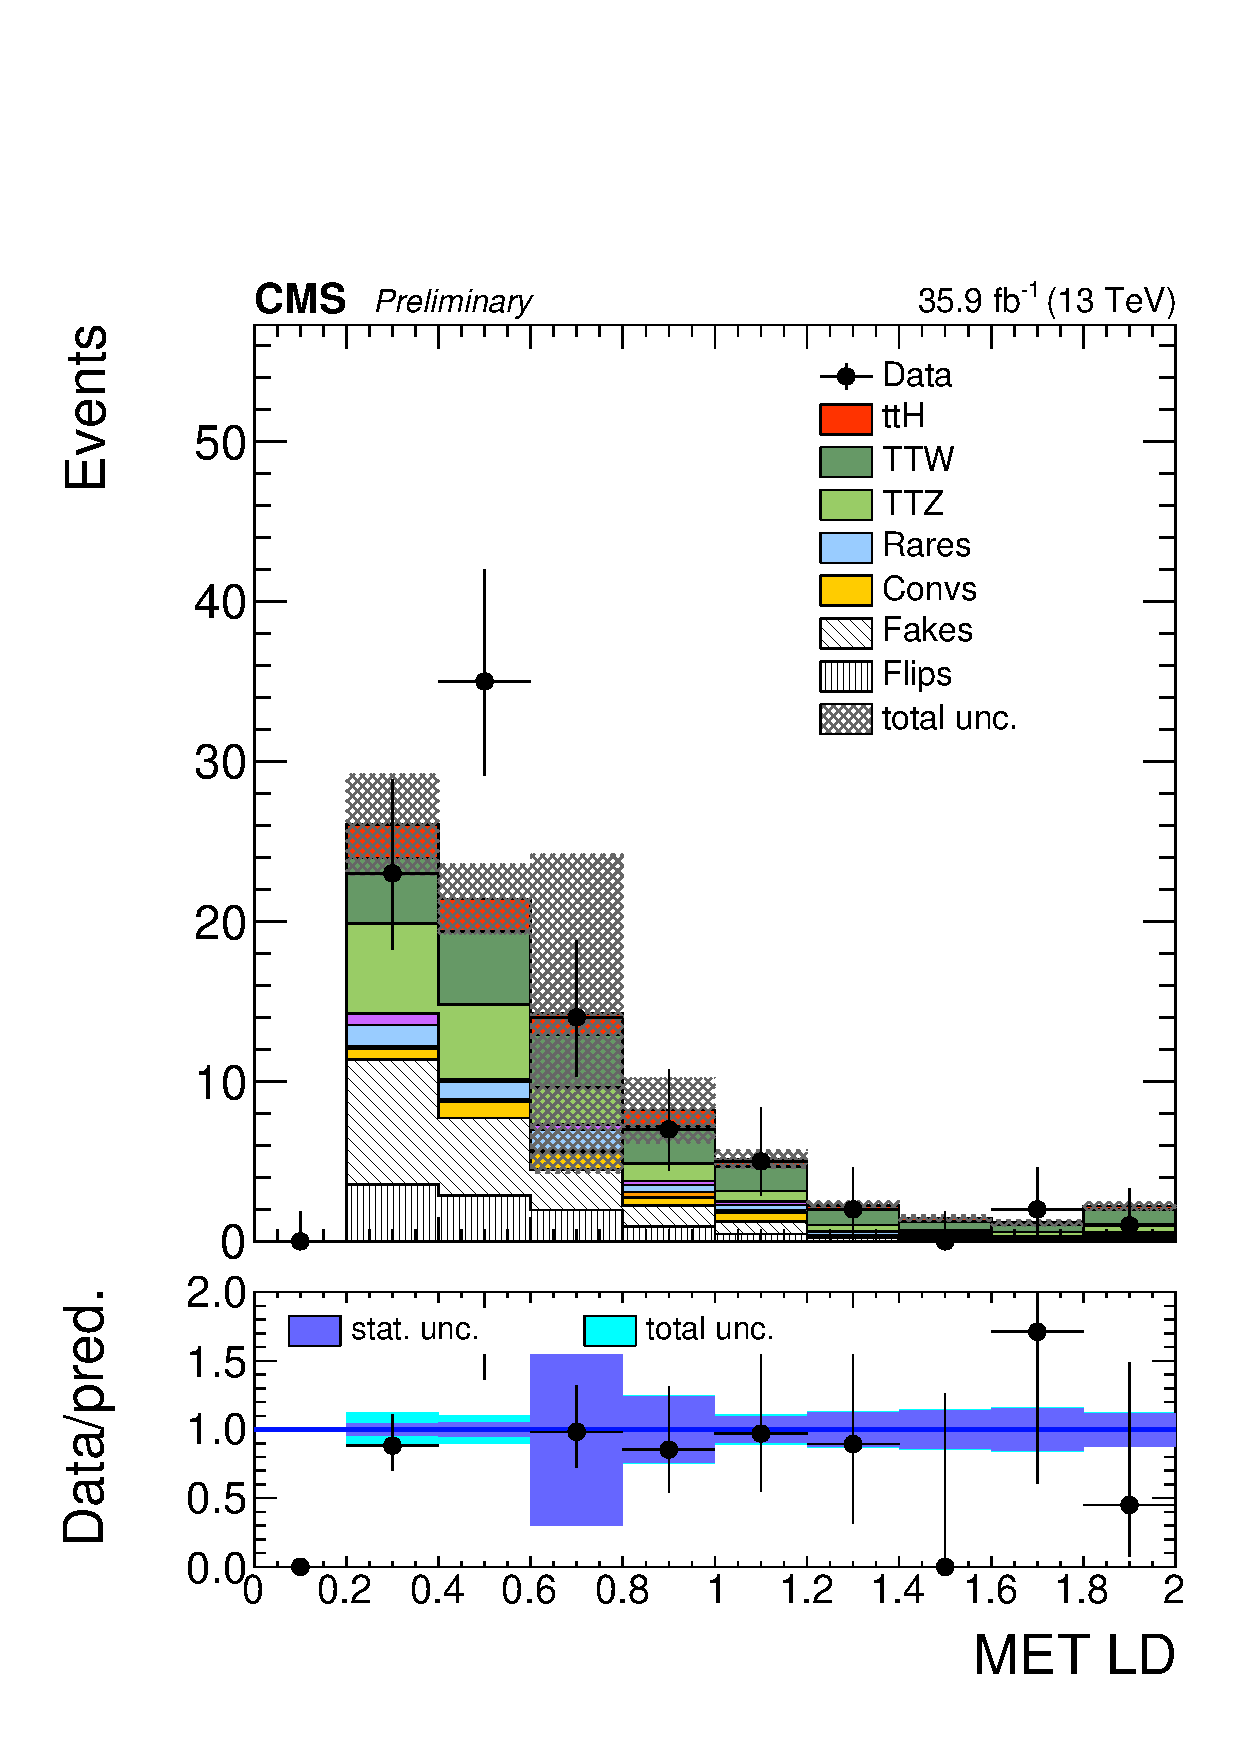
\includegraphics[width=0.32\textwidth]{plots_leptons/lep_evtsel/2lss_SR/ee/metLD.pdf}
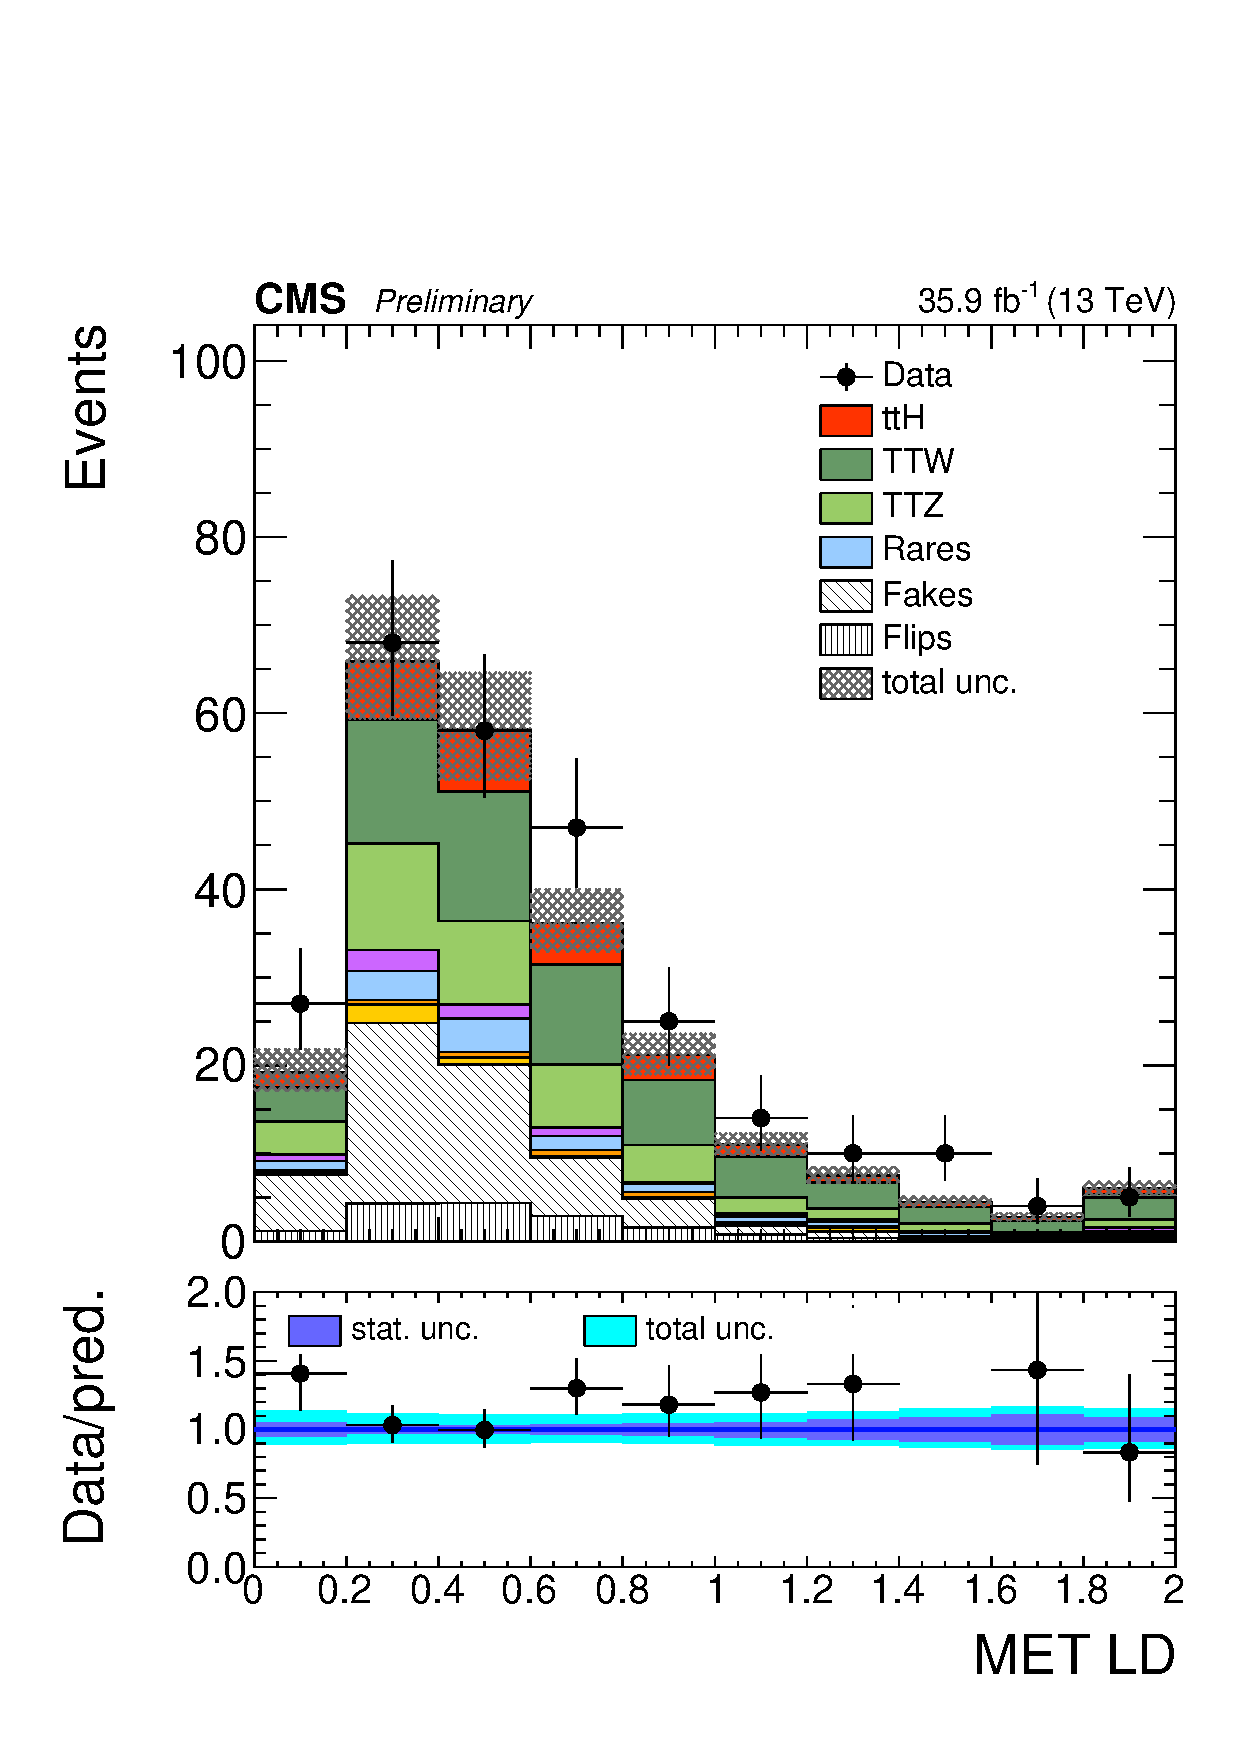
\includegraphics[width=0.32\textwidth]{plots_leptons/lep_evtsel/2lss_SR/em/metLD.pdf}
	\caption{$E_\mathrm{T}^\mathrm{miss}LD$ spectra in the 2$\ell$ ($\Pgm\Pgm$, $\Pe\Pe$, $\Pe\Pgm$) selections.}
	\label{fig:2l_metLD}
\end{figure}


%%%%%
%%   3l plots
%%%%%

%\begin{figure}[htb]
%	\centering 
%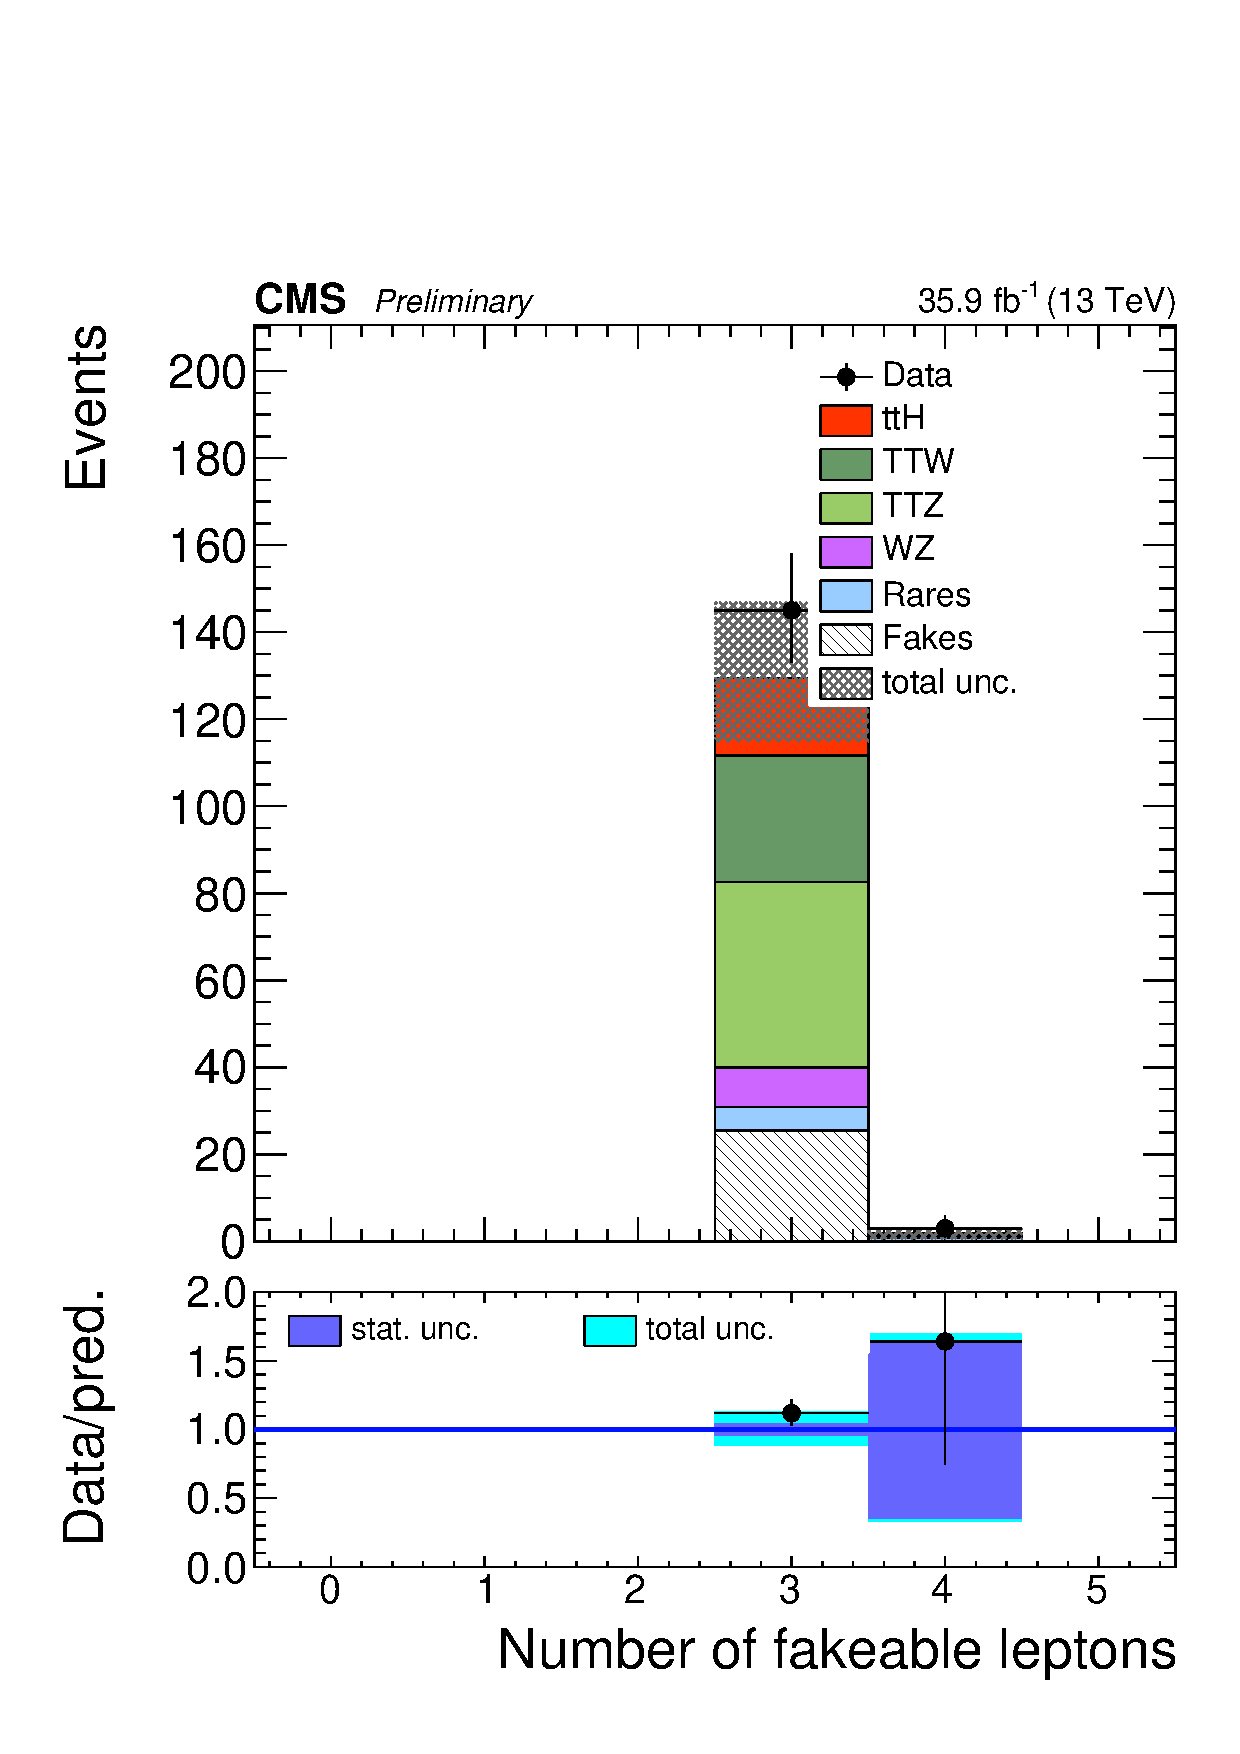
\includegraphics[width=0.32\textwidth]{plots_leptons/lep_evtsel/3l_SR/nLepFO.pdf}
%%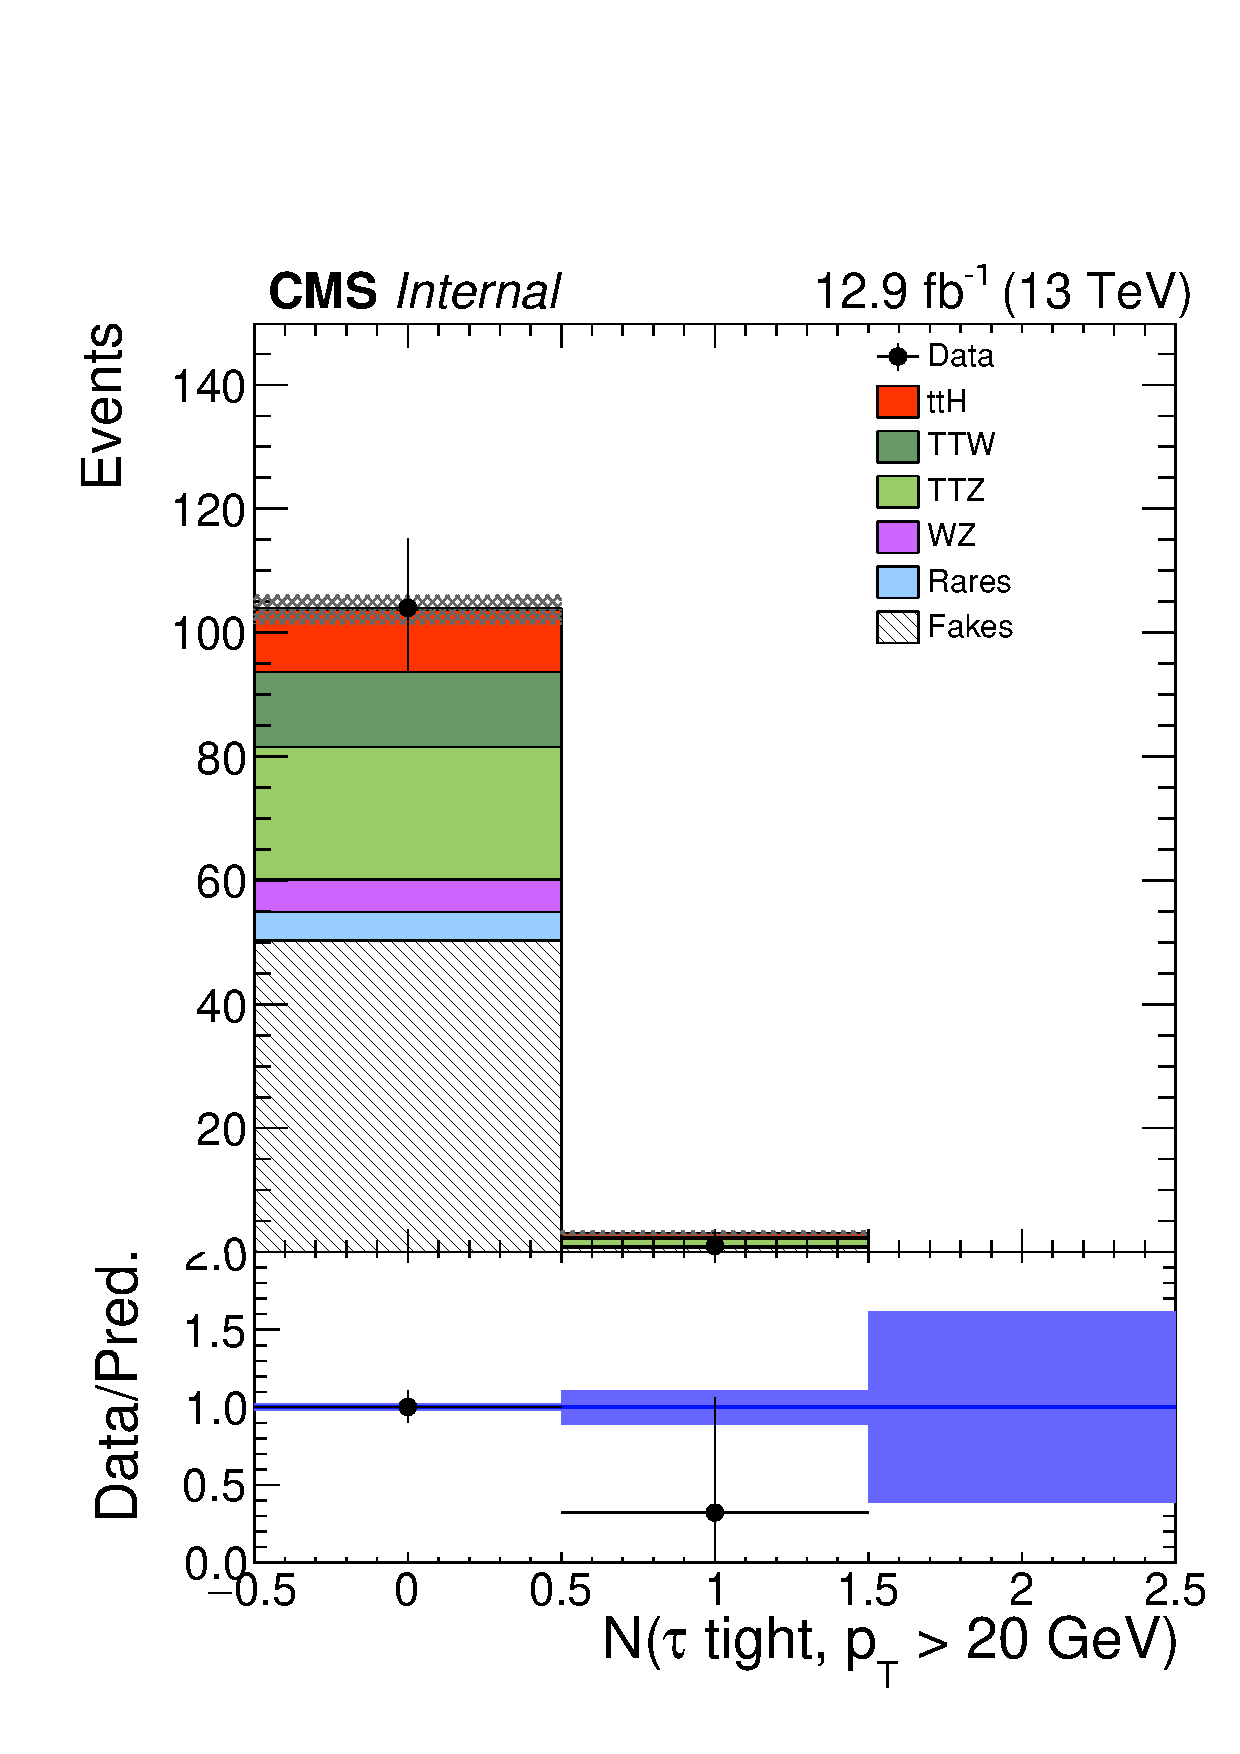
\includegraphics[width=0.32\textwidth]{plots_leptons/lep_evtsel/3l_SR/nTauTight.pdf}
%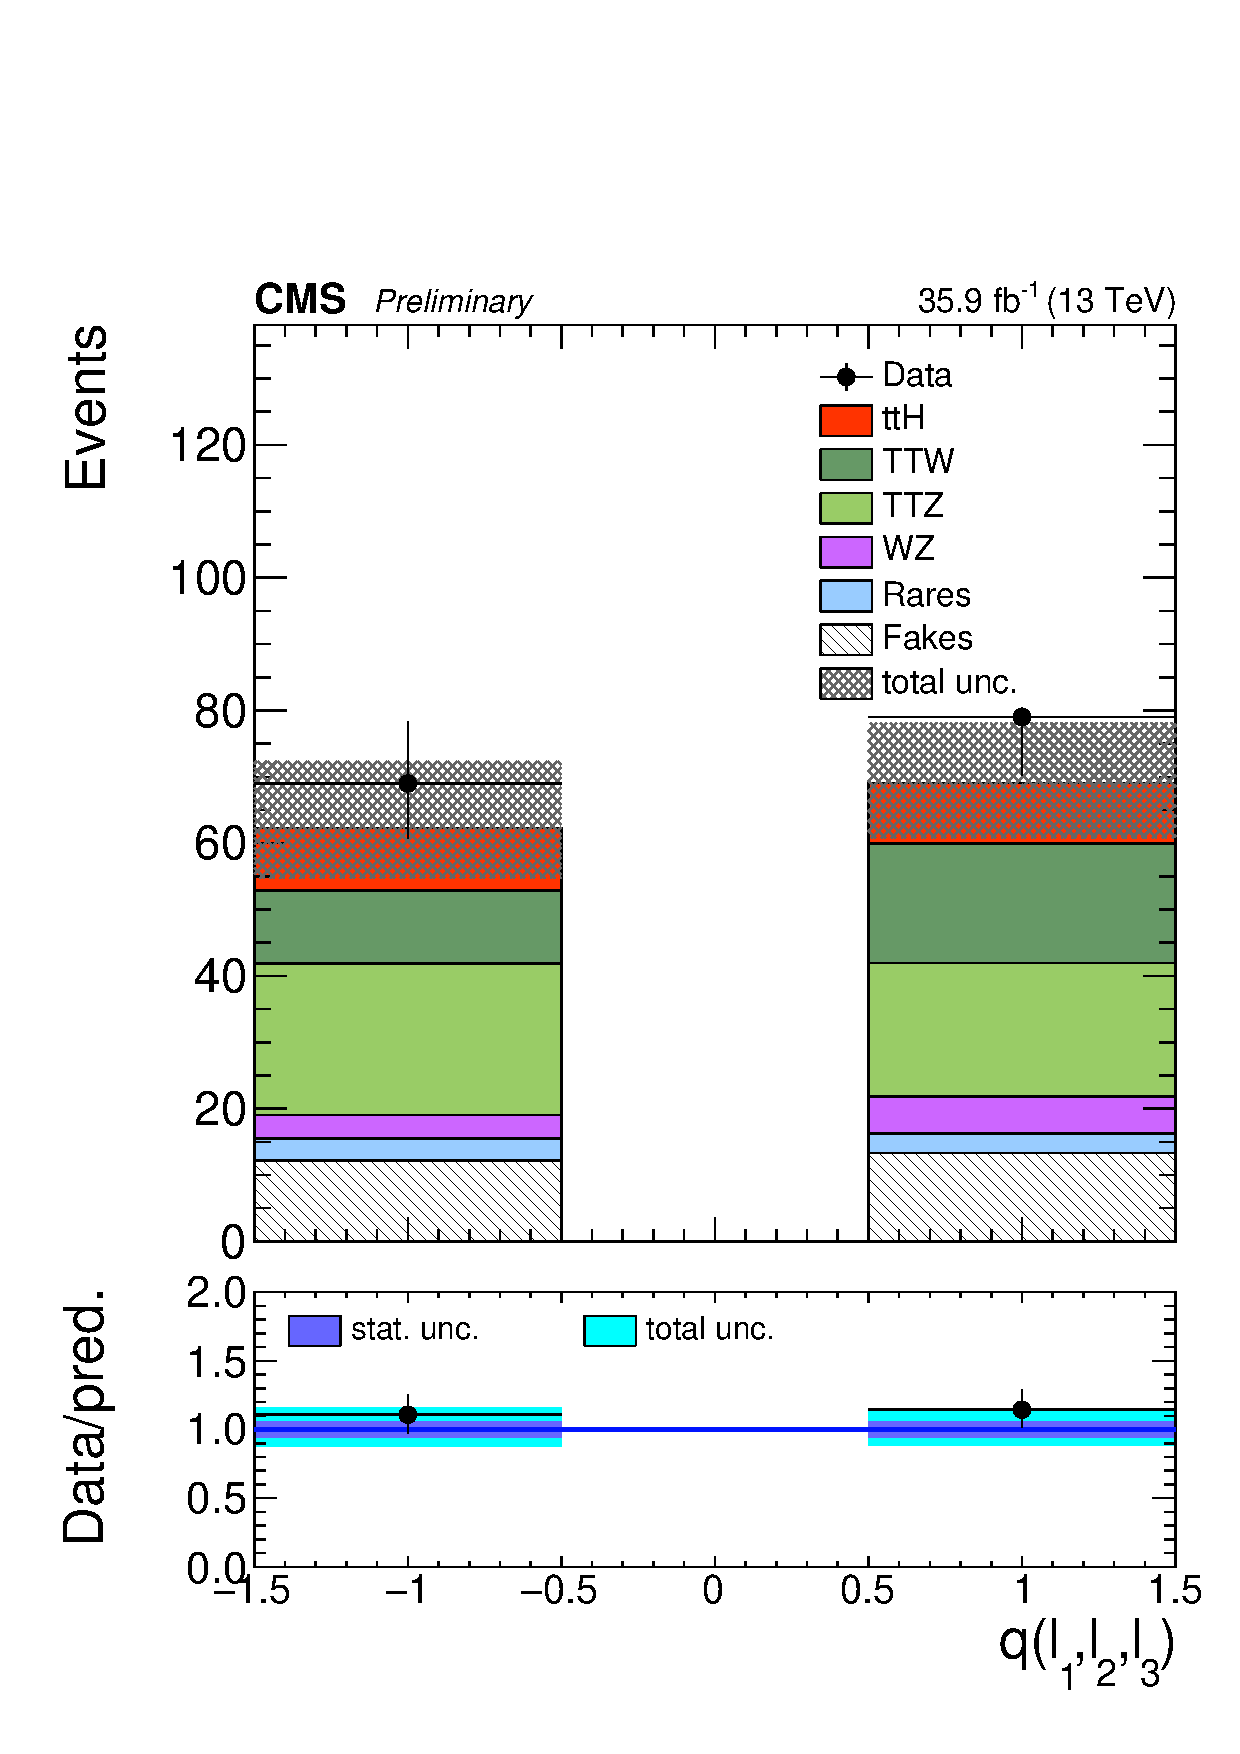
\includegraphics[width=0.32\textwidth]{plots_leptons/lep_evtsel/3l_SR/3lep_charge.pdf}
%	\caption{Number and charge of leptons passing the fakeable object requirements and $\Pgth$ leptons passing the requirements described in Section~\ref{subsec:taus} in the 3$\ell$ selection.}
%	\label{fig:3l_nLepFO}
%\end{figure}

\begin{figure}[htb]
	\centering 
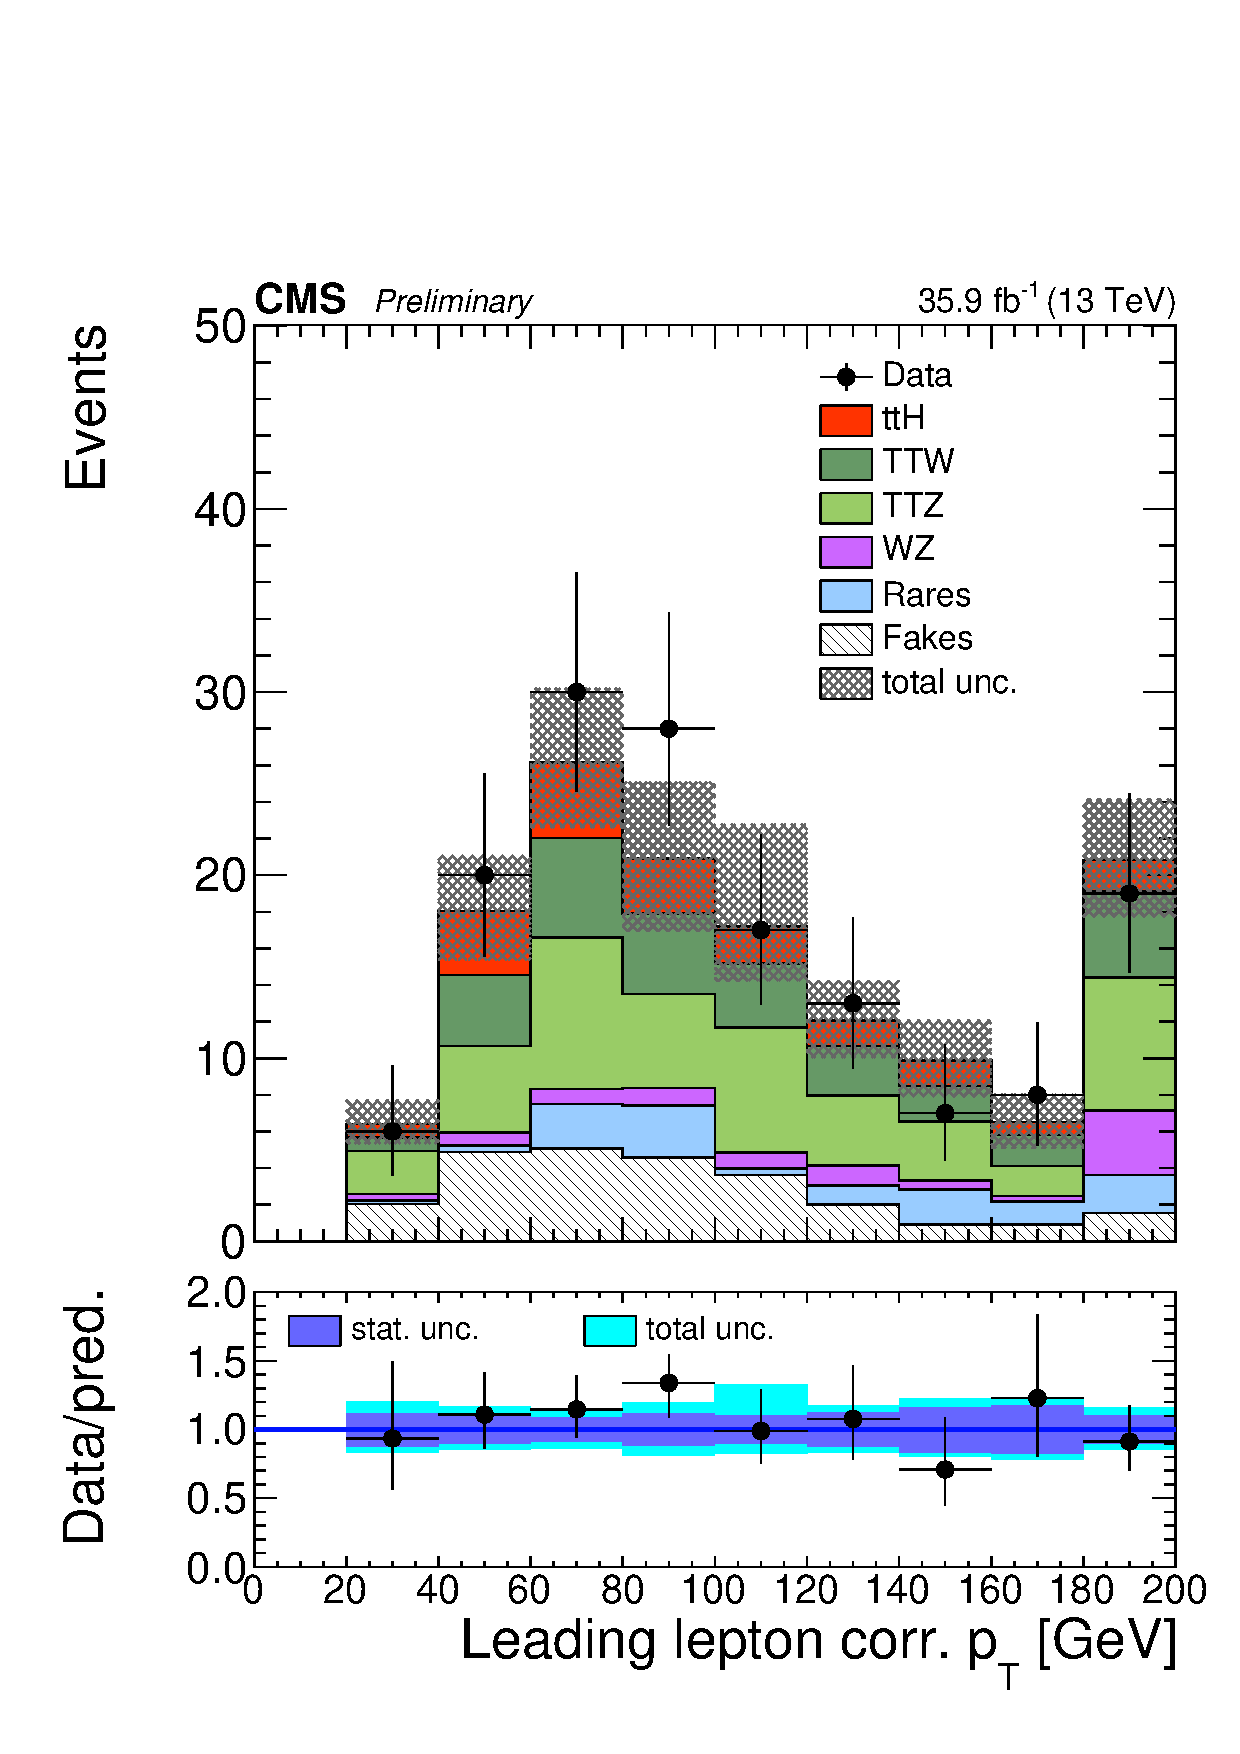
\includegraphics[width=0.32\textwidth]{plots_leptons/lep_evtsel/3l_SR/kinMVA_input_LepGood0_conePt.pdf}
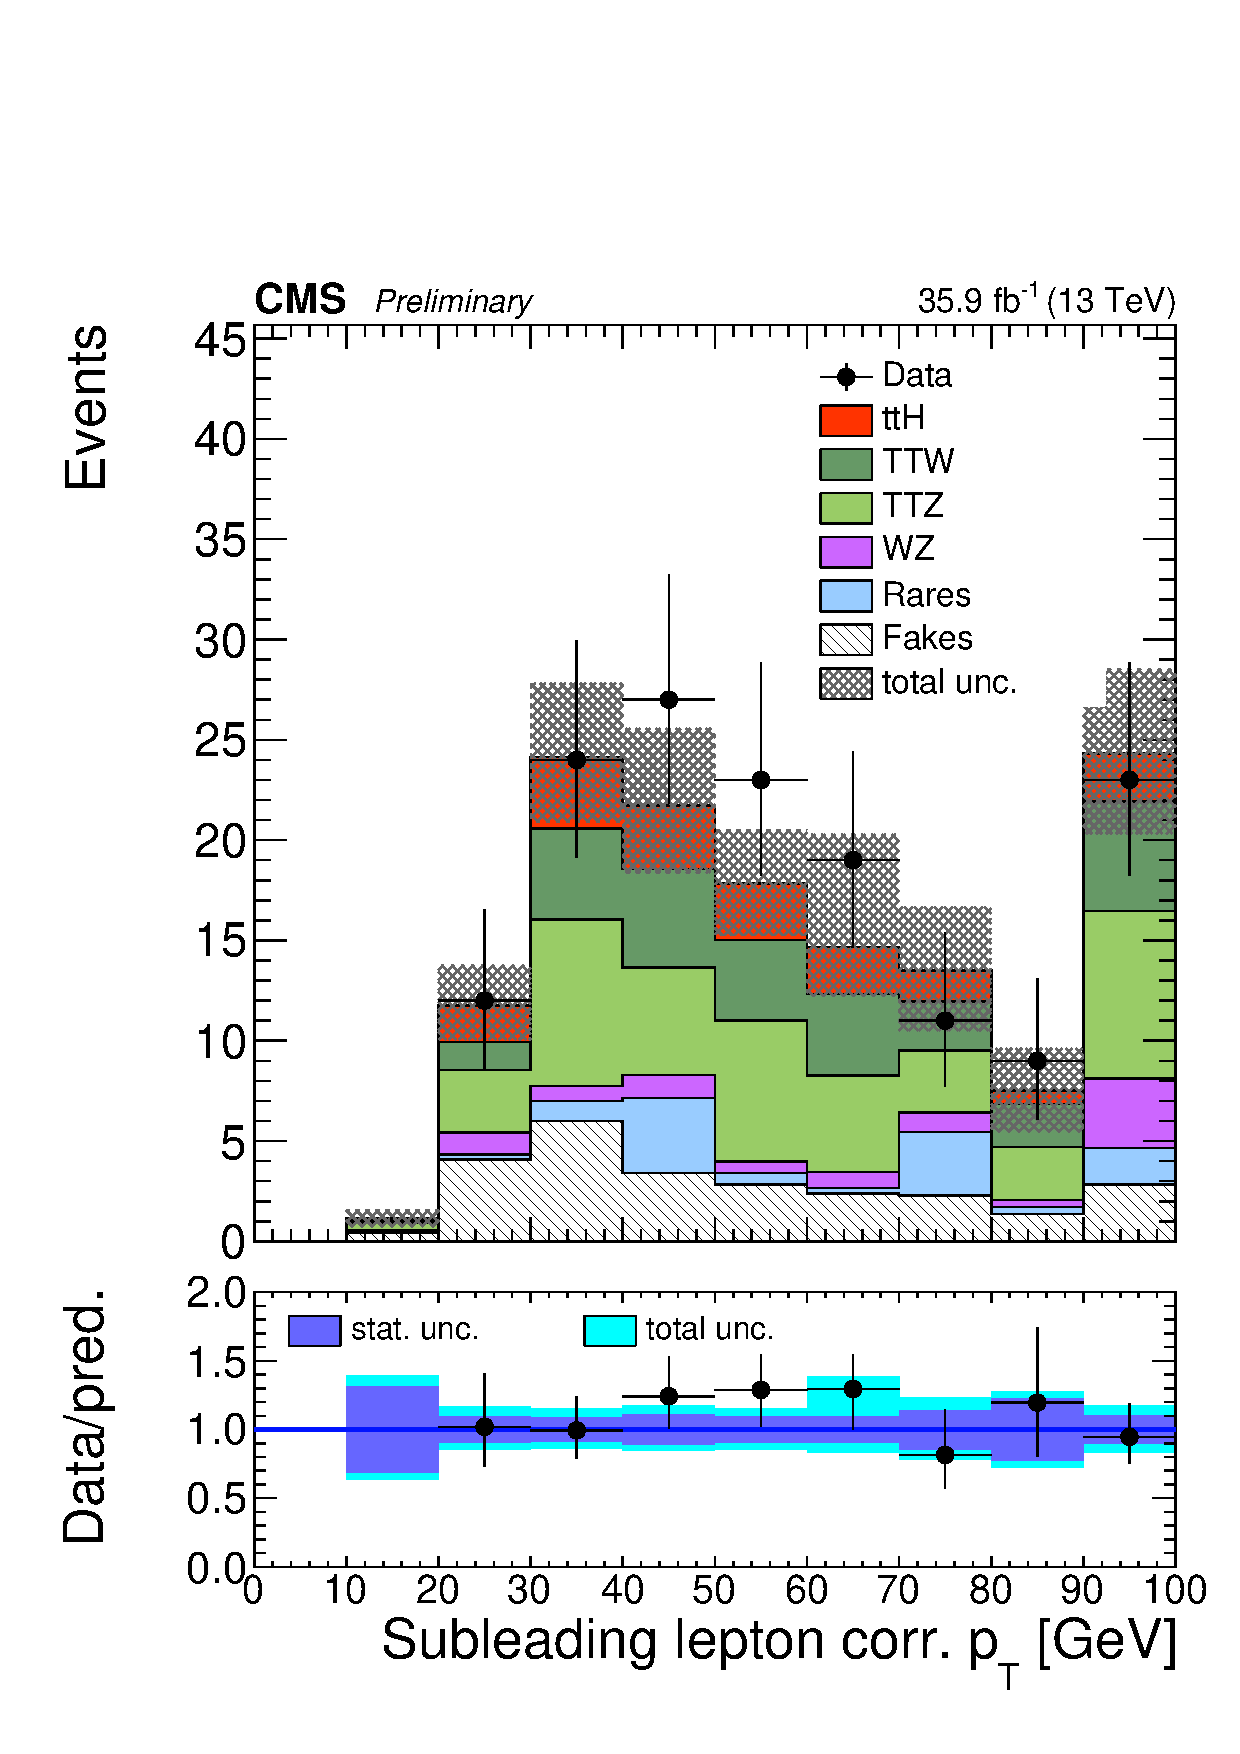
\includegraphics[width=0.32\textwidth]{plots_leptons/lep_evtsel/3l_SR/kinMVA_input_LepGood1_conePt.pdf}
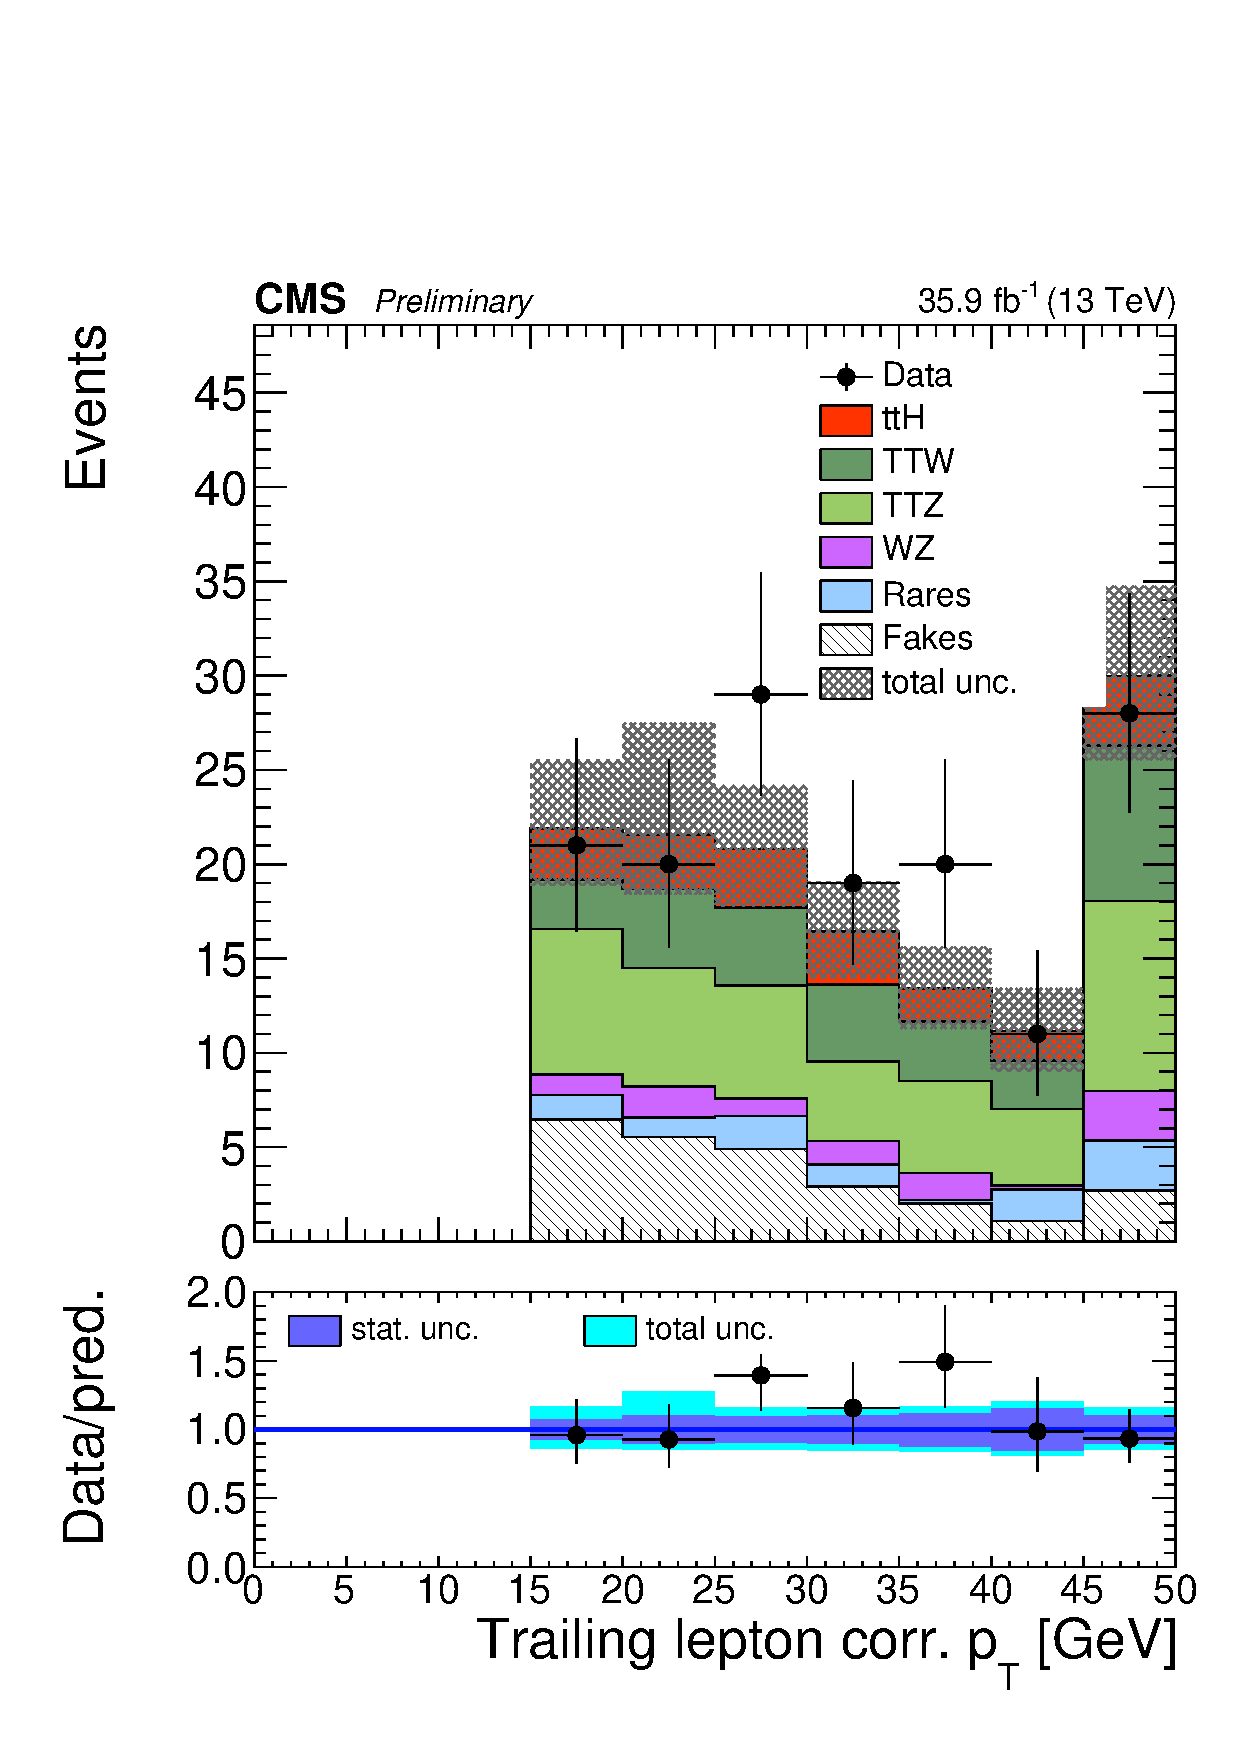
\includegraphics[width=0.32\textwidth]{plots_leptons/lep_evtsel/3l_SR/kinMVA_input_LepGood2_conePt.pdf}
	\caption{Lepton transverse momentum spectra in the 3$\ell$ selection.}
	\label{fig:3l_lepPt}
\end{figure}

\begin{figure}[htb]
	\centering 
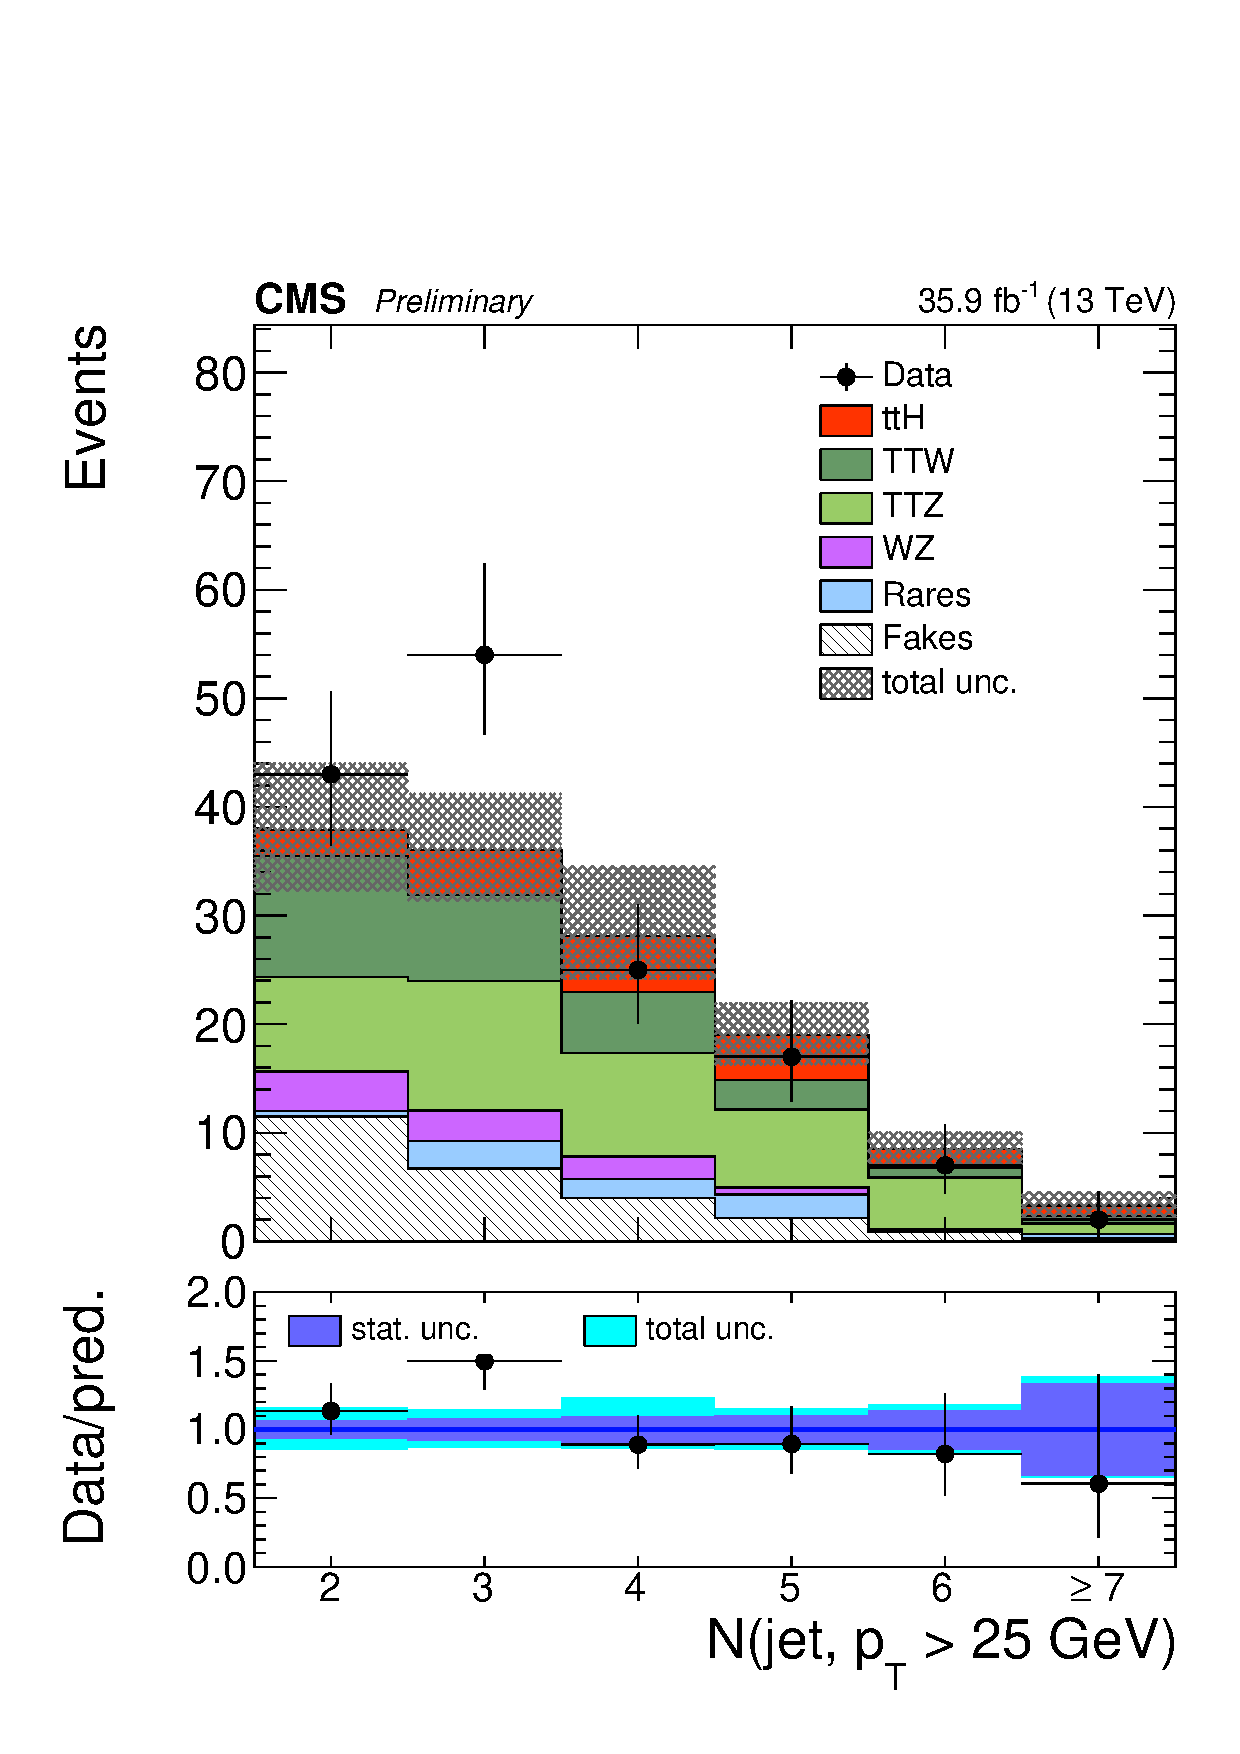
\includegraphics[width=0.32\textwidth]{plots_leptons/lep_evtsel/3l_SR/3lep_nJet25.pdf}
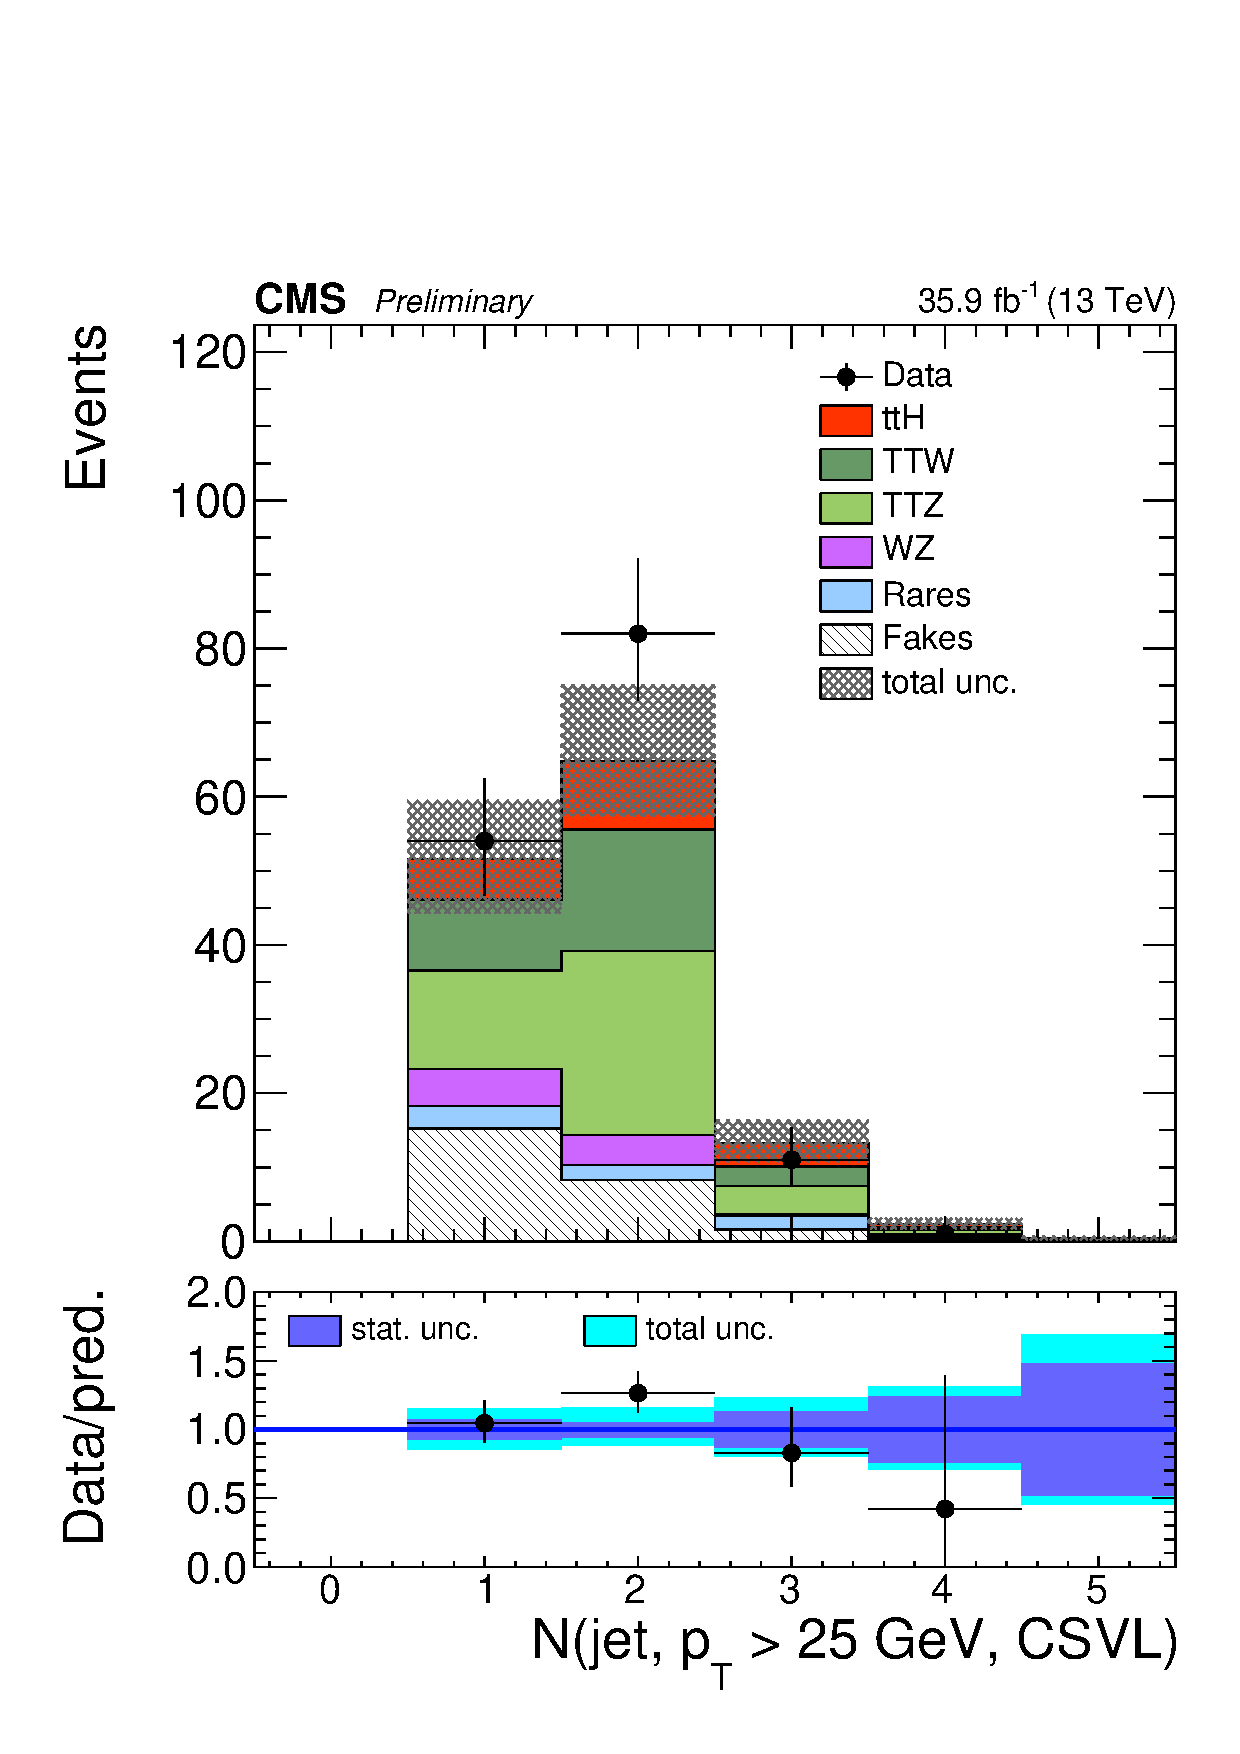
\includegraphics[width=0.32\textwidth]{plots_leptons/lep_evtsel/3l_SR/nBJetLoose25.pdf}
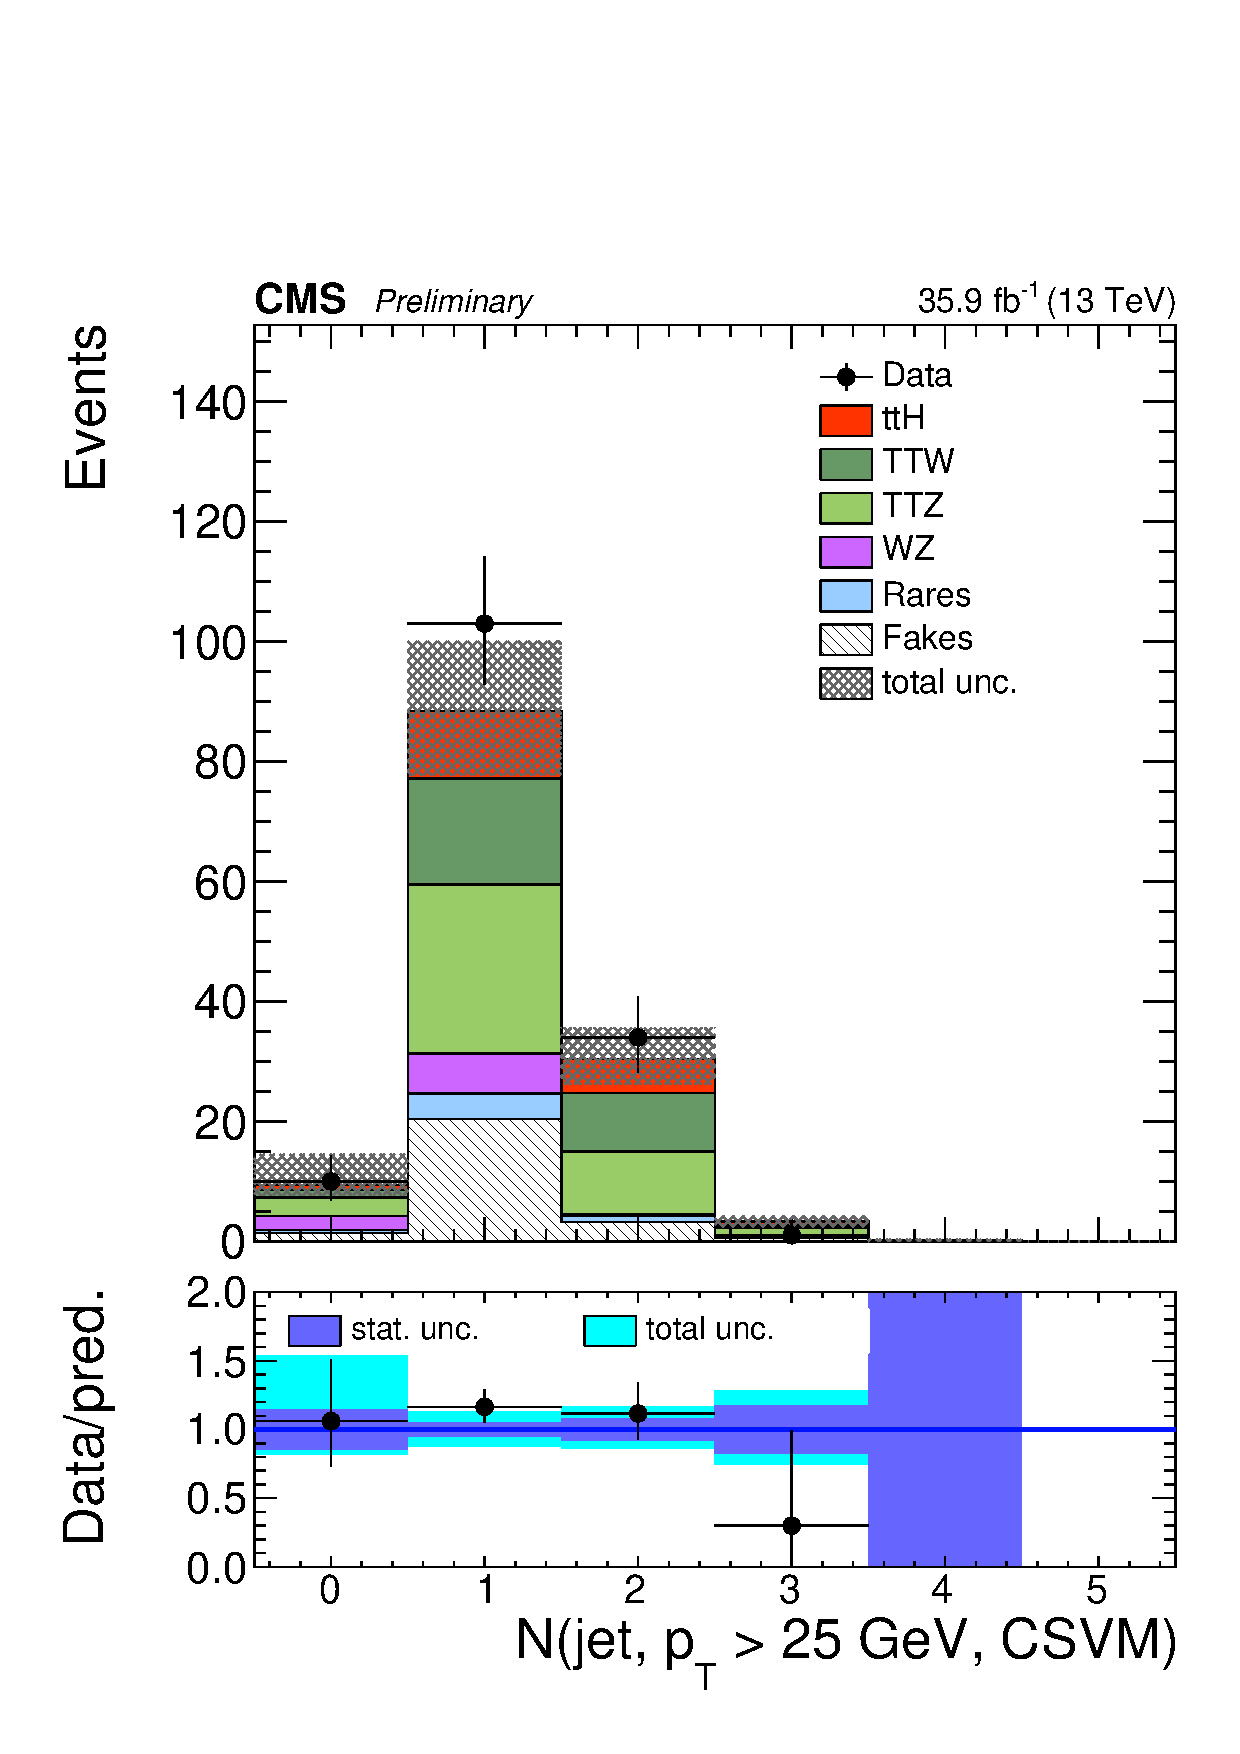
\includegraphics[width=0.32\textwidth]{plots_leptons/lep_evtsel/3l_SR/nBJetMedium25.pdf}
	\caption{Jet multiplicities (all jets, jets passing the loose working point of the CSV tagger, jets passing the medium working point of the CSV tagger) in the the 3$\ell$ selection.}
	\label{fig:3l_nJet}
\end{figure}

\begin{figure}[htb]
	\centering 
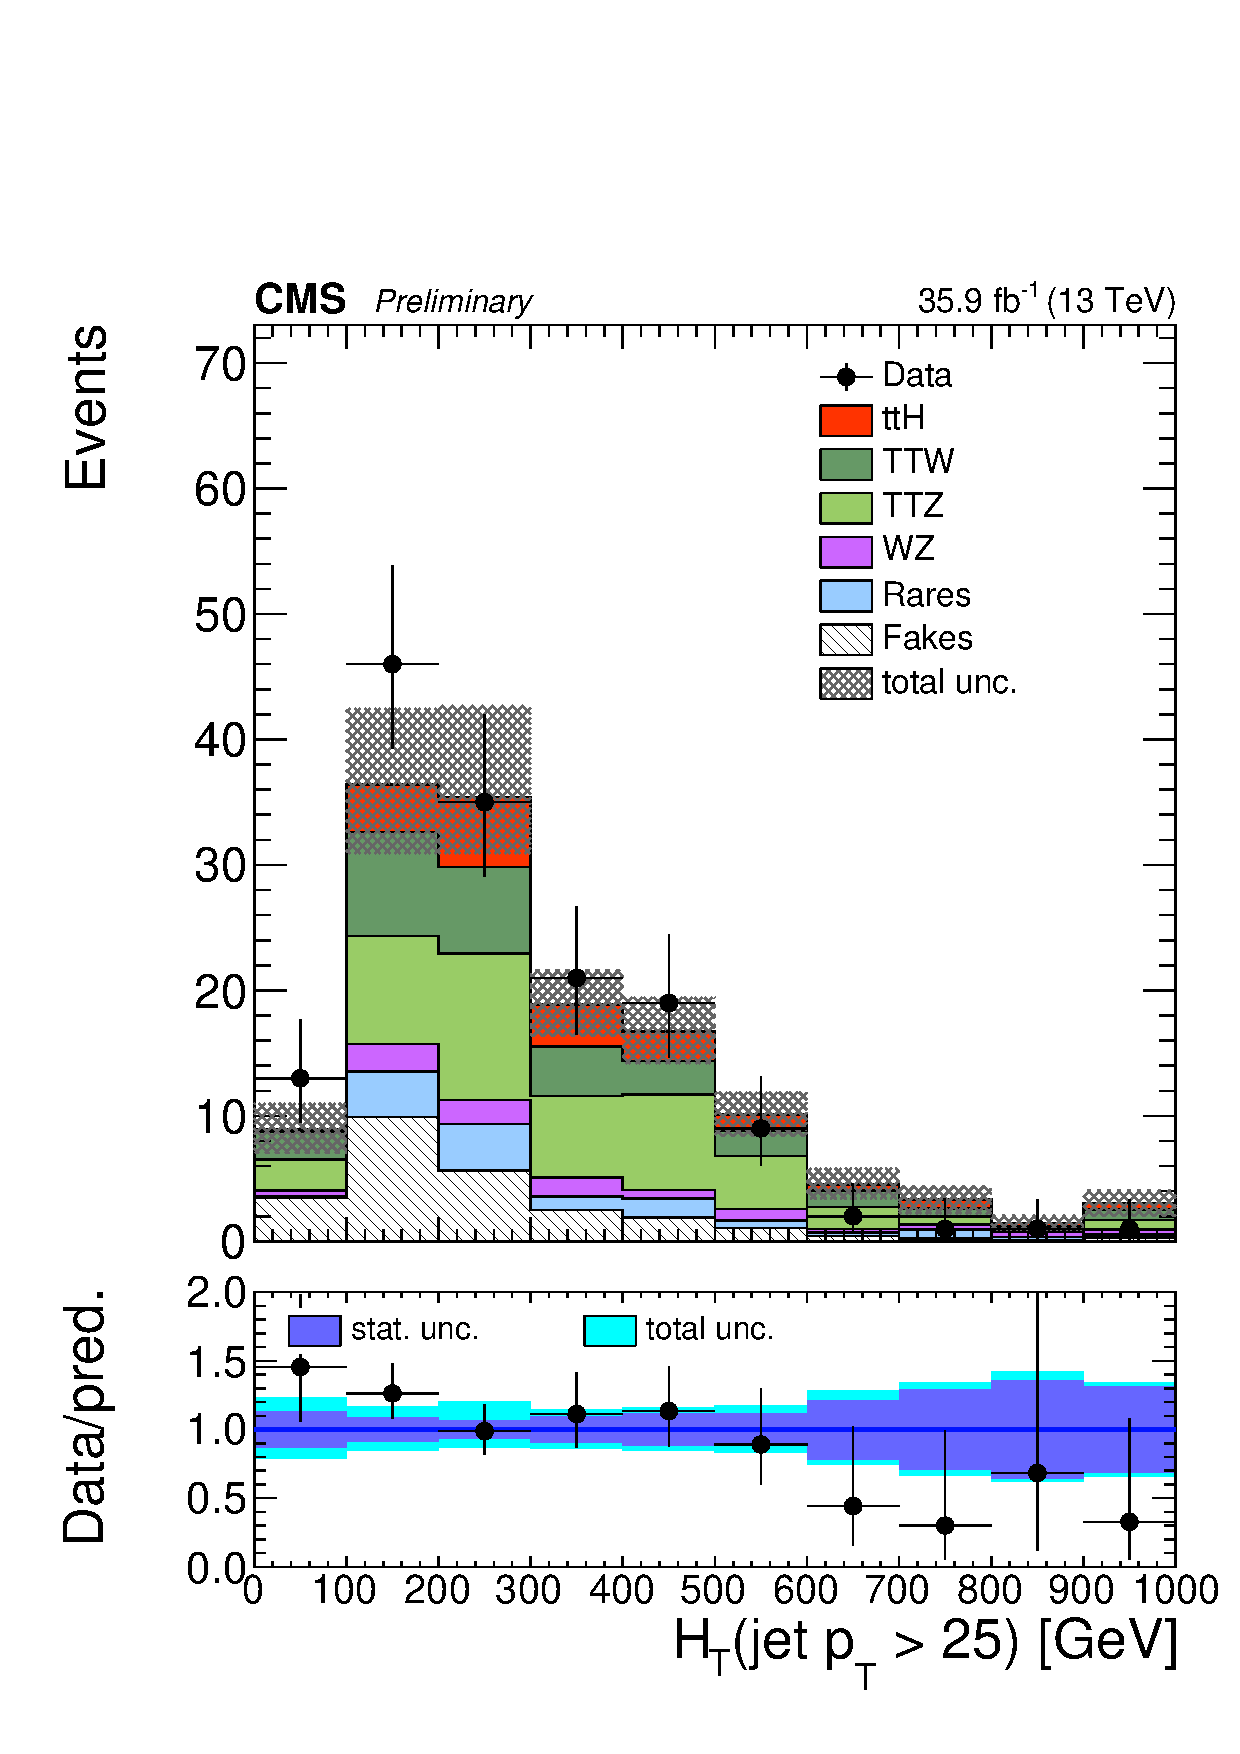
\includegraphics[width=0.32\textwidth]{plots_leptons/lep_evtsel/3l_SR/htJet25j.pdf}
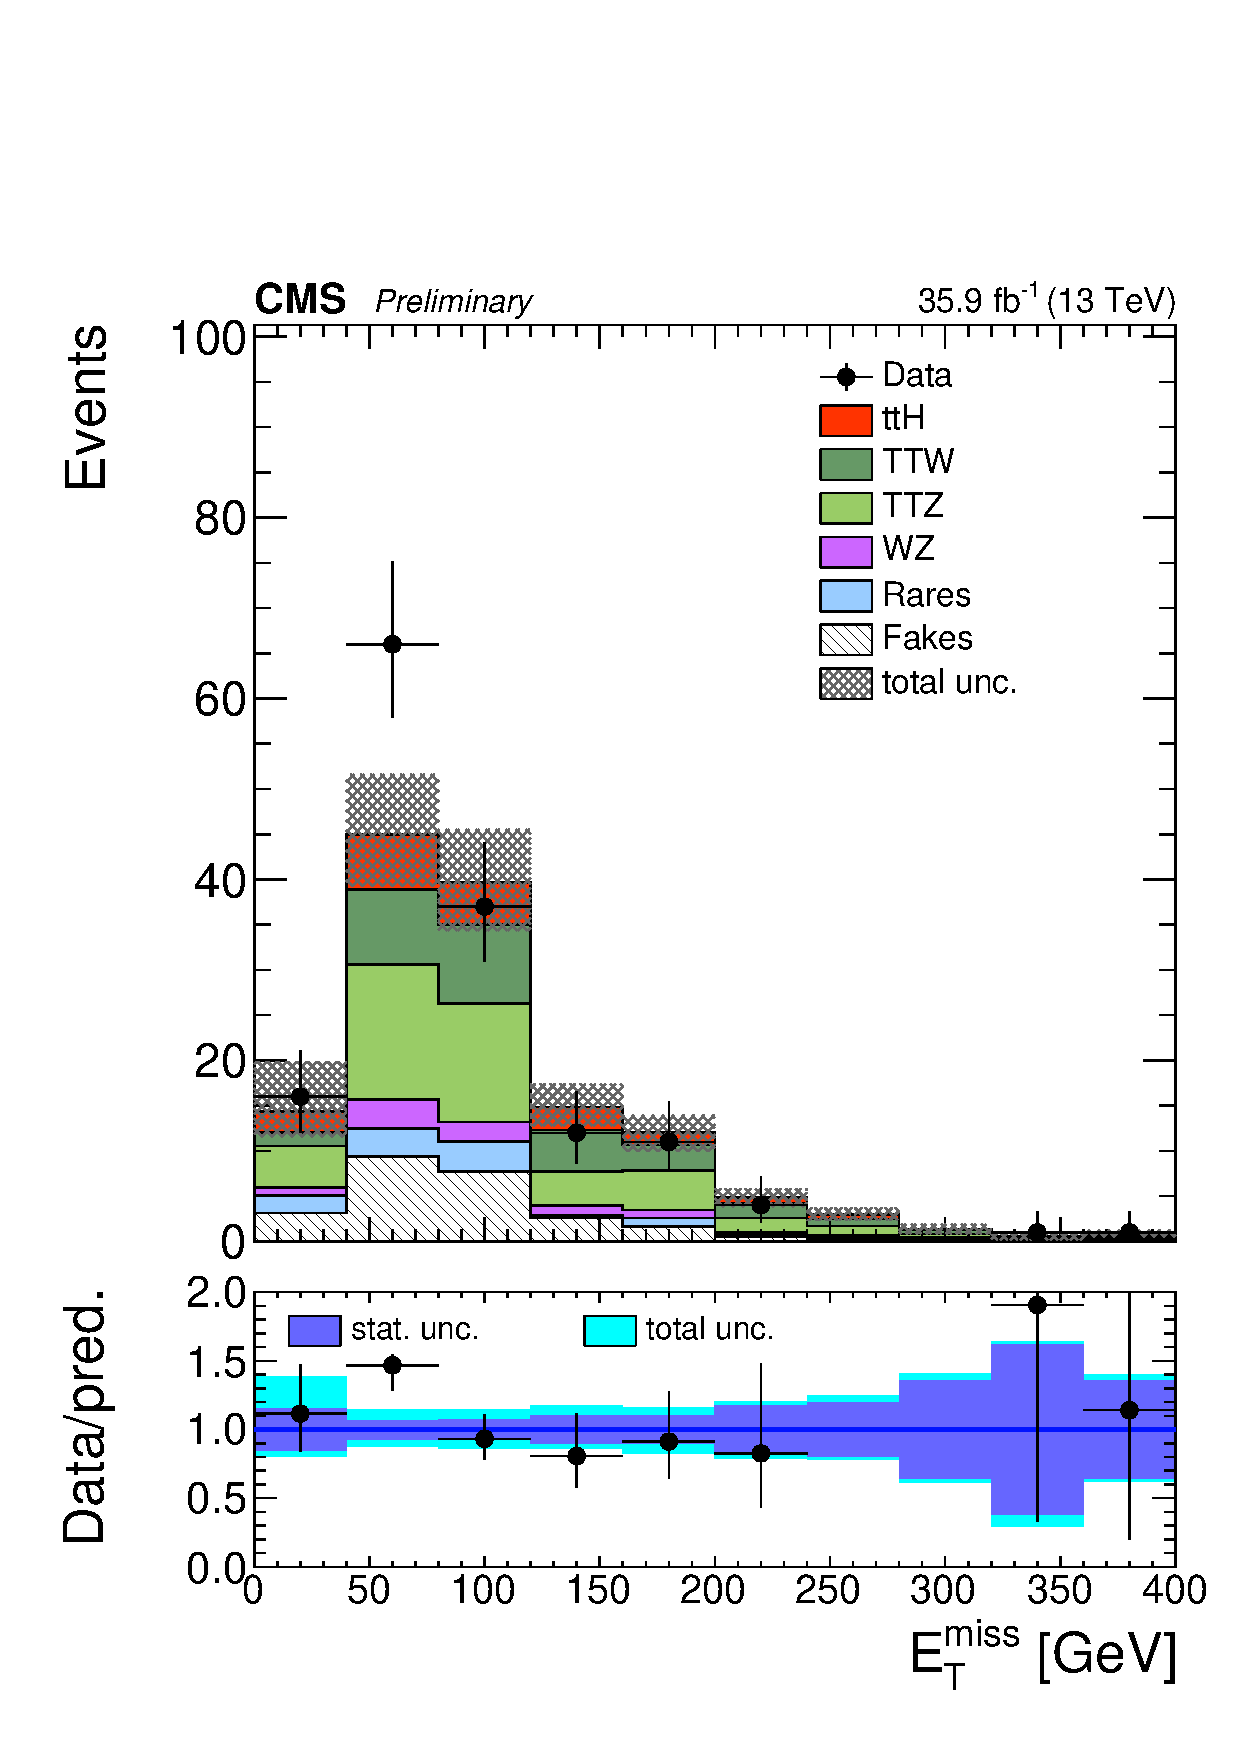
\includegraphics[width=0.32\textwidth]{plots_leptons/lep_evtsel/3l_SR/met.pdf}
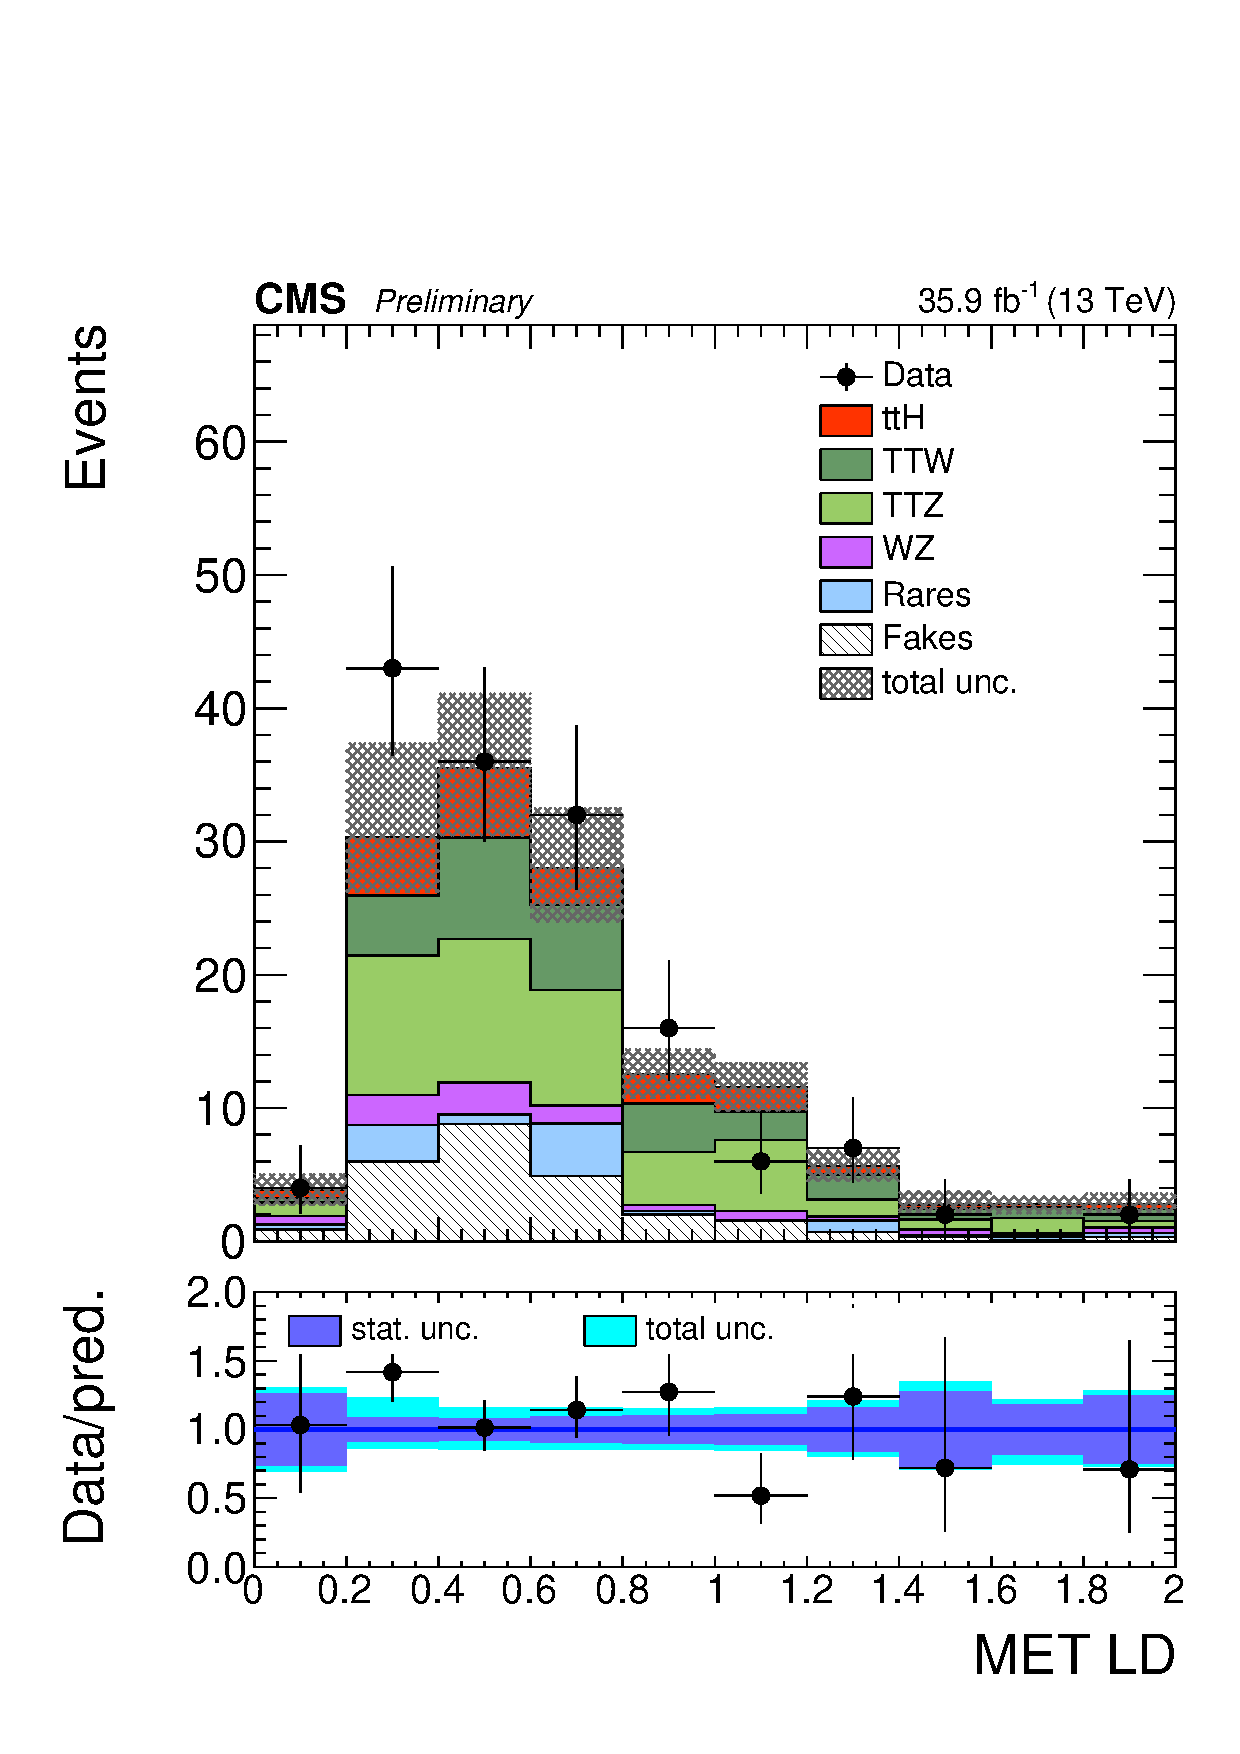
\includegraphics[width=0.32\textwidth]{plots_leptons/lep_evtsel/3l_SR/metLD.pdf}
	\caption{$H_T$, $E_\mathrm{T}^\mathrm{miss}$ and $E_\mathrm{T}^\mathrm{miss}LD$ distributions in the 3$\ell$ selection.}
	\label{fig:3l_ht}
\end{figure}

%%%%%
%%   4l plots
%%%%%
\begin{figure}[htb]
	\centering 
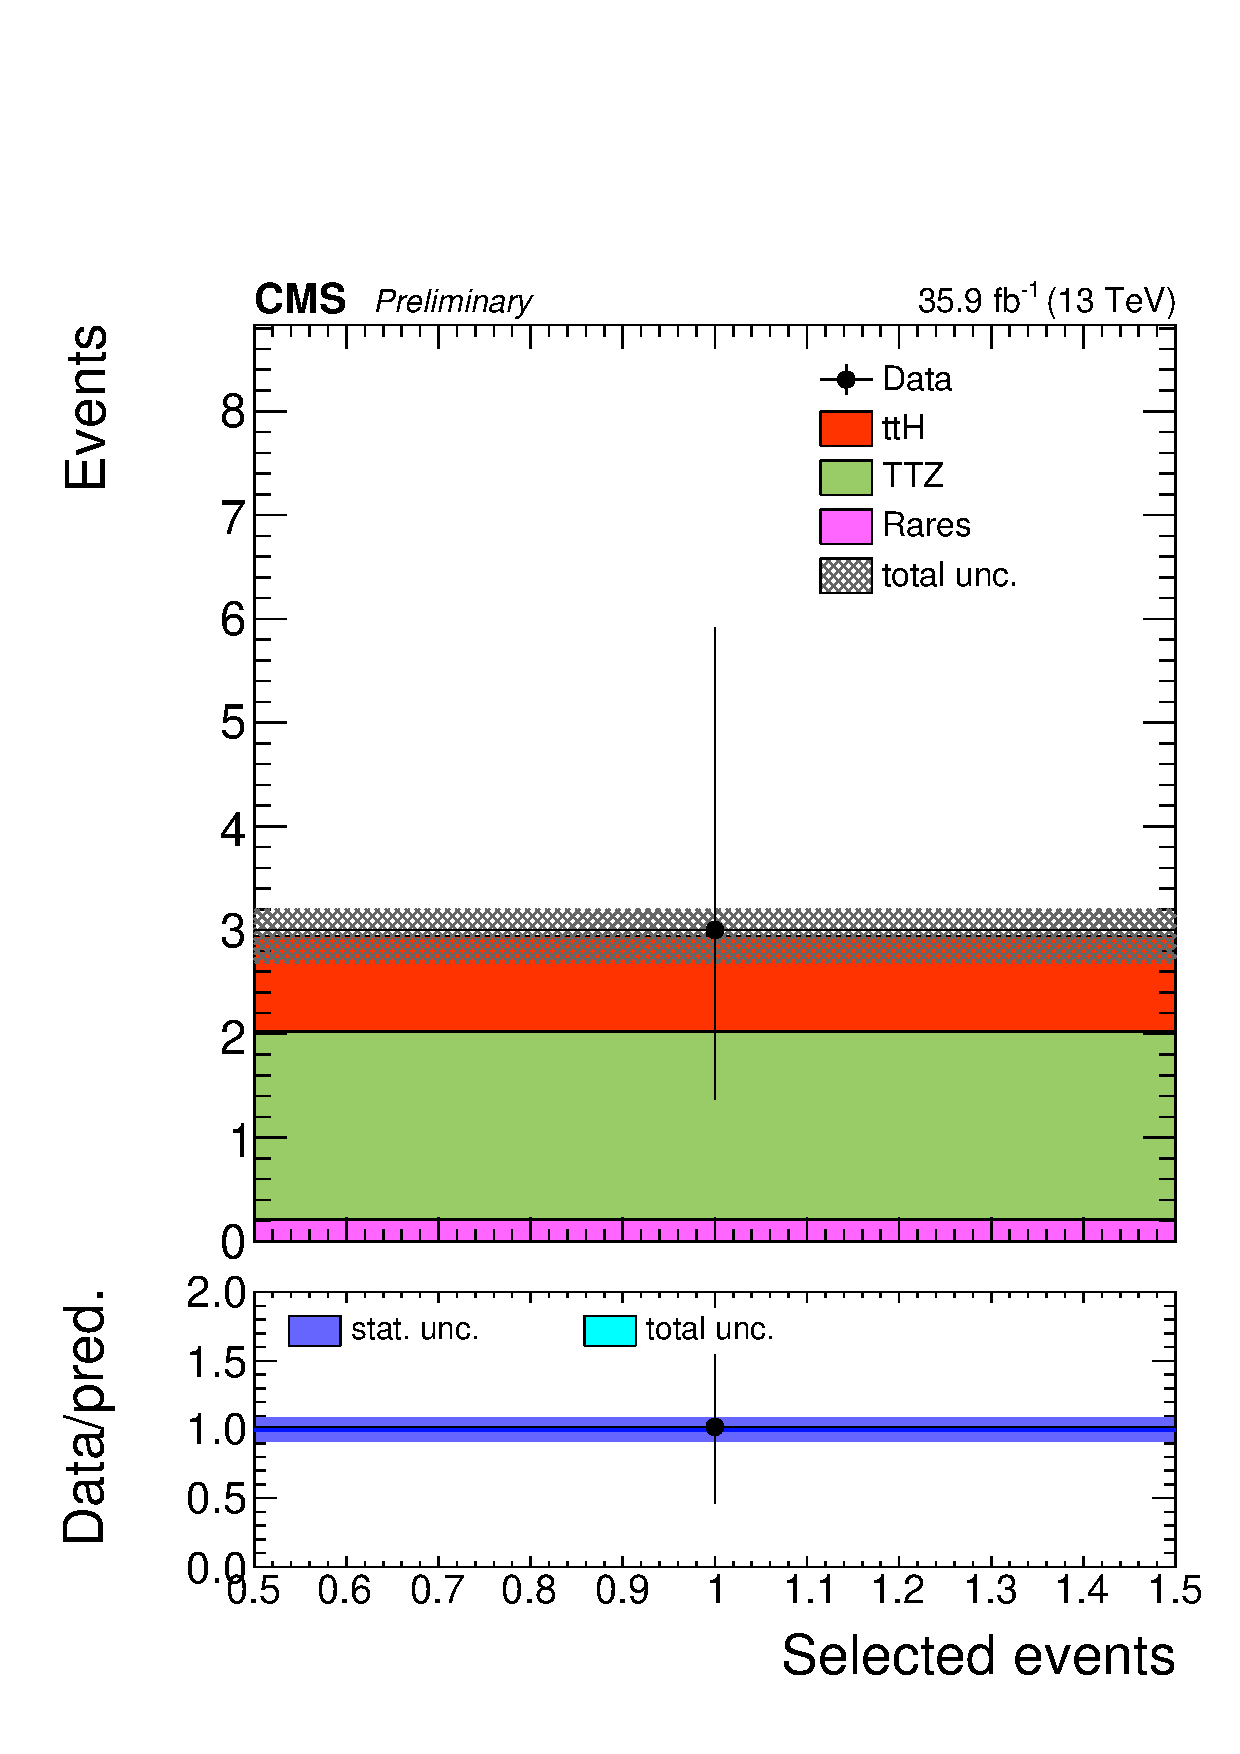
\includegraphics[width=0.32\textwidth]{plots_leptons/lep_evtsel/4l_SR/tot_weight.pdf}
	\caption{Number of events selected in the $4\ell$ category.}
	\label{fig:4l_numevt}
\end{figure}

%% flush plots
\clearpage
